\documentclass[AMA,final,STIX1COL]{WileyNJD-v2}

\usepackage{xspace}
\usepackage{comment}
\usepackage{subfigure}
\articletype{Research Article}
\received{20 April, 2020}
\revised{TBD}
\accepted{TBD}

\raggedbottom

\def\COMPANION{{\scriptsize\url{https://gitlab.com/msserpa/prefetcher-ccpe}}\xspace}

\newcommand\new[1]{{\color{red}\textbf{#1}}}
\newcommand{\ms}[1]{\textcolor{orange}{\bfseries \ul{ msserpa: #1} }\vspace{0.2cm}}
\newcommand{\vsg}[1]{\textcolor{blue}{\bfseries \ul{vsgirelli: #1} }\vspace{0.2cm}}
\newcommand{\fbm}[1]{\textcolor{red}{\bfseries \ul{fbm: #1} }\vspace{0.2cm}}

\begin{document}

\title{Investigating Memory Prefetcher Performance over Parallel Applications: From Real to Simulated}

\author{Valéria S. Girelli*}
\author{Francis B. Moreira}
\author{Matheus S. Serpa}
\author{Danilo Carastan-Santos}
\author{Philippe O. A. Navaux}

\address{
  \orgdiv{Informatics Institute},%navaux prefere sem o of...
  \orgname{Federal University of Rio Grande do Sul -- UFRGS},
  \orgaddress{\city{Porto Alegre}, \country{Brazil}}}

\corres{*Valéria S. Girelli, UFRGS, Bento Gon\c{c}alves 9500, Porto Alegre -- RS, Brazil. \email{vsgirelli@inf.ufrgs.br}}

\authormark{Girelli \textsc{et al}}


\abstract[Summary]{
%%%% 177 WORD ABSTRACT%%%%%%%%%%%%%%%%%%%%%%%%%%%%%%%%%%%%%%%%%%%%%%%%%%%%%%%%%%%%%%%%%%%%%%%%%%%%%%%
Memory prefetcher algorithms are widely used in processors to mitigate the performance gap between the processors and the memory subsystem. 
The complexities behind the architectures and prefetcher algorithms, however, not only hinder the development of accurate architecture simulators, but also hinder understanding the prefetcher's contribution to performance, on both a real hardware and in a simulated environment.
%Analyzing and developing new prefetcher algorithms is possible thanks to architecture simulators that model the highly complex interactions present in the hardware. When we account for parallel, High-Performance Computing (HPC) applications, understanding the prefetcher's contribution to performance, on both the real hardware and in the simulations, becomes challenging. 
In this paper, we contribute to shed light the memory prefetcher's role in the performance of parallel HPC applications, considering the prefetcher algorithms offered by both the real hardware and the simulators. 
\new{We performed a careful experimental investigation}, executing the NAS parallel benchmark (NPB) on a real Skylake machine, and as well in a simulated environment with the ZSim and Sniper simulators, taking into account the prefetcher algorithms offered by both Skylake and the simulators. 
%In this paper, we provide a better understanding of the memory prefetcher's role in the performance of HPC applications, considering the prefetcher algorithms offered by both the real hardware and the simulators. We performed a careful experimental campaign, executing the NAS parallel benchmark (NPB) on a real Skylake machine, and as well in a simulated environment with the ZSim and Sniper simulators, taking into account the prefetcher algorithms offered by both Skylake and the simulators. 
Our experimental results show that: (i) prefetching from the L3 to L2 cache presents better performance gains, (ii) the memory contention in the parallel execution constrains the prefetcher's effect, (iii) Skylake's parallel memory contention is poorly simulated by ZSim and Sniper, and (iv) Skylake's non-inclusive L3 cache hinders the accurate simulation of NPB with the Sniper's prefetchers.%\ms{deixar claro as contribuicoes aqui, na intro e na conclusao dcs: feito}
%%%%%%%%%%%%%%%%%%%%%%%%%%%%%%%%%%%%%%%%%%%%%%%%%%%%%%%%%%%%%%%%%%%%%%%%%%%%%%%%%%%%%%%%%%%%%%%%%%%%%

%%%% 209 WORD ABSTRACT%%%%%%%%%%%%%%%%%%%%%%%%%%%%%%%%%%%%%%%%%%%%%%%%%%%%%%%%%%%%%%%%%%%%%%%%%%%%%%%

%Memory prefetcher algorithms have been widely used in processors to mitigate the performance gap between the processors and the memory subsystem. Analyzing and developing new prefetcher algorithms is mainly possible thanks to architecture simulators that model the highly complex interactions present in the hardware. When we account for parallel, High-Performance Computing (HPC) applications, understanding the prefetcher's contribution to performance, on both the real hardware and in the simulations, becomes challenging. 
%In this paper, we provide a better understanding of the memory prefetcher's role in the performance of HPC applications, considering the prefetcher algorithms present in the real hardware and the ones present in simulators. For this task, we performed a careful experimental campaign, executing the NAS parallel benchmark (NPB) on a real Skylake machine, and as well in a simulated environment with the ZSim and Sniper simulators, taking into account all prefetcher algorithms offered by both Skylake and the simulators. 
%The highlights of our experimental results are: (i) prefetching from the L3 to L2 cache presents better performance gains, (ii) the memory contention in the parallel execution constrains the prefetcher's effect, (iii) Skylake's parallel memory contention is poorly simulated by ZSim and Sniper, and (iv) Skylake's non-inclusive L3 cache hinders the accurate simulation of NPB with the Sniper's prefetchers.

%%%%%%%%%%%%%%%%%%%%%%%%%%%%%%%%%%%%%%%%%%%%%%%%%%%%%%%%%%%%%%%%%%%%%%%%%%%%%%%%%%%%%%%%%%%%%%%%%%%%%

%Memory prefetcher algorithms have been widely used in processors to mitigate the performance gap between the processors and the memory subsystem. Analyzing and developing new prefetcher algorithms is mainly feasible thanks to architecture simulators, that model the highly complex interactions present in the hardware. When we account parallel, High Performance Computing (HPC) applications, understanding the prefetcher's contribution to performance, on both the real hardware and in the simulations, becomes challenging. 
%In this paper we provide a better understanding about the memory prefetcher's role in the performance of HPC applications, accounting the prefetcher algorithms present in the real hardware and the ones present in simulators. For this task we performed a careful experimental campaign executing the Numerical Aerodynamic Simulation Parallel Benchmark (NPB) in a real Skylake machine, and as well in a simulated environment with the ZSim and Sniper simulators, taking into account all prefetcher algorithms offered by both Skylake and the simulators. 
%Our experimental results show that (i) prefetching from the L3 to L2 cache presents a more substantial contribution to performance, (ii) memory contention becomes a larger constraint in the performance as the level of parallelism increases, limiting the prefetcher's contribution, (iii) Skylake's memory contention behavior is poorly simulated by ZSim and Sniper, and (iv) the Skylake's non-inclusive L3 cache and the concealment behind its prefetcher algorithms hinders accuretely simulating HPC applications with Sniper and its prefetchers.
}

\keywords{
computer architecture, 
parallel architecture, 
prefetcher, 
architecture simulation
}

\jnlcitation{\cname{
\author{V. S. Girelli},
\author{F. B. Moreira},
\author{M. S. Serpa},
\author{D. Carastan-Santos}, and
\author{P. O. A. Navaux}} (\cyear{2020}),
%\ctitle{Understanding Memory Prefetcher Performance over Parallel Applications: From Real to Simulated},
\ctitle{Investigating Memory Prefetcher Performance over Parallel Applications: From Real to Simulated},\cjournal{Concurrency and Computation: Practice and Experience}, \cvol{TBD}.}

\maketitle

\section{Introduction}\label{sec:introduction}

%=============== INTRODUCTION 100 GRAMMARLY SCORE!================================================
In recent years, there have been significant advances in the performance of processors, exemplified by the reduction of transistor size and the increase in the number of cores in a processor. %~\fbm{requires citation. processor freq increases in recent years? I'm doubtful}. 
%However, the amount of data required by the processors to operate efficiently steadily increased as well~\fbm{the less data the better, actually. this sentence doesn't make sense, rather, the demand for data to be processed has increased, and while the processor core design has kept up, the memory hierarchy did not}. 
Conversely, the memory subsystem did not advance as significantly as processors, not being able to deliver data at the required rate. 
%In this regard, the memory system did not advance as significantly as processors, not being able to deliver data at the required rate. 
This problem is referred to in the literature as the memory wall~\cite{wulf1995memory}.
For this reason, there is a keen effort in computer architecture research to overcome these memory limitations. 
An example of a technology used to mitigate the memory latency is the prefetcher, a technique that identifies access patterns from each core, creates speculative memory requests, and fetches data -- that can be potentially useful -- to the cache beforehand.

In High-Performance Computing (HPC) systems, there are many other problems besides those inherent to the processors and memory individually. 
HPC applications are highly parallel, with many threads communicating with themselves, mainly through shared memory. For instance, (i) several threads access the same memory addresses, making necessary to keep data coherence in the several cache levels, and (ii) the memory interactions among different threads may also unpredictably change the data path through the memory hierarchy. 
When considering the memory hierarchy complexity of HPC systems along with the action of the prefetcher, the behavior of the processor's memory subsystem reaches a new level of complexity. 
The hindrance lies, therefore, in understanding how the prefetcher affects the processing performance of parallel, HPC applications.

To further complicate the matter, in computer architecture research, physical implementation and analysis are infeasible due to the high complexity and manufacturing costs. 
Consequently, architecture simulators are considered the primary mechanism to implement and evaluate new ideas~\cite{skadron2003challenges}, such as new prefetcher algorithms. 
To develop and analyze new ideas that attenuate problems arising from the inherent parallelism of HPC systems, we need multicore architecture simulators that support parallel workloads and accurately simulate interaction between cores.
%\sout{Studies about the memory hierarchy in HPC systems require parallel architecture simulators that consider the interactions that occur among the different cores.} %\fbm{the phrase above, this one, and the following one sound redundant. Remove one?}
%Parallel simulators must, therefore, provide an accurate implementation of memory access interactions and ensure data consistency through the memory hierarchy, such as cache line content~\cite{cooksey2002stateless}, register values~\cite{nesbit2004data}, and physical addresses~\cite{chen1995effective}.

In this work, we seek to shed light on the following questions: \textit{(i) how does the prefetcher affect the processing performance of parallel, HPC applications?}, and \textit{(ii) how can state-of-the-art architecture simulators accurately simulate HPC applications, with and without prefetcher?}

More specifically, this work presents the following set of contributions: % \ms{tambem pode ser escrito em texto sem itens aqui e deixar os itens para o proximo paragrafo}
\begin{itemize}
    \item We developed a careful experimental investigation, executing the Numerical Aerodynamic Simulation Parallel Benchmark (NPB)~\cite{jin1999openmp} %using different levels of parallelism 
    in an Intel Skylake machine and architecture simulations in the ZSim and Sniper simulators; 
    \item We show experimental evidence that an L2 memory prefetcher is more efficient in comparison with an L1 prefetcher, since avoiding excessive L3 cache accesses better contributes to performance, when comparing to accessing the L2 cache;
    %\item We performed a holistic analysis of the NPB execution performance on both real and simulated scenarios, taking into account many many prefetcher algorithms offered in Skylake and in the Sniper simulator;
    \item We show evidence that the prefetchers' contribution to performance is limited by the level of parallelism of the application, mainly due to the increase in communication and memory contention as the level of parallelism increases;
    \item The Skylake and NPB simulation with ZSim and Sniper had poor accuracy in predicting the NPB applications performance, with and without simulating prefetcher algorithms, mainly due distinctions of the models and prefetcher algorithms present in ZSim and Sniper when compared to Skylake.
\end{itemize}

In a previous work~\cite{girelli2019impacto}, we performed a first step on understanding the prefetcher behavior over parallel applications and its consequences when simulating with ZSim~\cite{sanchez2013zsim} that does not simulate prefetcher. In this paper, we extend our previous work by:

\begin{itemize}
    \item Adding the Sniper~\cite{carlson2014aeohmcm} simulator -- that does support simulation of prefetcher algorithms -- in the study;
    \item Performing a more detailed analysis of the NPB benchmark performance on real and simulated architecture executions;
    \item Performing experiments with the Intel Skylake architecture, which is a more modern architecture, when compared to Intel Sandy Bridge used in the previous study;
    \item Adopting the instructions per cycle (IPC) metric to evaluate the performance of the NPB benchmark. The IPC is arguably a more representative performance metric when compared to the number of cycles used in our previous study.
\end{itemize}

We organized the remainder of this paper in the following manner: 
In Section~\ref{sec:definitions} we provide a brief explanation of memory prefetcher, and we briefly describe the ZSim and Sniper simulators. 
Section~\ref{sec:related}, we present the related works about HPC benchmark applications, prefetcher algorithms, and architecture simulators. 
In Section~\ref{sec:experiments}, we describe the experimental campaign performed in this work. 
In Sections~\ref{sec:real_ipc} and~\ref{sec:simulation}, we present the experimental results, the main findings and observations obtained by our study regarding the real machine and the simulation environment, respectively.
In Section~\ref{sec:insights} we propose a discussion regarding the prefetcher, good practices and guidelines, and in Section~\ref{sec:conclusion}, we give our concluding remarks, and we discuss future research directions.

We follow a reproducible and open methodology in our investigation. A companion material of this work is publicly available at \COMPANION containing the application code, the data analysis code, and all data collected during experiments that culminated in this paper.
  
%=============== INTRODUCTION 100 GRAMMARLY SCORE!================================================

%=============== PRE GRAMMARLY INTRODUCTION ======================================================
\begin{comment}
In recent years, there has been significant advances in the performance of processors, exemplified by the increase of processors operating frequency and the increase in the number of cores in a processor.
%In recent years there has been significant advances in the performance of processors, exemplified by the increase in the frequency of operation and the number of cores.
However, the amount of data required by the processors in order to operate efficiently steadily increased as well. 
In this regard, the memory system did not advance as significantly as processors, not being able to deliver data at the required rate. This problem is referred in the literature as the memory wall~\cite{wulf1995memory}
%However, these advances make more and more data necessary for the effective use of the processor pipeline.
%The memory system, on the other hand, did not evolve as significantly as processors, not being able to deliver data at the required rate.
%Such a problem is known as the memory wall \cite{wulf1995memory}.
For this reason, there is a keen effort in computer architecture research to overcome these memory limitations.
%For this reason, there is an intense study in computer architecture to overcome these limitations.
An example of a technology used to mitigate the memory latency is the prefetcher, which is a technique that identifies access patterns from each core and creates speculative memory requests, and storing data -- that can be potentially usefull -- in the cache beforehand.
%

In High-Performance Computing (HPC) systems, there are many other problems besides those inherent to the processors and memory individually. HPC applications are highly parallel, with many threads communicating with themselves, mainly through shared memory. For instance, (i) several threads access the same memory addresses, making necessary to keep data coherence in the several cache levels, and (ii) the memory interactions among different threads may also unpredictably change the data path through the memory hierarchy. When accounting the memory hierarchy complexity of HPC systems along with the action of the prefetcher, the behavior of the processor's memory system receives a new level of complexity. The hindrance lies therefore in understanding how the prefetcher affects the processing performance of parallel, HPC applications.

To further complicate the matter, in computer architecture research, physical implementation and analysis are infeasible due to the high complexity and manufacturing costs. 
Consequently, architecture simulators are considered the primary mechanism to implement and evaluate a new ideas, such as new prefetcher algorithms~\cite{skadron2003challenges}.
%Consequently, architecture simulators are considered the primary mechanism to implement and evaluate a new idea in this research field~\cite{skadron2003challenges}.
%In High-Performance Computing (HPC) systems, there are many other problems besides those inherent to the architecture.
To develop and analyze new ideas that attenuate problems arising from the inherent parallelism of HPC systems, we need multicore architecture simulators that support parallel workloads.
%To develop and analyze new ideas that attenuate problems arising from parallelism, we need multicore architecture simulators that support parallel workloads.
Studies about the memory hierarchy in HPC systems require parallel architecture simulators that consider the interactions that occur among the different cores.
%When we consider studies over the memory hierarchy in multicore and manycore systems, parallel architecture simulators must consider the interactions that occur among the different cores.
%For example, systems with dozens of cores point out problems as the interference among the different threads and the communication costs among them.
%An example of core interaction is the communication between threads, which occur mainly through shared memory, where several threads access the same memory addresses, making necessary to keep data coherence in the several cache levels.
Thereby, parallel simulators must provide an accurate implementation of memory access interactions and ensure data consistency through the memory hierarchy, such as cache line content~\cite{cooksey2002stateless}, register values~\cite{nesbit2004data} and physical addresses~\cite{chen1995effective}.
%Therefore, when we consider the memory hierarchy complexity in multicore systems along with the action of the prefetcher, the behavior of the processor's memory system receives a new level of complexity. 
%Parallel architecture simulations must consider information previously discarded, like cache line content~\cite{cooksey2002stateless}, register values~\cite{nesbit2004data} or physical addresses~\cite{chen1995effective}.
%Moreover, the interactions among different cores generated by prefetch requests also may change the path of the data through the memory hierarchy.
\end{comment}
%============================================================================================================

%For this reason, in this study we seek to understand how the prefetcher behaves in parallel architectures and how parallel architecture simulators are modeling this behavior. 

%We evaluate prefetcher characteristics of a real machine, such as their impact on performance, accuracy, and relationship to thread scaling.
%As simulators are largely used in computer architecture research, we also evaluate how a prefetcher implementation (or the lack of it) can impact in the accuracy of a parallel application simulation.
%In doing so, we seek to analyze the communication aspects of these applications and the relationship of these aspects with the prefetcher behavior.
%\fbm{sounds a bit ambitions, I just translated it, can anyone tone it down a bit?}

%comparou prefetcher real L1-L2, none vs zsim

%metricas: ciclos, time, l1 demand access, llc demand access

%1 - 8 threads , Ivy Bridge

%-----

%real L1, real L2, sniper

%métricas: novas métricas mais precisas / profunda etc

%1 - 12 threads skylake -- cache não inclusiva


%In this article, we DD. The contributions of this article are:\ms{valeria completa aqui}

%\begin{itemize}
%	\item J
%
%	\item Q
%
%	\item K
%
%	\item A
%\end{itemize}

%This article is an extension of our previous work \cite{girelli2019impacto} published in the WSCAD 2019 conference. The changes include XX\ms{valeria completa aqui}. YY and ZZ.

%Section~\ref{sec:related}. Section~\ref{sec:definitions}. Section~\ref{sec:results}. Section~\ref{sec:insights}. Section~\ref{sec:conclusion}.

%We follow a reproducible and open methodology in our investigation. A companion material of this work is publicly available at \COMPANION containing the application code, the data analysis code, and all data collected during experiments that culminated in this manuscript.



\section{Background}\label{sec:definitions}

%In this section, we present a discussion about the prefetcher behavior, its functionality, and provide an example.
%Moreover, we present the simulators used in this article, exploring some of their characteristics and implementation details.


\subsection{Prefetcher}

The memory available for a processor is organized in different levels.
Private levels closer to the processor have less storage capacity and provide more efficient data access. 
When a processor issues a request for data to the memory, this request is delivered to the first level of the processor's internal memory hierarchy, specifically to the first level data cache memory (L1).
This memory is relatively small (32 kilobytes) and presents low latency (4 processor cycles).
The translation lookaside buffer (TLB) is accessed in parallel to check whether the page is physically present in the main memory, and the virtual address to physical address translation.
If the translation is not found in any TLB level, a page table walk must be performed.
If the page is not in the page table, a page fault occurs, meaning the page does not currently reside in memory.
Thus a request to a secondary storage device needs to be performed, incurring high latency.

If a copy of the requested data is not in the L1 data cache, it forwards the request to the next level of memory cache, which repeats the same procedure.
Normally, this next level is larger to increase the probability of finding the data, but the increased size incurs higher latencies for cache line searches.
A typical L2 has 256~KB and a 7-cycle latency.
When added to the L1 latency, this means a memory request for data that misses L1 cache and hits L2 cache takes 11 cycles to be provide the data to the processor.
On a miss in the last level of memory cache (Last Level Cache - LLC), it forwards the request to the main memory, which has even greater latency. 
Hence, while performing a memory request, finding the data in closer cache levels is preferable for the application performance, as the latency is lower.

To reduce the average data access latency, the prefetcher was created.
Based on the pattern of accesses generated by the processor, a prefetcher speculates the next addresses to be requested and performs the data requests in advance.
Thus, when the data block is actually requested by the processor, it will already be in cache levels closer to the processor.
Therefore, prefetchers are prevalent in current architectures as a technique to mitigate the main memory access bottleneck, reducing load-to-use latency and spreading accesses through time to avoid contention~\cite{bakhshalipour2019bingo}.
Examples of common patterns are stride~\cite{chen1995effective} and stream~\cite{le2007ibm}.

\begin{figure*}[!htb]
    \centering
        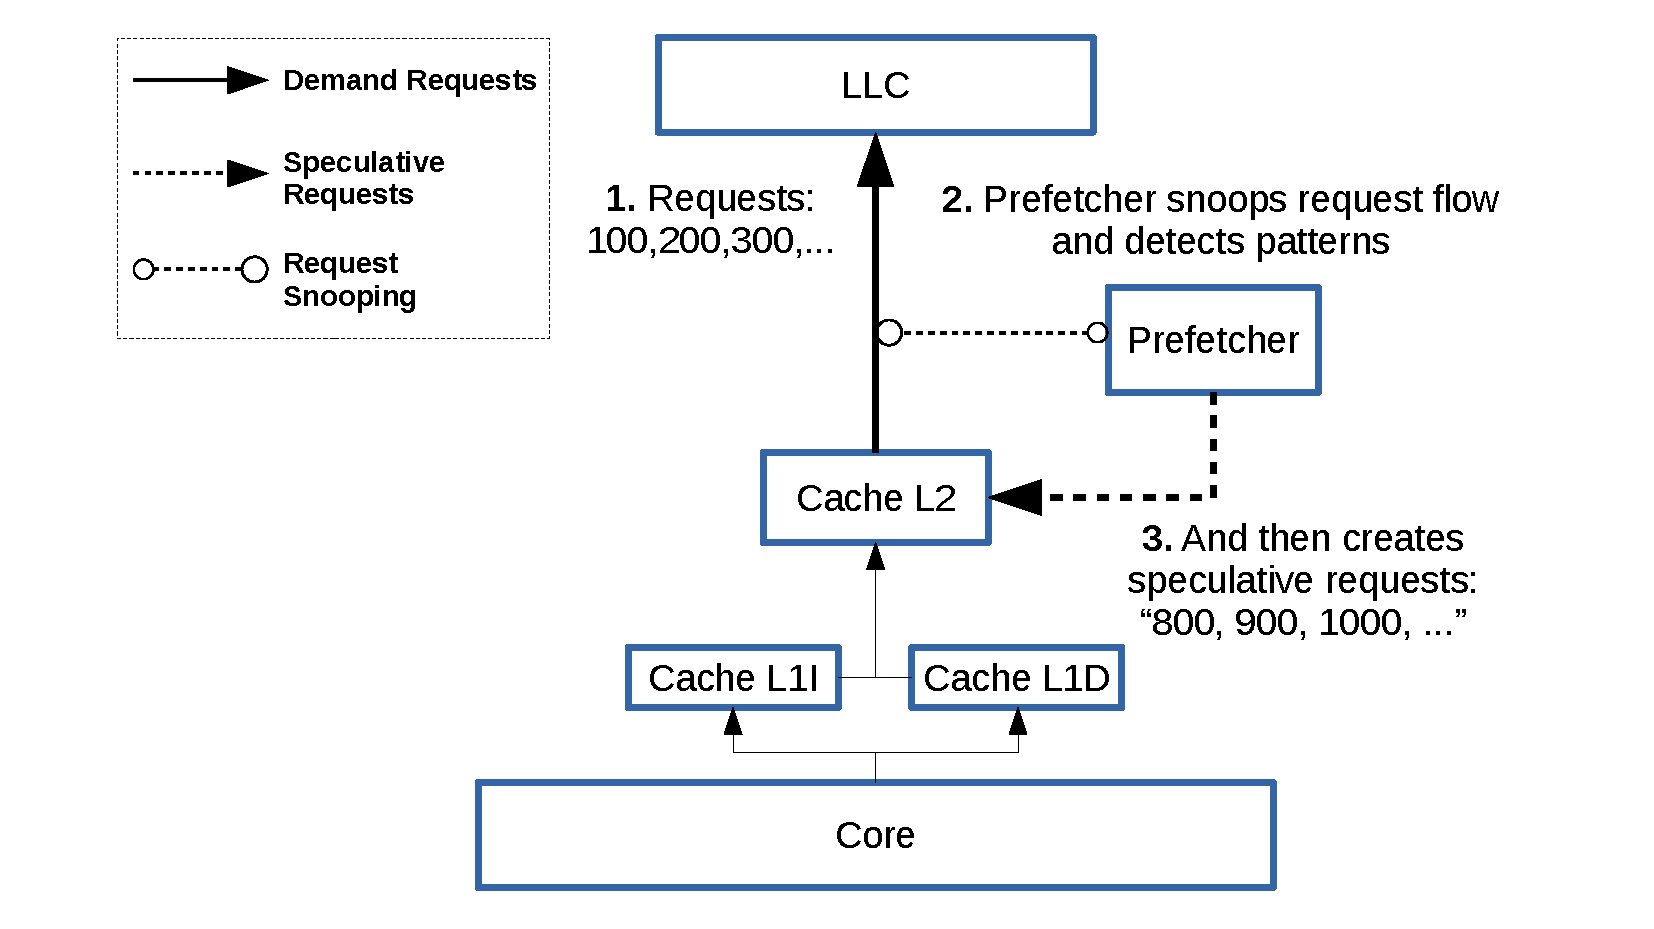
\includegraphics[width=.7\textwidth]{figures/figpref-en.pdf}
  \caption{Abstraction of the prefetcher behavior.}
  \label{fig:prefetcher}
\end{figure*}

Figure \ref{fig:prefetcher} shows an example of a second level of cache (L2) prefetcher detecting a stride access pattern.
The L2 cache forwards requests to the LLC (shown in Figure \ref{fig:prefetcher} as the event \textbf{1}).
The prefetcher, in turn, intercepts these requests by snooping the cache interconnection (\textbf{2}) and identifies the access pattern being generated.
Based on the pattern identified, speculative accesses are inserted into the L2 Miss Status Holding Register (MSHR) (\textbf{3}), a buffer that keeps track of miss events that still need to be handled.
These speculative requests are made directly to the L2 cache in order to avoid a redundant cache fill if the speculated line already resides in the cache.
These accesses are seen as regular requests made to the L2 by the prefetcher, so the L2 does not actually need to forward the response to the L1.
If the speculated address is not present in the L2 yet, the next levels in the hierarchy will forward the response to whoever requested it, as in a regular access.
%so it will eventually be received by the L2 when a L2 miss occurs and it requests the prefetch to its next level.
Thus, when the processor needs the data requested by prefetch, it will already be at a closer cache level (in this case, the L2 cache).



\subsection{Simulators}

In computer architecture research, physical implementation and analysis are infeasible due to the complexity and high cost for manufacture. 
Consequently, architecture simulators are considered the primary mechanism to implement and evaluate a new ideas in this research field.
In High-Performance Computing (HPC) systems, there are many other problems besides those inherent to the architecture.
To develop and analyze new ideas that attenuate problems arising from parallelism, we require multicore architecture simulators that support parallel workloads.
For example, in systems with dozens of cores, problems such as the interference among the different threads and the communication costs among them must be modeled to obtain accurate results.
Thread interactions occur mainly through shared memory, with several threads accessing the same memory addresses, making necessary to keep data coherence in the several cache levels.
Thereby, parallel simulators must provide an accurate implementation of cache coherence protocols and ensure data consistency through the memory hierarchy.


In the following subsections, we present the two simulators used in this work, ZSim\cite{sanchez2013zsim} and Sniper\cite{carlson2014aeohmcm}.

\subsubsection{ZSim}\label{ref:subs_zsim}

ZSim was selected for our study due to its speed and accuracy, characteristics presented in its validation study~\cite{ZSim2016validation}.
It is an instruction-driven simulator that uses dynamic binary translation (DBT) to perform the instruction execution and dynamic instrumentation.
The simulation uses a two-phase method called Bound and Weave.
In the Bound phase, a few thousand cycles are simulated, ignoring the contention and applying a minimal latency for all memory accesses.
In this phase, a trace of all memory accesses is recorded, including which caches lines were accessed, evicted, invalidated, and so on.
In the Weave phase, a parallel simulation is performed, oriented to the events of the recorded interval to determine the actual latency of each memory request in each component.
Once the interactions between memory accesses have already been identified in the first phase, this timing simulation of these accesses can be done efficiently, maintaining high precision.

The authors observed that, in an interval of a few thousand cycles, most of the concurrent accesses between different cores happen to unrelated cache lines.
Therefore, simulating these unrelated accesses first out of order and ignoring contention and, later, simulating them in order respecting time constraints, is equivalent to simulating them entirely in order.
However, when accesses are related, i.e., access the same cache line, it is necessary to maintain the coherence of the different copies of the data in the different cores.
An example of this is when a core demands exclusive access over a shared cache line to write into it, causing the cache coherence protocol to invalidate the other copies of the line in the cache hierarchy system.

The set of requests and messages necessary to invalidate the other copies of the line to obtain it as exclusive is known as Request for Ownership - RFO.
However, for being considered rare, the order of these accesses to the same line is not modeled by ZSim, which can change the path of this data in the cache hierarchy.
Changing the path of the data through the cache can impact the number of cycles, misses, and coherence messages observed in the simulation.
In addition, the generation and the paths of prefetch requests can also change, preventing the modeling of prefetcher in this simulation model.

In its validation, ZSim uses the benchmark PARSEC \cite{bienia2008parsec} and only shows that the speed-up is close to that obtained with real executions by varying the number of threads.
Therefore, as the prefetcher is not simulated, we seek to understand the impact of its absence and evaluate the accuracy of the Bound and Weave method used to simulate multiple structures and threads in parallel. 

\subsubsection{Sniper}
\label{subsubsec:sniper}

Sniper is a simulator that extends the original interval simulation model~\cite{genbrugge2010interval} to improve its handling of overlapping memory accesses through a more detailed dependency analysis of memory accesses~\cite{carlson2014aeohmcm}.
The simulator presents the instruction-window centric (IW-centric) simulation model, a high-level core model that combines the interval modeling with a detailed simulation model of the instruction window, or reorder buffer (ROB)~\cite{carlson2014aeohmcm}.
%The simulator presents the instruction-window centric (IW-centric) simulation model, a high-level core model that combines the interval modeling with a detailed simulation model of the instruction window, or reorder buffer (ROB).
%This methodology is called instruction-window centric (IW-centric) simulation.
The IW-centric simulation model focuses on accurately simulating the parallelism and latencies of instructions' execution in the processor. 
This is done by modeling micro-op dependency and issue timing in detail, estimating the performance by processing micro-ops out of order, in a way similar to how a real processor would issue them~\cite{carlson2014aeohmcm}.
However, the IW-centric model requires a longer simulation time.
For that reason, in this study we make use of their improved interval simulation model.

% eu tinha falado do IW-centric model, enquanto que nos nossos experimentos a gente usou o interval model deles, então vou reescrever
%Sniper works with a structure as big as the ROB of the architecture being simulated. 
%Each dispatched micro-op is contained in this structure and is waiting the results of the operations on which they depend. 
%As the results are completed, additional micro-ops are issued to each functional unit, potentially out of order. 
%Therefore, the complexity of the issue logic increases as the size of a processor’s ROB grows.
%Additionally, the IW-centric model needs to monitor all input dependencies of each micro-op, with the cost of potentially checking micro-ops multiple times during their lifetime. %\fbm{tu viu o codigo pra afirmar isso?}
%\vsg{nao, tudo isso que eu afirmei aqui ta no artigo de validacao deles (https://dl.acm.org/doi/10.1145/2629677)}


The basis for interval analysis is the observation that, in the absence of miss events such as branch mispredictions and cache misses, a well-balanced superscalar out-of-order processor should smoothly stream instructions through its pipelines, buffers, and functional units~\cite{eyerman2009model}. 
Under ideal conditions the processor sustains a level of performance (instructions per cycle) roughly equal to the superscalar dispatch bandwidth~\cite{eyerman2009model}. %\fbm{NOPE. Nope, nope. eh "equal to" algo, mas com certeza nao eh superscalar dispatch bandwidth. Falta uma referencia nessa frase tb, n sei de q artigo tiraste essa informacao}
%\vsg{citei esse artigo acima que e justamente o citado no artigo do sniper }
However, the smooth dispatch of instructions is intermittently disrupted by memory request miss events and branch mispredictions. %\fbm{faltou branch mispred, oq complica a historia 1 pouco}
%\vsg{nao entendi o que tu quis dizer aqui}
The effects of these events at the dispatch stage divide execution time into intervals, and these intervals serve as the fundamental entity for analysis and modeling\cite{eyerman2009model}.
The original interval modeling is itself a simulation model that allows the simulation of prefetchers in Sniper.
%fbm: não fica clara a ligacao desse therefore, alem de ser repetitivo com a primeira frase do paragrafo

The interval simulation works with two structures named new window and old window.
Each window contains as many micro-ops as would exist in the reorder buffer (ROB) of an out-of-order processor~\cite{carlson2014aeohmcm}.
The new window represents the upcoming micro-ops and is fully filled the entire time, and the old window contains a list of the most recently dispatched micro-ops~\cite{carlson2014aeohmcm}.
%In the absence of miss events, such as long-latency loads, the ILP exposed by the ROB of an out-of-order processor will determine the current performance of the core (along with the core’s maximum dispatch width).
The instantaneous IPC is calculated as the number of micro-ops in the entire old window divided by the latency of the micro-ops on the critical path~\cite{carlson2014aeohmcm}.
By repeating this process for each micro-op (and accumulating the leftover work for future micro-ops), Sniper can estimate the application’s instruction level parallelism (ILP) during the non penalty portion of an interval~\cite{carlson2014aeohmcm}.




In its validation, Sniper uses the benchmark SPLASH-2\cite{woo1995splash} and also shows that the average speed-up error is small when varying the number of threads.
%https://users.elis.ugent.be/~leeckhou/papers/ispass2019-sniper-arm.pdf
%
Although Sniper provides an implementation of the prefetcher's behavior, it has only been recently validated for the Cortex-A53 and Cortex-A72 ARM cores~\cite{adileh2019racing}.
The prefetcher model is responsible for over half of the simulation error in the \emph{povray} and \emph{x264} benchmarks, as some implementation details of the real hardware are unknown.
However, the validation used only sequential benchmarks.
In contrast, this study contributes to a better understanding of the accuracy of the simulated prefetch model and how it behaves in simulations of parallel architectures.




\section{Related Work}\label{sec:related}
%\ms{francis melhora o RW?}
%\fbm{revisado, aceito sugestoes para melhoras. colocar coisas +recentes e relacionadas a prefetcher talvez?}


Due to the lack of explicit information that hardware companies employ to avoid competition and breaches of their intellectual property, it is difficult to obtain an accurate simulation that correctly presents all the characteristics of a processor and its architecture. 
Therefore, designers of a simulator seek a low relative error when validating their simulator, and tailor the details of the simulator to make it sensitive specifically to the desired area of design, e.g., memory hierarchy~\cite{eeckhout2010computer}. 

For instance, if we variate the amount of cache memory and try to simulate a target program that requires a large amount of cache memory, the simulator should indicate loss or gain of performance. 
If it does not, either it does not model the cache correctly or suffers from bottlenecks in other parts of the model.%, preventing the application's sensitivity to memory access from transpiring. 

\subsection{Improving Simulator Accuracy}

Microbenchmarks can be used to decrease error in basic architecture structures and as a form of reverse engineering of architectural features~\cite{fog2012microarchitecture}.
%\ms{reviewer's head: why these guys talk about it and not use in their own work?}\fbm{great question :P allow me counter: we are interested in parallel benchmarks and measuring "prefetcher with communication" accuracy in the models, and I do not picture a microbenchmark doing that. maybe r2 stuff}
%\ms{what I mean is whether the previous paragraph is a tiro no pe or not}\fbm{it's old stuff done for single core. I'd say it's just mandatory citation when talking about simulator accuracy, since Desikan }.
In Desikan et al.'s work~\cite{desikan2001measuring}, the authors faced the difficulty of obtaining accurate information and studied the relevance of this information when validating the SimpleScalar simulator~\cite{austin2002simplescalar}. 
By obtaining more information about the Alpha 21264 processor model in direct contact with the manufacturers, the authors were able to reduce the experimental microbenchmarks error from 19.5\% to 2\%.  
With the SPEC-CPU 2000 workload, the average experimental error went from 36.7\% to 18.2\%. 
The authors then showed how the resources found generate bottlenecks in different parts of the system than previously modeled in several articles, invalidating ideas that presented performance gains due to bottlenecks that did not exist.
%\fbm{I feel like mentioning they had to do an errata and apologize to that paper LOL} %\cite{desikanerrata}

A more recent work by Walker et al.~\cite{walker2018hardware} in this direction automates the process of finding the source of simulator error.
The main objective of the work is to obtain more accurate energy consumption models for gem5, but to do so they required a more accurate processor model. 
Using gem5 and the processor configurations provided by Gutierrez et al.'s gem5 validation~\cite{gutierrez2014sources}, Walker et al. created GemStone, a framework to find the sources of simulation error based on empirical hardware performance monitor counters (PMCs) models.
%\ms{at this point, I expect (at the end of this section) a very convincing story of why our paper should be accepted}.
GemStone selects the events in gem5, correlating them with the PMC events, and at last, performs one regression analysis to approximate the relationship between hardware PMCs and gem5 error, and another to approximate the relationship between gem5 events and gem5 error.

%In their work, an hierarchical cluster aggregation (HCA) was used to cluster workloads from MiBench, ParMiBench, PARSEC, Dhrystone, and Whetstone (45 in total) accordingly to the values of the given PMCs.
%They observe that workloads in the same cluster, i.e. similar values for their events, had similar Mean Percentage Error (MPE), thus correlating the MPE to the type of workload.
%They then use HCA to cluster PMC events that correlate with each other across the workloads, finding that inter-process communication cost is too low, while branch misprediction rates are too high due to many instruction translation lookaside buffer (ITLB) misses.
%Afterwards, GemStone selects the events in gem5, correlating them with the PMC events, and at last, performs one regression analysis to approximate the relationship between hardware PMCs and gem5 error, and another to approximate the relationship between gem5 events and gem5 error.
%They find 8 events that model the error with $R^{2} = 0.99$ and adjusted $R^{2} = 0.99$, confirming the hypothesis regarding branches (which had a smaller correlation) causing the frequent ITLB misses.
%GemStone also automatically identified other possible sources of error in these events, such as the data translation lookaside buffer (DTLB) prefetch faults.
%In summary, GemStone is a promising framework to reduce simulation error, but so far it's only available for gem5.
%\fbm{n sei como, mas tem q dar 1 tiro neles... o paper tem mt erro gramatical, mas a ideia eh solida, vao perguntar pq n usamos gem5. also, tem q cortar 1 pouco desses paragrafos, se alguem tiver sugestoes...}\ms{eu cortaria esse paragrafo inteiro}



\subsection{Prefetcher Simulation}

The development of new prefetching techniques is an active area.
%\ms{I suggest split the related work into subsections -- simulators -- prefetch -- motivation}
Mittal~\cite{mittal2016survey} provides a survey on recent development of prefetching techniques up to 2016.
In the survey, the authors describe the relevant prefetch metrics, such as accuracy, coverage, and timeliness~\cite{srinath2007feedback}, as well as the different types of technique to improve prefetching, such as new pattern detection techniques~\cite{nesbit2004data}, filtering prefetches~\cite{zhuang2006reducing}, dropping prefetches~\cite{lee2008prefetcher}, changing prefetches' priority on the memory controller~\cite{ebrahimi2009coordinated}, and so on.
Given the variety of techniques and the active development of new techniques, one can hardly keep up with the design of prefetchers and additional techniques in the industry, which are not publicly disclosed.
Thus, most simulator designers face difficulties when modeling prefetchers, as they cannot real hardware information.
Interestingly, many of these techniques are not tested in multithreaded applications, where communication plays a major role in the memory hierarchy latency~\cite{jain2018rethinking,wu2019efficient,bhatia2019perceptron}, which we explore in this work.

\subsection{Simulator Survey} 

Since Desikan's work, several simulators have been created along a validation effort to evaluate their accuracy.
%\ms{fiquei ou ficou confuso - os caras que tao propondo o simulador tao mostrando o erro eh isso?}\fbm{eh exatamente isso}.
In Akram et al's research~\cite{akram2019survey}, the authors evaluated and compared the gem5~\cite{binkert2011gem5}, Multi2Sim~\cite{ubal2012multi2sim}, MARSSx86~\cite{patel2011marss}, PTLsim~\cite{yourst2007ptlsim}, Sniper~\cite{carlson2014aeohmcm}, and ZSim~\cite{sanchez2013zsim} simulators. 
After thorough characterization of the simulators, the authors tested single core and multiprogrammed workloads on each simulator. 
The results of each simulator were compared with the Intel's Haswell architecture~\cite{hammarlund2014haswell}. 
The authors then highlighted the error sources of the simulators, their sensitivity to different architectural parameters, and their relative error. 
Thus, they concluded that the lack of validation of a simulator for the target architecture, no matter how popular it is (e.g., gem5, which was only validated for ARM~\cite{gutierrez2014sources}), leads to low accuracy and may render experiments invalid due to erroneous conclusions.

However, Akram's work does not use multi-thread applications to verify the error relative to the number of threads and the accuracy of communication in these simulators.
The two best simulators in Akram's results, in terms of accuracy, were Zsim and Sniper, which we selected for this work.
%\ms{applications? some works use the term multi-thread workloads as multiple multithreaded applications running at the same time}
%\ms{um pouco deslocado esse paragrafo}



%\subsection{Discussion and Motivation}

%We are interested in parallel benchmarks and measuring the ``prefetcher with communication'' accuracy in the models, which has not been analyzed in any of the previous works.
%To do so, we evaluate and compare hardware counters and simulator events related to the prefetchers, pointing out the sources of inaccuracy in the prefetcher modeling, such as the lack of aggressive adaptability or prefetch filtering/dropping, which has been reported by Intel~\cite{intelmanual}.
%\fbm{vou adicionar algo coerente assim q terminar de passar por todo o paper :P}


\section{Methodology and Experimental Environment}\label{sec:experiments}
%We are interested in parallel benchmarks and measuring the ``prefetcher with communication'' accuracy in the models, which has not been analyzed in any of the previous works.
%To do so, we evaluate and compare hardware counters and simulator events related to the prefetchers, pointing out the sources of inaccuracy in the prefetcher modeling, such as the lack of aggressive adaptability or prefetch filtering/dropping, which has been reported by Intel~\cite{intelmanual}.
In this Section, we present details about the experimental environment and the prefetcher algorithms provided by the real machine hardware and by Sniper.
Moreover, we describe the methodology applied in the experiments, the benchmark used and the different prefetcher combinations executed and simulated.


%\subsection{Experimental Workflow}
\subsection{Experimental Setup}
\label{subsec:exp-setup}
%\vsg{melhorar titulos}


\begin{table}[b]
    \centering
    \footnotesize
    \caption{Real machine, ZSim and Sniper configurations.}
    \label{tablehb}
    \renewcommand{\tabcolsep}{1pt}
   % \newcolumntype{L}[1]{>{\raggedright\let\newline\\\arraybackslash\hspace{0pt}}m{#1}}
   
   \resizebox{.8\linewidth}{!}{
    \begin{tabular}{{@{\hspace{0.0cm}} l @{\hspace{0.1cm}} @{\hspace{0.1cm}} c @{\hspace{0.1cm}} @{\hspace{0.1cm}} c @{\hspace{0.1cm}} @{\hspace{0.1cm}} c
    @{\hspace{0.1cm}} @{\hspace{0.1cm}} c @{\hspace{0.1cm}} @{\hspace{0.1cm}}}}
    \toprule
    & \bfseries Real &\bfseries ZSim  &\bfseries Sniper \\
    \midrule
    Processor Frequency & 2.1 Ghz & 2.1 Ghz  & 2.1 Ghz \\ 

    Number of Cores & 12 & 12  &  12 \\

    Pipeline Stages & 18 & 16  &  16\\

%    Busca de Instruções & 16B & 16B  \\
    
%    Fila de Instruções & 18 & \textbf{NA} \\
    
%    Decodificação Paralela & até 5 uops & até 5 uops \\
    
%    Buffer de Decodificação & 56 & 28 \\
    
%    \emph{cache} de uops & 1536 uops & \textbf{NA} \\ 
    
%    Renomeação & 4 uops & 4 uops \\
    
%    Estações de Reserva & 54 & 36 \\
    
%    Execução  & até 6 uops & até 5 uops \\
    
%    Buffer de Reordenamento & 168 & 128 \\
    
%    Buffer de Leitura & 32 & 32 \\
    
%    Buffer de Escrita & 16 & 32 \\
    
%    Graduação Paralela & 4 & 5 \\
   
 %   \midrule
 %   Preditor de Desvios & Tournament  & 2-level PAg \\
    
 %   Penalidade & 15-20 & 17 \\
    
    \midrule
    Cache Line Size & 64~B & 64~B  & 64~B\\
    
	L1 Data Cache & 8-way 32~KB & 8-way 32~KB  & 8-way 32~KB\\
	
	Latency & 4 & 4  & 4\\
    \midrule
    
    L1 Instruction Cache & 8-way 32~KB & 8-way 32~KB  & 8-way 32~KB\\
	
	Latency & 4 & 4  & 4 \\
    \midrule
    
	Unified L2 Cache & 16-way 1~MB & 16-way 1~MB  & 16-way 1~MB\\
    
    Latency & ca. 14 & 14 & 14\\
    \midrule
    
    Last Level Cache L3 & Non-inclusive 11-way 16.5 MB & Inclusive 11-way 16.5~MB  & Inclusive 11-way 16.5 MB\\
    
    Latency & ca. 60-80 & 77 & 77\\
    \midrule
    Prefetchers & L1 IP Stride &  & Simple (Stride L1 Prefetcher)\\
                & Adjacent Line prefetcher & No Prefetcher & Global History Buffer  \\
                & L2 DCU Stream prefetcher & & (L2 Prefetcher)  \\
    \bottomrule
    \end{tabular}
    }
\end{table}


% msserpa: quando vir mintor colocamos a tabela dos hardware counters. agora pode dar mais motivo para os revisores
\new{To collect information about the application execution in the real machine, we make use of the PAPI~\cite{terpstra2010papi} tool.
PAPI allows the obtaining of hardware counters values, a set of registers that provide information about CPU events such as the number of instructions and the number of cycles.
In each real execution, only one hardware counter is evaluated, thus avoiding aggregations or approximations that the tool performs when calculating several metrics in the same execution.}
The performance and the real executions statistics were evaluated with 10 executions of each metric, for each benchmark.
The execution environment was composed of an Intel Xeon Silver 4116 CPU \textbf{with 2.1 GHz of frequency}, the Skylake microarchitecture~\cite{doweck2017skylake}.
The simulation environment is an approximation of the real hardware, respecting the simulators' limitations.
Each simulation was executed only once, and all statistics were extracted from the same simulation.
\textbf{All the executions in the real machine were performed with the Intel Turbo Boost~\cite{rotem2012turbo} technology disabled.}

%\ms{falar da cache non-inclusive. que esse processador eh. e o que significa isso}.
\textbf{An important observation regarding Skylake's architecture is the change from an inclusive L3 cache to a non-inclusive one.
Skylake's predecessor architecture was Intel Broadwell, which applies an inclusive L3 cache, meaning that all data brought into the L2 cache is also brought into the LLC.
However, in non-inclusive L3 caches like the one used by Skylake, the data found at the L2 cache may or may not be found in the LLC, and there is no guarantee regarding how it will behave.
Which data is brought to which level depends on the application's access pattern, code and data sizes and their layout in the memory, and also on the inter-thread communication and sharing behavior.
}


%\ms{nao sei se aquele 2.1 - 3 GHz eh necessario... so pra botarem minhoca. E se eh pela realidade eh na verdade 0.8 - 3 GHz o correto}
Table~\ref{tablehb}  presents the configuration of the real machine and the processor simulated by ZSim and Sniper. 
The Sniper's out of order core model was based on the Nehalem architecture~\cite{carlson2011sniper}, while ZSim based its out of order core model implementation on the Westmere architecture~\cite{sanchez2013zsim}, a process shrink of Nehalem.
Therefore, both simulators present a 16 stages pipeline, while the real machine architecture may present between 14 and 19 stages~\cite{fog2012microarchitecture}.
Other parameters such as cache associativity and cache access latency are easy to configure in the simulators and can be found in~\cite{fog2012microarchitecture,doweck2017skylake}.



%\ms{qual fonte de 11way na L3?}
%\vsg{pag da skylake no wikichip}
%\ms{okkk}

%informações sobre os prefetchers agora: citar os prefetchers que são apresentados no optimization manual https://en.wikichip.org/w/images/d/d0/intel-ref-248966-040.pdf
In Table~\ref{prefetches}, we present the description of the prefetcher algorithms considered in this work. 
The algorithms found in the L1 cache hardware are the Data Cache Unit (DCU) Prefetcher~\cite{intelmanual} and the DCU IP Prefetcher~\cite{intelmanual}.
The DCU Prefetcher, also known as the streaming prefetcher, is triggered by an ascending access to very recently loaded data. 
The processor assumes that this access is part of a streaming algorithm and automatically fetches the next line.
The DCU IP Prefetcher keeps track of individual load instructions (based on their instruction pointer's value). 
If a load instruction is detected to have a regular stride, then a prefetch is sent to the next address which is the sum of the current address and the stride.


The L2 Hardware Prefetcher~\cite{intelmanual} and the L2 Adjacent Cache Prefetcher~\cite{intelmanual} are the prefetcher algorithms found in the real machine L2 cache.
The L2 Hardware Prefetcher monitors read requests from the L1 cache for ascending and descending sequences of addresses. 
Monitored read requests include L1 data cache requests initiated by load and store operations and also by the L1 prefetchers, and L1 instruction cache requests for code fetch.
When a forward or backward stream of requests is detected, the anticipated cache lines are prefetched.
This prefetcher may issue two prefetch requests on every L2 lookup and run up to 20 lines ahead of the load request. 
The L2 Adjacent Cache Prefetcher fetches two 64-byte cache lines into a 128-byte sector instead of only one, regardless of whether the additional cache line has been requested or not.

The prefetcher algorithms in Sniper are the Simple and the Global History Buffer (GHB)~\cite{nesbit2004data}.
Based on an analysis of the Simple prefetcher's code, we observed that it is similar to a strided prefetcher algorithm.
Thus, we use the Simple prefetcher as the L1 cache prefetcher in our experiments.
The GHB prefetcher is an $n$-entry FIFO table that holds the $n$ most recent L2 misses addresses. 
Each GHB entry stores a global miss address and a link pointer that is used to chain the GHB entries into address lists. 
Each address list is a time-ordered sequence of addresses issued by the same instruction pointer.
Therefore, based on the information of the address lists, it is possible to implement a correlation based prefetcher~\cite{charney1995GeneralizedCB} and a stride prefetcher~\cite{nesbit2004data}.
The L2 prefetcher found in Sniper is a GHB correlation based prefetcher, and in our experiments it is used as the L2 cache prefetcher.


Therefore, based on the aforementioned prefetchers, we conducted experiments on the real machine considering: \textcolor{red}{\textbf{ATUALIZAR AQUI QUANDO OS GRÁFICOS NOVOS EM R ESTIVEREM PRONTOS!!!!}}
\begin{itemize}
    \item All Skylake's L1 cache prefetchers, henceforth "Real-L1 prefetcher", or simply L1 prefetcher;
    \item All Skylake's L2 cache prefetchers, henceforth "Real-L2 prefetcher", or simply L2 prefetcher;
    \item All Skylake's prefetchers from both L1 and L2 cache, henceforth "Real-L1-L2 prefetcher", or simply L1+L2 prefetcher;
    \item No prefetcher, henceforth referred to as Real-No Prefetcher.
\end{itemize}

Based on the Sniper's prefetchers, the following systems were simulated:
\begin{itemize}
    \item Only the L2 data prefetcher (GHB), henceforth "Sniper-L2 prefetcher", or simply Sniper's L2 prefetcher;
    \item Both L1 (Simple) and L2 (GHB) prefetchers, henceforth "Sniper-L1-L2 prefetcher", or simply Sniper's L1+L2 prefetcher;
    \item No prefetcher, henceforth referred to as Sniper-No Prefetcher.
\end{itemize}

Since ZSim does not model the prefetcher behavior, there are no variations of the simulated system. With ZSim we only perform simulations with no prefetcher, which we refer to as ZSim.

%comentar tbm que o modelo de simulação usado no sniper é o interval e tbm falar dos modelos de prefetcher que tão disponíveis e quais foram usados

\vsg{tabela com os counters que foram utilziados e os significados (Matheus)}



\begin{table}[]
    \centering
    \footnotesize
    \caption{Prefetcher algorithms.}
    \label{prefetches}
\resizebox{1.0\linewidth}{!}{
\begin{tabular}{@{}c|c|c|c|c|c@{}}
\toprule
\textbf{}                 & \textbf{Description}                                                           & \textbf{L1} & \textbf{L2} & \textbf{Real} &  \textbf{Sniper  } \\ \midrule
DCU Prefetcher   & %Prefetch of next L1 Data line based upon multiple loads in the same cache line 
Streaming prefetcher, fetches the next cache line into L1-D Cache  & \checkmark 
&   & \checkmark  &       \\
DCU IP Prefetcher         & 
Strided prefetcher of next L1-D line based upon sequential load history & \checkmark & & \checkmark  &       \\
%Uses sequential load history to prefetch additional lines into L1-D Cache                    
%& teste &  & \\
L2 Hardware Prefetcher       & Mid Level Cache (L2) streamer prefetcher                                       &             & \checkmark  & \checkmark  &                \\
   L2 Adjacent Cache Prefetcher & Prefetching of adjacent cache lines into L2 Cache                                          &             & \checkmark & \checkmark  &                  \\
%LLC Prefetch              & Last Level Cache  prefetching on all threads
% (hardware cache) &             &             \\ \bottomrule
Simple & Strided prefetcher of L1-D line & \checkmark &  & & \checkmark \\ 
Global History Buffer & L2 Prefetcher based on global miss addresses & & \checkmark & & \checkmark \\
\end{tabular}
}
\end{table}

 

\subsection{NAS Parallel Benchmarks}
\label{subsec:nas}

\vsg{botar so o significado das siglas}

For this study, we used a known HPC benchmark in the literature called Numerical Aerodynamic Simulation Parallel Benchmark (NPB)~\cite{jin1999openmp}. 
\new{This set of applications comprises ten applications, each of which encapsulates a certain type of computation that is often processed by HPC applications, e.g. computational fluid dynamics (CFD), adaptive meshes, parallel I/O, and computational grids.
We used nine of the ten NPB applications, namely: CG, EP, FT, IS, MG, UA, BT, LU, and SP.
The Data Cube (DC) application was discarded because DC mainly stresses I/O operations, which are not modeled by the architecture simulators.}


%\textbf{TODO EXPLICAR NA CARTA} 
\new{The benchmark set presents different input classes that offer different input sizes and complexities.
The available input classes are: S, W, A, B, C, D, E, and F.
The class S was designed for quick testing purposes; class W was originally designed for standard testing considering a 90's workstations, and nowadays is used for quick test purposes as well; classes A, B, and C are standard test problems, whose size increases four times from one class to another; and classes D, E, and F, for large-size problems, whose size increases sixteen times from one to another.}


%\fbm{ficou incoerente o uso de ; entre itens dada as descricoes grandes deles, seria bom reformatar acho}
%\textcolor{blue}{\textbf{DCS: In the list of items please use the standard of “;” after each item and “.” at the final one}}
%Para a avaliação de escalabilidade do erro relativo ao número de \emph{threads}, foi usado o \emph{benchmark} \emph{Numerical Aerodynamic Simulation Parallel} \emph{Benchmarks} (NPB)~\mbox{\cite{jin1999openmp}}.
%Este \emph{benchmark} é composto por dez aplicações paralelas, das quais nove foram usadas.
%As aplicações utilizadas neste trabalho são:

%\iffalse % comentário
%\vspace{-1mm}
\begin{comment}
\begin{itemize}

\item \textbf{CG}: \emph{Conjugate Gradient} uses a conjugate gradient method to approximate the smallest eigenvalue of a defined, large and sparse, symmetric matrix. 
This application tests for irregular memory accesses and long-distance communication between threads, employing matrix multiplication by a structureless vector;

%utiliza um método de gradiente conjugado para aproximar o valor do menor autovalor de uma matriz simétrica positiva definida, grande e esparsa. Este \emph{kernel} testa comunicação de longa distância irregular, empregando multiplicação de matriz por vetor sem estrutura.
\item \textbf{EP}: \emph{Embarrassingly Parallel} solves the problem of generating pairs of Gaussians and tabulating their values in successive annuli squares. 
Unlike the other NPB applications, EP has virtually no communication, only stressing the performance of floating-point operations;

%resolve o problema de gerar pares de gaussianas e tabular seus valores em quadrados \emph{annuli} sucessivos. Ao contrário do resto da lista, este \emph{kernel} praticamente não possui comunicação, estressando apenas o desempenho de operações de ponto flutuante.
\item \textbf{FT}: \emph{Fourier Transform} solves the problem of the three-dimensional Fourier transform in a parallel way using the Fast Fourier Transform (FFT) algorithm. FT strictly tests high-distance communication with an all-to-all core communication pattern;

%resolve o problema da transformada de Fourier tridimensional de forma paralela usando o algoritmo de transformada rápida de Fourier (FFT). Testa rigorosamente a comunicação de alta distância, ocorrendo comunicação de todos \emph{cores} com todos \emph{cores}. 
\item \textbf{IS}: \emph{Integer Sort} uses Bucket Sort to sort a vector of integer numbers. 
IS has random memory accesses and tests both the integer operations performance and communication;

%resolve o problema de ordenar inteiros usando \emph{bucket sort}. Possui acessos randômicos à memória, e testa tanto o desempenho de operações com inteiros quanto a comunicação.
\item \textbf{MG}: \emph{Multigrid} solves a simplified multi-grid calculation problem by testing short- and long-distance communications. 
MG requires highly structured long-distance communication;

%resolve um problema simplificado de cálculo \emph{multigrid}, testando comunicações de curta e longa distâncias. Requer comunicação de longa distância altamente estruturada.
\item \textbf{UA}: \emph{Unstructured Adaptive Mesh} solves a problem of heat transfer in a cubic domain, discretized in an unstructured adaptive mesh;

%resolve um problema estilizado de transferência de calor em um domínio cúbico, discretizado em uma malha sem estrutura refinada adaptativamente.
\item \textbf{BT}: \emph{Block Tridiagonal} solves a synthetic Computational Fluid Dynamics (CFD) problem with multiple 5x5 tridiagonal block equation systems with non-dominant diagonals. BT has more limited parallelism than other CFD applications (LU and SP);

%resolve um problema sintético de CFD com múltiplos sistemas de equações de blocos tridiagonais 5x5 com diagonais não-dominantes. Tem paralelismo mais limitado que os outros CFD (LU e SP).
\item \textbf{LU}: \emph{Lower Upper Gauss-Seidel Solver} solves a synthetic CFD problem by solving a system of sparse triangular linear equations, with 5x5 blocks. LU involves global data dependencies, with several short communications;

%resolve um problema sintético de CFD ao resolver um sistema de equações lineares triangulares esparsas, com blocos de 5x5. Envolve dependências de dados globais, com várias comunicações curtas.
\item \textbf{SP}: \emph{Scalar Pentadiagonal} solves systems of pentadiagonal scalar equations with non-dominant diagonals. 
Like LU, SP involves global data dependencies, though with more infrequent and longer communications.

%resolve sistemas de equações escalares pentadiagonais com diagonais não-dominantes. 
%Assim como o LU, envolve dependências de dados globais, mas com comunicações mais infrequentes e mais longas.
\end{itemize}

\end{comment}


%fbm feito até aqui




%\section{Results and Performance Analysis}\label{sec:results}
%\subsection{Real Machine Execution}
%\label{subsubsec:real_ipc}
\section{Investigating Current Architecture Prefetchers}\label{sec:real_ipc}

In this section, we present the main results obtained by the aforementioned experimental setup, taking into account the real execution of the NPB benchmark. 
More specifically, here we shed light to the following question: \new{\textit{How do the different prefetchers affect the execution of NPB over a real machine with a varying level of parallelism?}}
%\fbm{"behave" is quite vague. basically, what we are answering is "how do the presence of prefetchers affect the execution of NPB under a different number of threads"}
% Please add the following required packages to your document preamble:
% \usepackage{booktabs}


%EP is a special case in NAS, so it deserves special attention
%\subsubsection{Embarrassingly Parallel - EP}
%\subsubsection{Prefetcher Metrics}

%In Figure~\ref{epfig}, we illustrate the characteristics of the Embarrassingly Parallel (EP) benchmark.
%Subfigure (a) shows the instruction per cycle (IPC) of the application according to the number of executing threads.
%Since the EP benchmark is known to not make much use of memory, little contention occurs during execution, and thus the IPC is stable for any number of threads on all cores.
%Therefore, there is also little difference in the IPC given different prefetcher configurations, as prefetches are not exploited by the EP application.
%msserpa inverti a ordem de umas palavras aqui

%In Subfigure(b), we can observe the total number of read prefetches that reached the offcore caches during the EP execution.
%An interesting observation is that, although L1+L2 prefetchers should generate more requests, EP has an unpredictable behavior, where for certain numbers of threads, the L2 prefetcher alone creates more offcore requests.
%As explained in the methodology Section~\ref{sec:experiments}, Perf counts these hardware events in a system-wide fashion.
%Therefore, other applications generate noise on EP's prefetcher metrics, which distorts the relation between the prefetches generated by the different configurations.

%When examining the total number of 

%\fbm{essa parte deveria ser jogada fora? oq aconteceu aqui q tem uma ref meio perdida de subfig?}

%This is due to the fact that the L1 prefetcher can generate noise in the L2 prefetcher; if the L1 prefetcher obtains a line that prevents an L1 miss, this makes the L2 prefetcher unable to keep track of the access pattern in that page, and thus it will not generate a prefetch since it did not receive that specific access.

%- prefetcher metrics (quais?) reads, read hit


%\subsubsection{NPB Processing Performance}
%\label{subsubsec:real_ipc}
%- L2 não perde mt para L1+L2, e é mais transparente/simples.
%- ipc
%As we can see in the previous section, each prefetcher has distinct characteristics according to the evaluated metrics. Though, surprisingly, the efficiency of executing NPB with some prefetchers is similar.
Figure~\ref{fig:ipc} shows the instructions per cycle (IPC) for each NPB application, using the input class A, taking into account different numbers of threads and prefetchers, and with hardware prefetcher disabled as well. 
The IPC can be understood as a general performance metric of the prefetchers when executing the applications, since an efficient prefetcher will enable more processed instructions per cycle \new{by fetching the right data at the right time}. 
The error bars represent the variability observed among both the cores of a certain execution and the 10 distinct repetitions of the executions.
%\ms{tem que ajustar os plots pra se algum revisor imprimir conseguir ler e tal...}
%\ms{podia ter uma tabela antes dos resultados explicando os contadores e metricas usadas}
%\vsg{sem mt tempo e sem mt espaco}

\begin{figure}[b]
    \centering
    %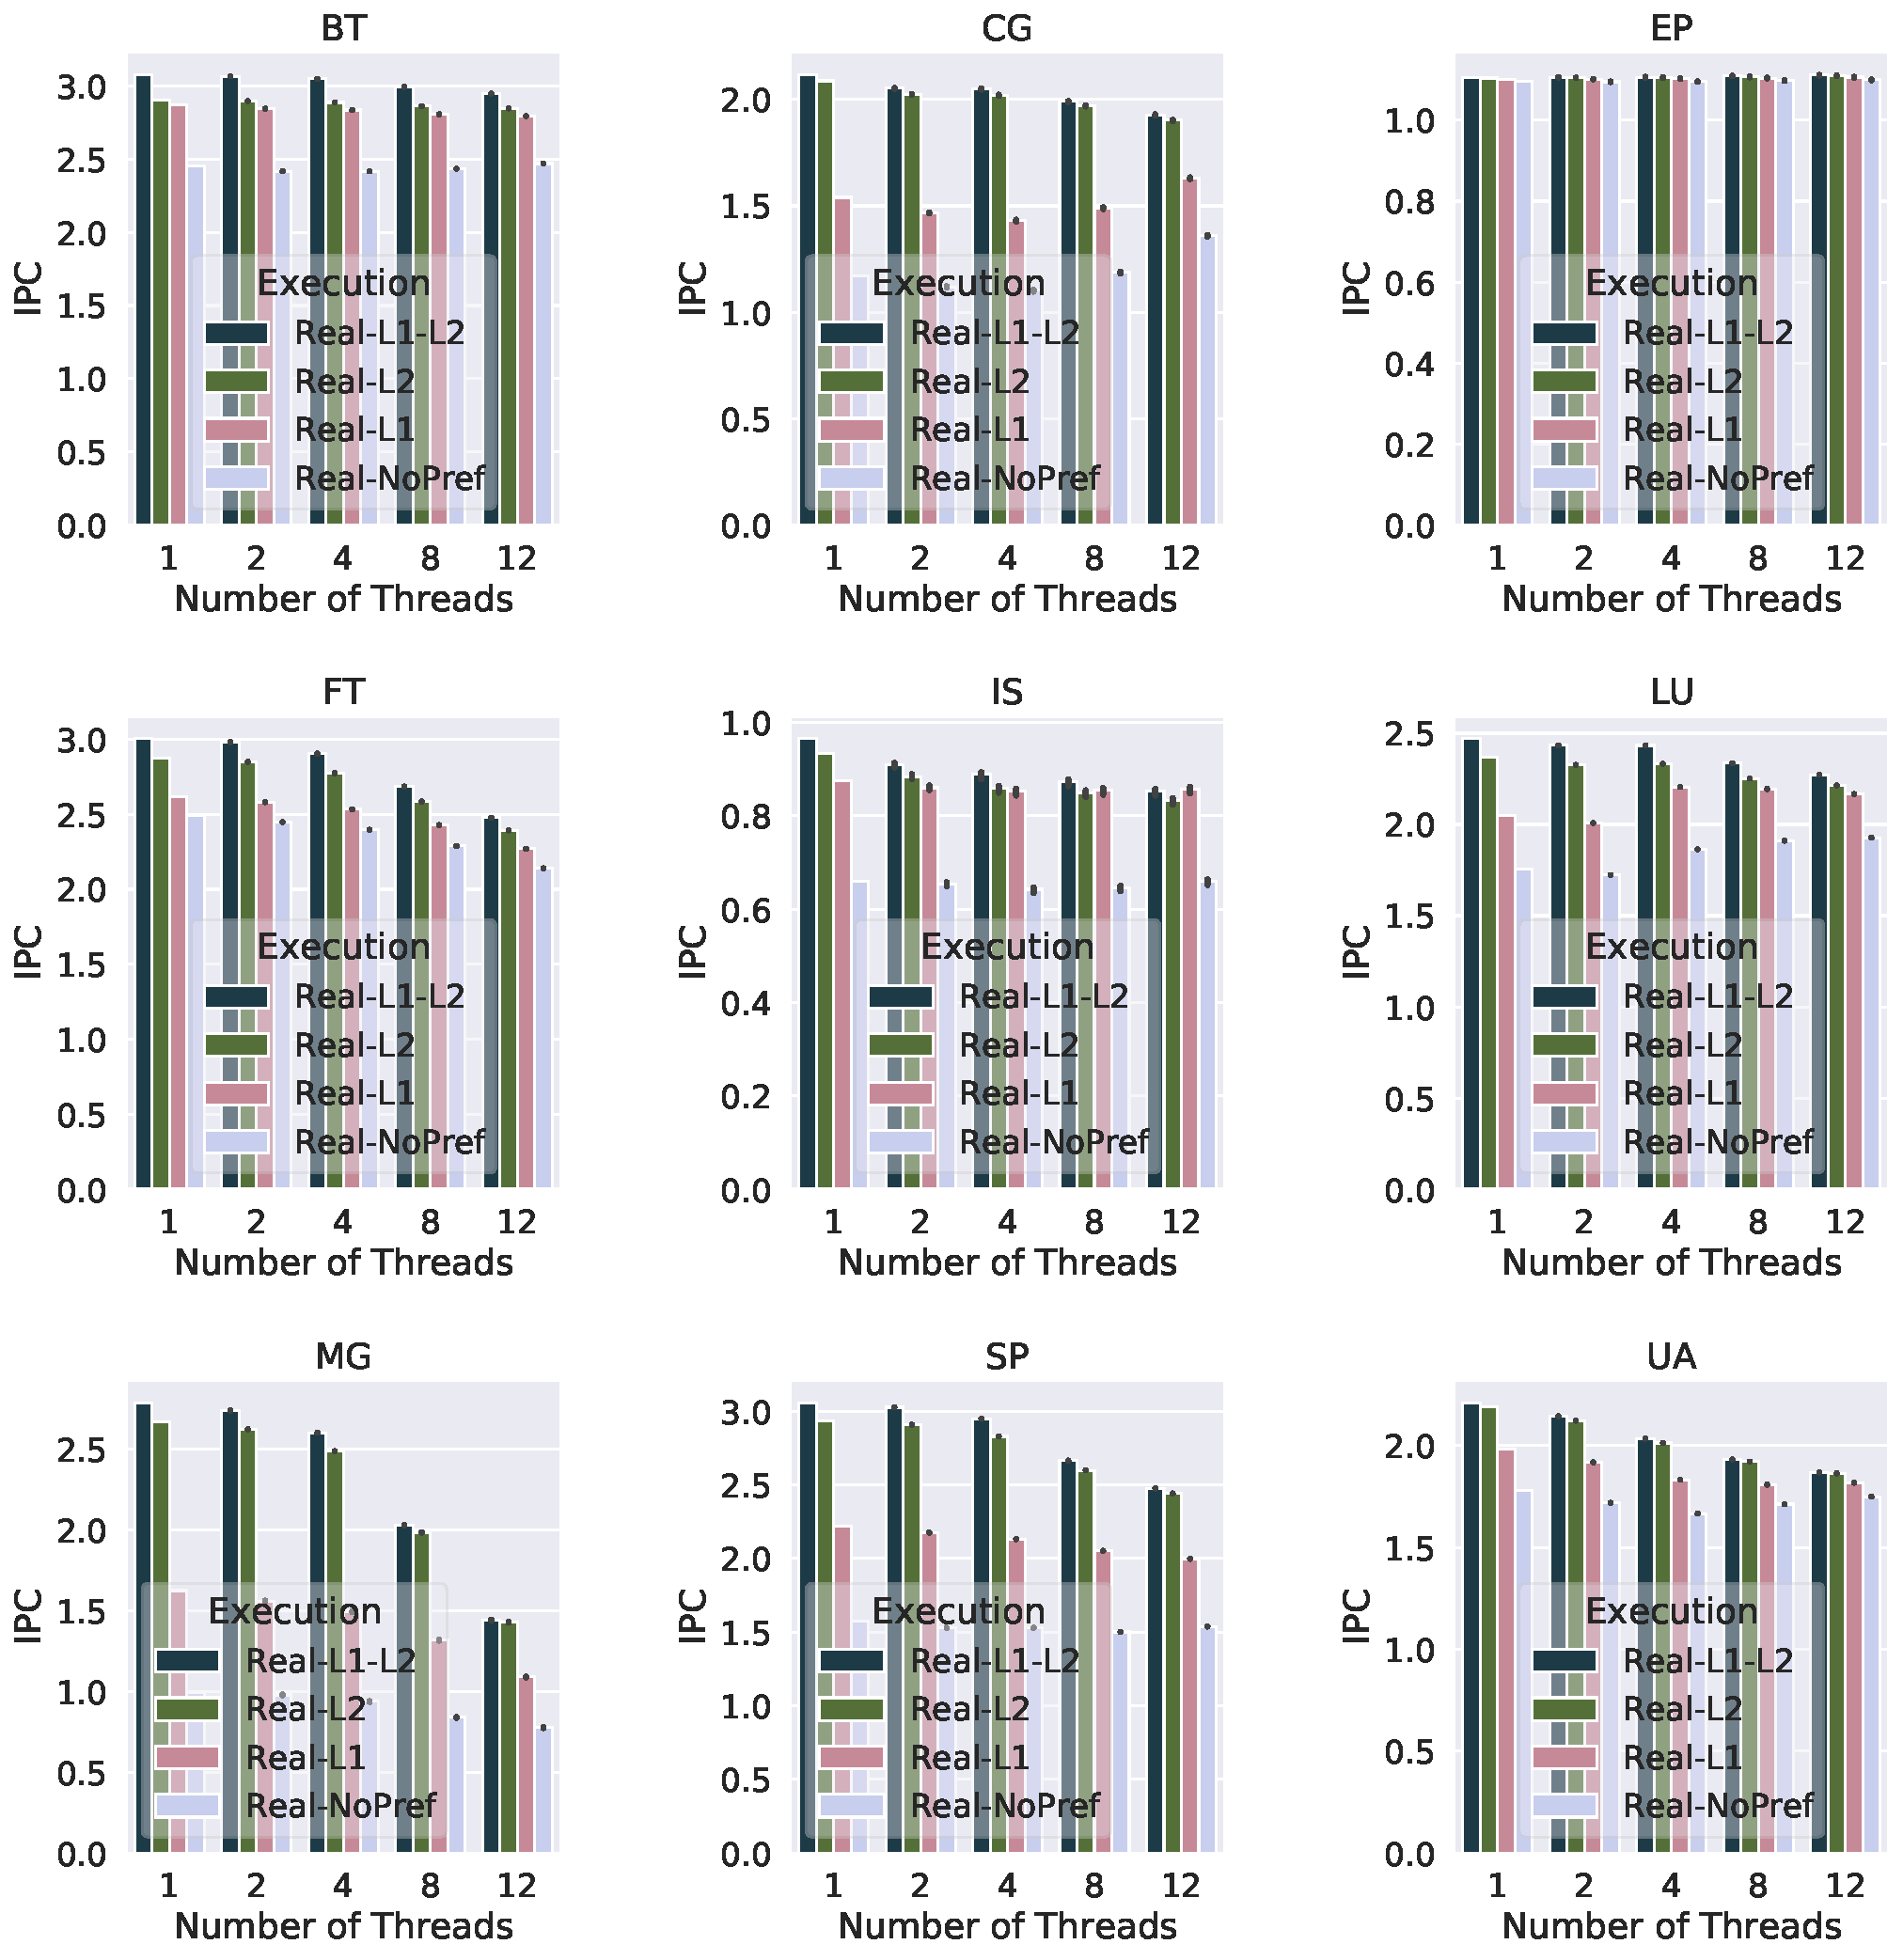
\includegraphics[width=.8\linewidth]{figures/IPC_A_all_subm2_cei_noturbo.pdf}
    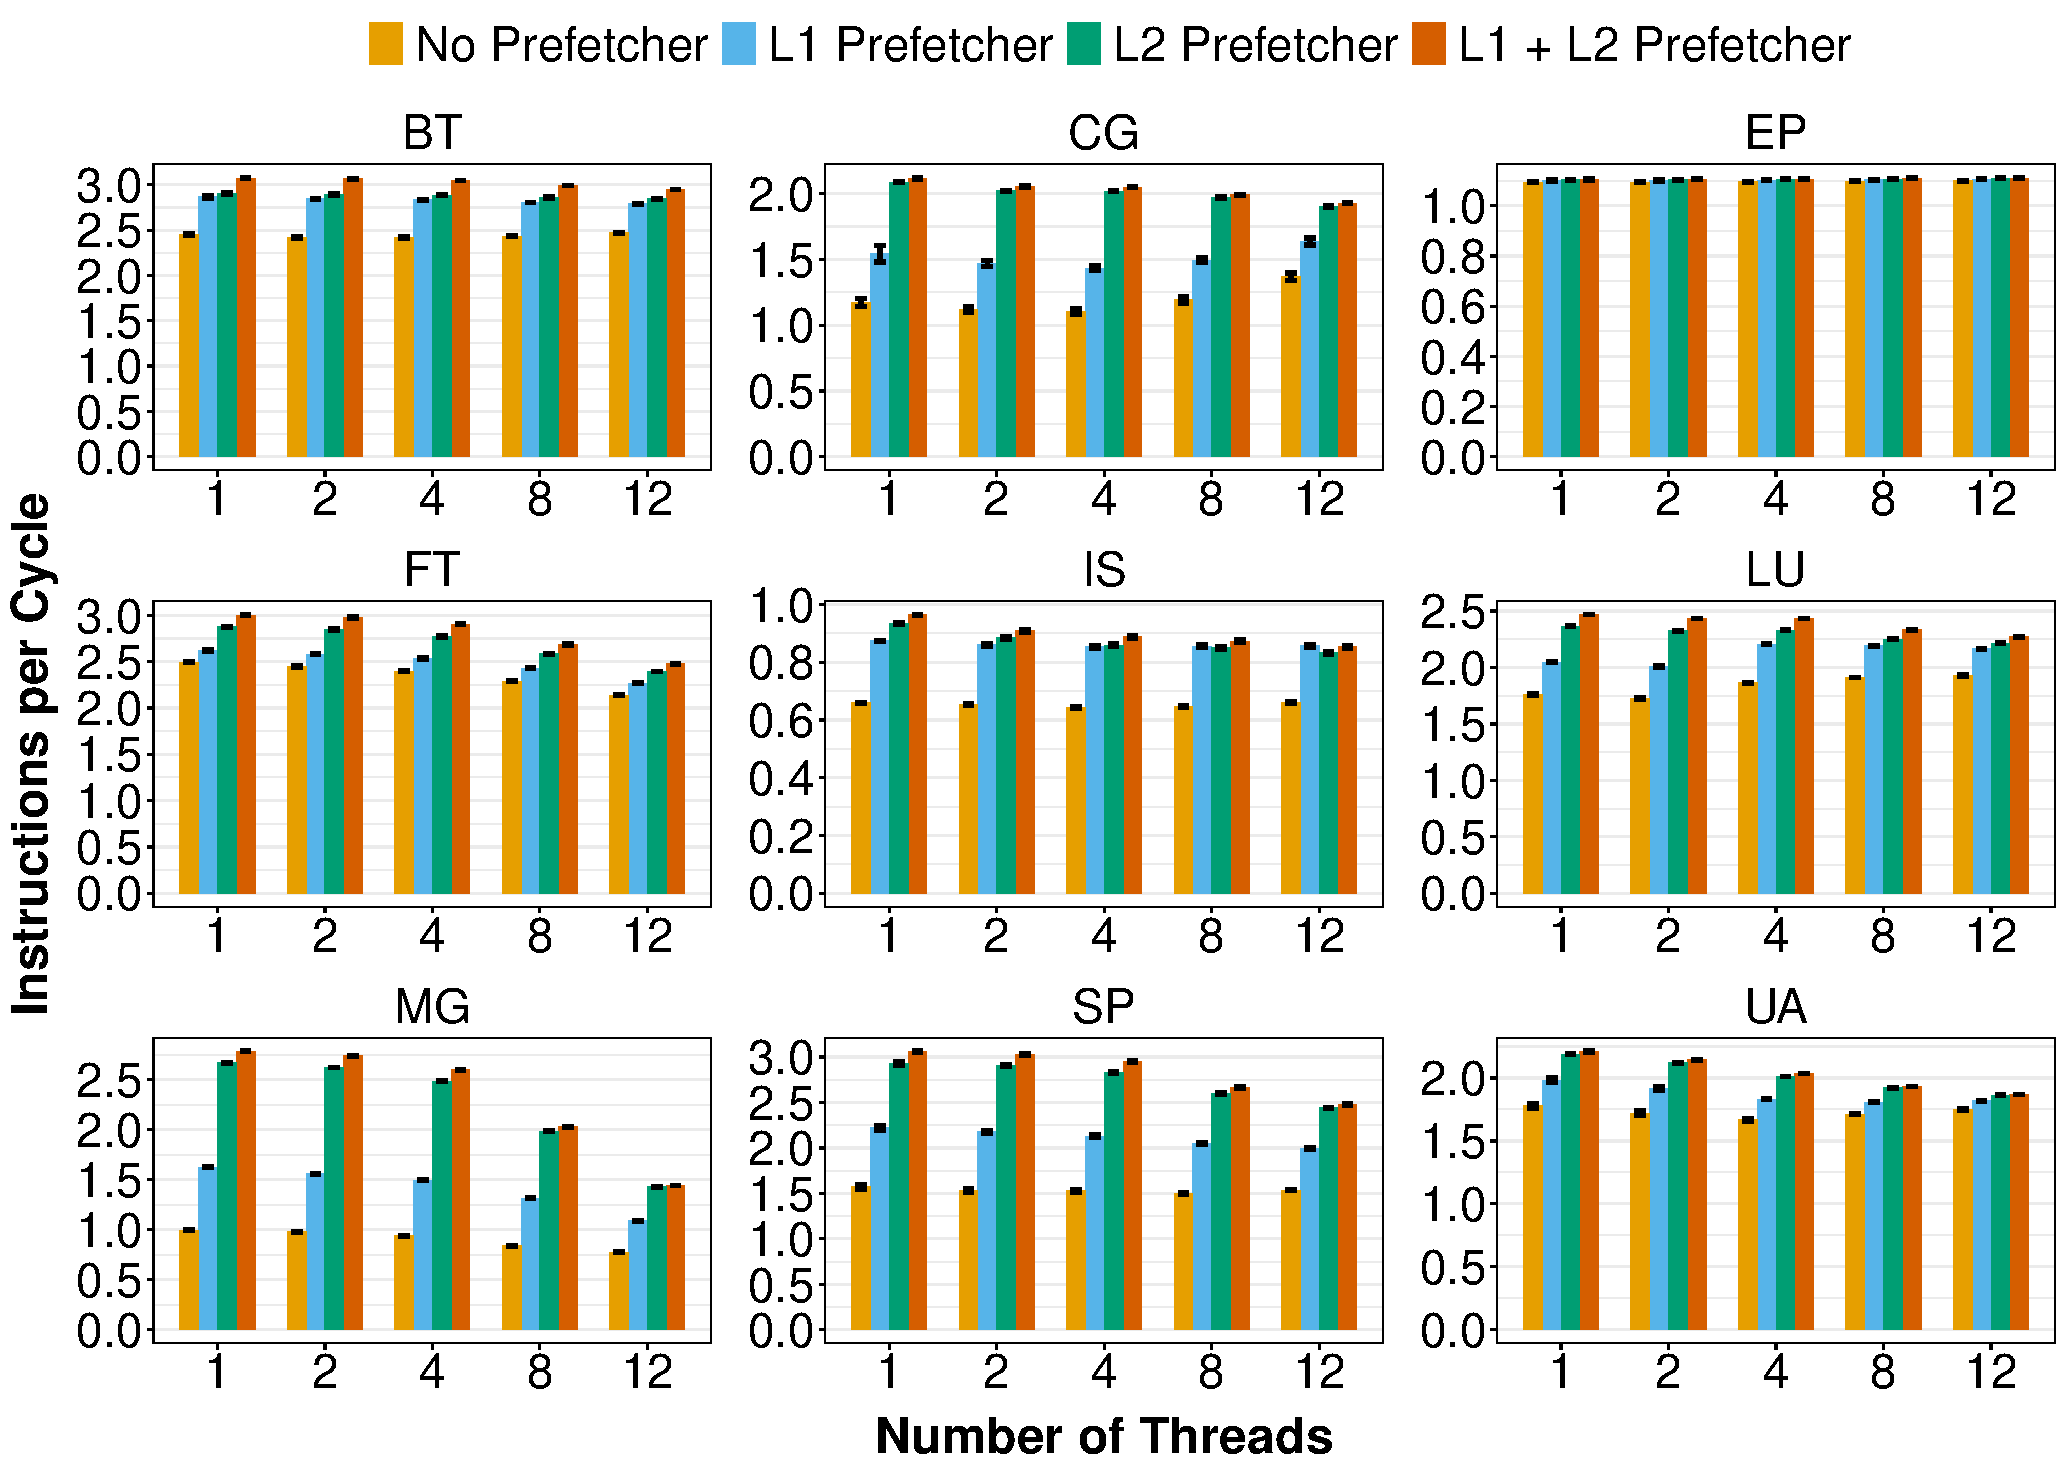
\includegraphics[width=\linewidth]{figures/fig2.pdf}
    \caption{IPC results for the real execution of the NPB applications with input class A.}
    \label{fig:ipc}
\end{figure}

% citar como o prefetcher funciona (meio que lembrando do que é falado sobre o prefethcer na seção do prefetcher): o pref funciona desse jeito, então por isso é natural termos ganho em performance
As expected, we can observe that any prefetcher increases the execution performance of NPB, with the exception of the EP application. 
Since EP is known to have a small memory footprint~\cite{jin1999openmp}, processor stalls due to memory access latency rarely occur during its execution. 
Therefore, there is little difference in the IPC given different prefetcher configurations for EP. 
For the other applications, memory prefetching significantly contributes to a better IPC, specially for executions up to four threads.


However, the increase in performance from a standalone L2 prefetcher to the combination of L1+L2 prefetchers is not as large, with an overall average IPC improvement of 3.3\%, when compared to the performance increase from no prefetcher to the standalone L2 prefetcher. \fbm{which is..? how much does the L2 standalone increases IPC?}
\vsg{aqui Matheus}
\new{This can be explained by the L2 prefetcher's ability to detect more relevant memory access streams that are dependent on the LLC's long-latency response, while the L1 prefetcher detects access to data that might be found at the on-core L2 cache level.}
Since the difference in latency from L1 to L2 is small, and the latency from L2 to LLC is much larger, this means the main performance gains would be obtained by the L2 prefetcher and the associated access streams it detects.
For concrete numbers, the L2 cache access latency is of 14 cycles, only 10 cycles higher than the L1 cache, while the LLC latency in Skylake is measured to be approximately between 60 and 80 processor cycles, presenting a much more substantial overhead and a higher probability of stalling the processor execution~\cite{alves2015sinuca}. 
\new{Furthermore, in Figure~\ref{fig:real_l2-rqsts-all-pf} we present the sum of all prefetch requests performed by the active prefetchers of each active core in the real execution, also for the input class A.
We can observe that, for some applications (e.g. BT, FT, SP, and some executions of LU), the number of prefetch requests performed by the L1 prefetcher is bigger than the number of requests performed by the L2 prefetcher, and, in some cases, it almost reaches the same amount of requests performed by the two prefetchers combined (the L1+L2 executions).
Despite the L1 prefetcher issuing more prefetches than the L2 prefetcher in several cases, the fewer L2 prefetches are the ones who deliver the most crucial performance gains, as seen in Figure~\ref{fig:ipc}.}

\new{Another complementary explanation for this small performance gains observed for the L1 prefetcher is that its requests may be detrimental to performance, since they may compete with demand data for the rather limited cache space on the L1 cache level.
Moreover, these prefetch requests may also occupy too many entries on the line fill buffers present in the L1 hardware, competing again for shared and limited resources with the critical demand accesses, which are more relevant for the immediate processor execution than the prefetched lines.}%\fbm{"may occupy too many entries" is a bit uncertain. I think the limited line fill buffers certainly play a part here, but there is a lot of "may" on this paragraph that makes the text feel like pure speculation}\vsg{I removed part of the "may"}

The \textbf{L1+L2} prefetcher combination is often set as the default setting in the machine configurations.
One of its main appeal is that it is the setting that provides the best performance. 
\new{However, one drawback of this approach lies in the interpretability of what is being performed by the algorithms.
The lack of understanding over the full prefetcher hierarchy behavior hinders the accurate implementation of prefetching models in architecture simulators, which will be demonstrated in detail in Section~\ref{sec:simulation}}.%\fbm{NN are not interpretable, and people still use it a lot. I'm not sure how valid this point is} \vsg{Maybe our point here was to highlight that the lack of understanding over the prefetcher hierarchy hinders the accurate implementation of a prefetcher simulation model. I rewrote it.}
%\vsg{I think is complicated to say that the L2 prefetcher is more transparent (in the same transparent meaning considered above), because simulators also have problem implementing an accurate L2 prefetcher. Something that may be more valuable to add here is the lower energy consumption by turning the L1 prefetcher off (but this also is arguable, since the most significant power consumption is originated on the long-latency off-core accesses to the DRAM). I don't like the rest of the paragraph, we need to fix it.}
%\fbm{changing to use the inter-prefetcher noise, simplicity of standalone L2, please review below}
For instance, a small detail such as the interactions between the prefetchers of each cache level (e.g., whether the L2 prefetcher considers L1 prefetches as part of the application's access stream or as prefetch requests) can cause major changes in the behavior of the memory hierarchy.
On the other hand, the L2 prefetcher in isolation provides a simpler, more transparent understanding of the prefetches performed by the algorithm, facilitating reverse engineering and reproduction/simulation of the prefetcher, with the drawback of not having the best performance.
At the light of these results, it may be advisable to set the L2 prefetcher on its own, as opposed to the L1+L2 setting, since the lack of transparency in the details of the L1 and L2 prefetcher, the L1 line fill buffer contention, and the additional energy consumption of the L1 prefetcher may not outweigh its increase in performance.

% enfatizar isso na seção 6 dando mais ênfase

%- general trend that the higher the level of parallelism, the lesser is the impact of the prefectcher in performance

Another interesting trend observed in Figure~\ref{fig:ipc} is the decrease in the IPC for increasing number of threads in the majority of applications and prefetchers, with the exception EP application.
Apart from EP -- which, for the same reasons explained above, the IPC is stable for any number of threads on all cores -- the NPB applications use memory accesses and inter-thread communications, that naturally increase in function of the total number of threads. 
With a large number of threads, these memory accesses and inter-thread communications generate contention that become a larger constraint in the IPC, and the performance provided by prefetchers becomes small or negligible. %\fbm{Non-sequitur, prefetchers should help with that. the problem is the contention for DRAM/LLC banks} 
\new{This effect can be clearly seen in the IPC graph for the MG application: MG is known to use memory-intensive operations and to be communication-intensive, largely benefiting from memory prefetchers. 
However, as the number of threads increases, the contention becomes a more considerable constraint in the IPC results, significantly harming the performance.}
% tbm focar nisso na seção 6, sobre como olhar mais pra app pode ajudar pq chega um ponto em que o prefetcher já não faz milagre

In this regard, we hypothesize that, when the number of concurrent threads executed in a processor is high, the performance benefit from memory prefetchers for applications that use intense memory and inter-thread communications is negligible. 
\new{These characteristics would need to be alleviated on the applications for memory prefetchers to be effective.} 
However, an interesting exception to this observation is the CG application's executions with the L1 prefetcher and without prefetcher (Figure~\ref{fig:ipc}), where the IPC increases in function of the number of threads. 
We explain the CG case with more details in Section~\ref{subs:cg}.

\begin{figure}[!htb]
    \centering
%    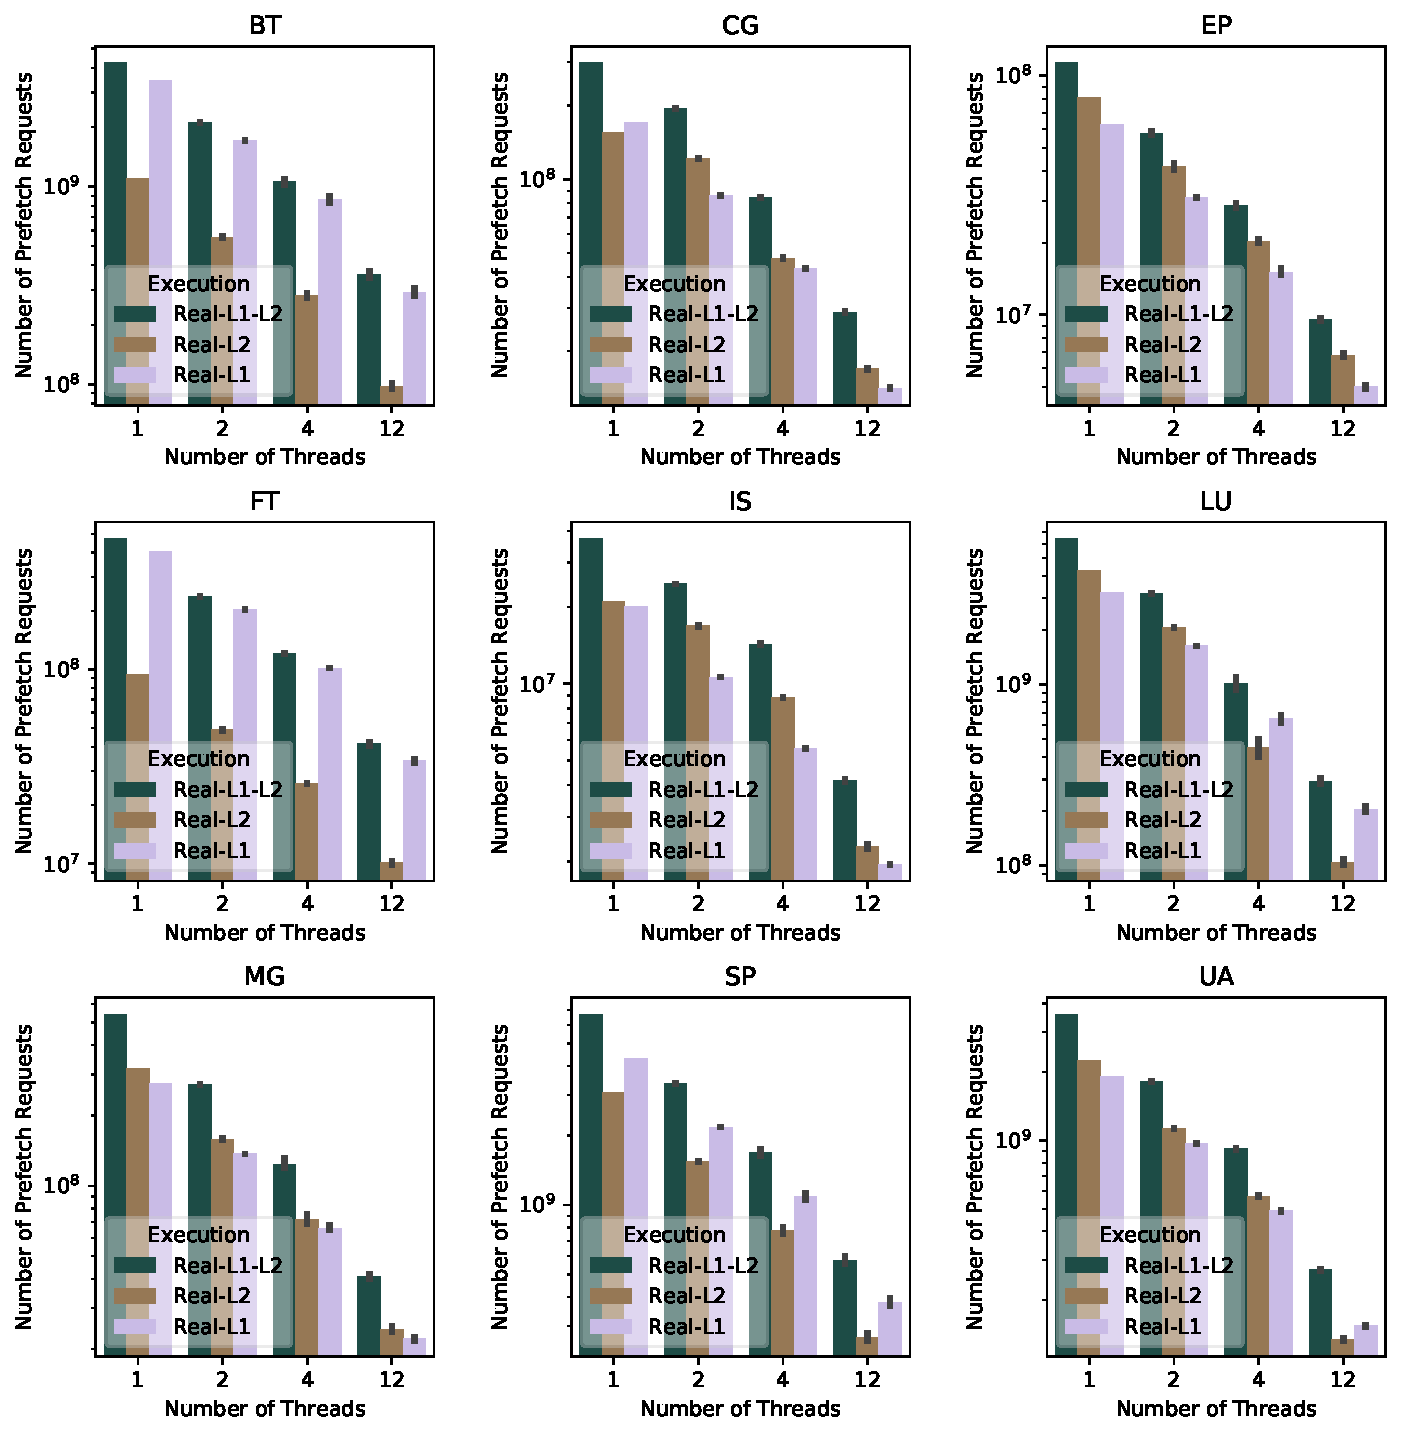
\includegraphics[width=.8\linewidth]{figures/real_l2-rqsts-all-pf.pdf}
    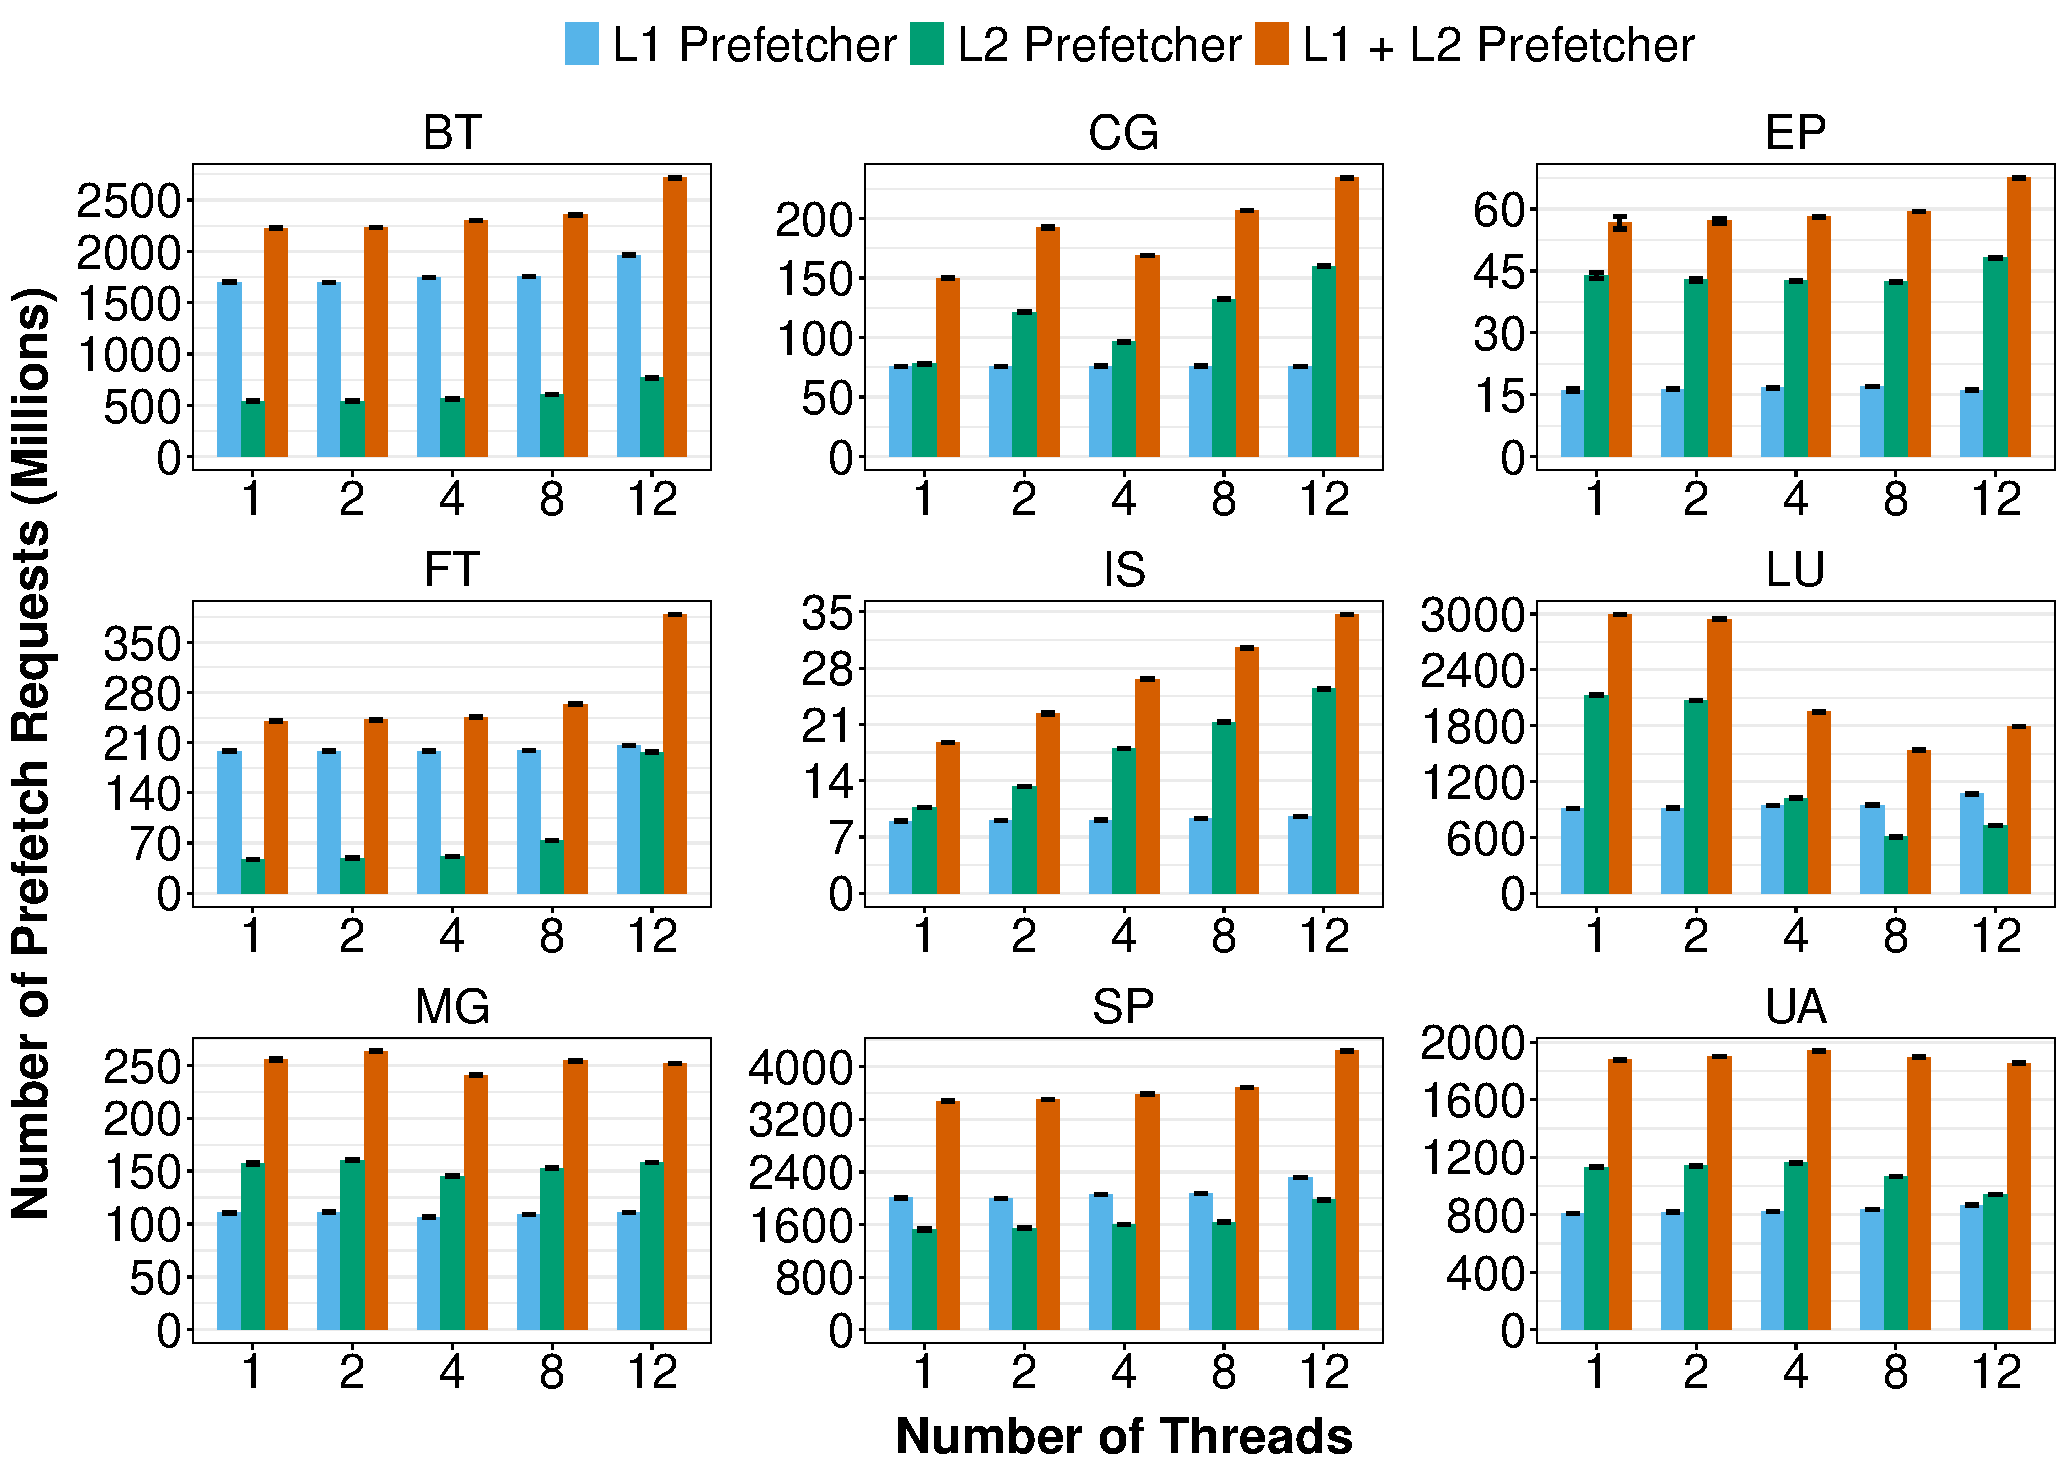
\includegraphics[width=\linewidth]{figures/fig3.pdf}
    \caption{Number of prefetch requests of the real machine executions with the input class A.}
    \label{fig:real_l2-rqsts-all-pf}
\end{figure}

%To strengthen the above hypothesis, in Figure~\ref{fig:cg_llc_miss} we show the number of LLC misses for the CG application, with input class A, in function of the number of threads, and considering no prefetcher and the L1 prefetcher.
%We can observe that the number of misses halves when we increase from 1 to 2 threads, exactly because one thread may bring data to the cache system that could be used by the other thread. 
%From 2 to 12 threads the number of LLC misses increases because, although it is more likely that the data required by a thread will be in the LLC by the effect of other thread requests, if a thread modifies this data, the cache coherency protocol will invalidate that copy of the data in the cache system.\fbm{rewrite this with the results we got}


%\textbf{francis: argumento com danilo: cada thread aumenta a cache pra working set em L2, aumentando IPC devido a melhor reuso de dados, mas conforme threads aumentam mais, ocorre contenção por uso de LLC (contenção), aumentando número de LLC misses devido a interferência inter-core}

%\vsg{a primeira premissa: prefetchers nao vao estar sendo tao preciso devido aos acessos irregulares \\ problema pq o prefetcher puxa algo que ele nao precisa mas outra thread vai poder precisar \\ tbm tem dados puxados que ninguem vai usar : poluicao \\ grafico com useless pref / num pref pra verificar a hipotese acima}



\subsection{The CG Case}\label{subs:cg}


As previously explained, all NAS applications, except CG, suffer from a performance decrease as a result of the increasing memory contention that harms the prefetcher's efficiency in highly parallel applications.
However, the CG executions with the L1 prefetcher and without prefetcher present a contrasting behavior, with the IPC increasing in function of the number of threads, as demonstrated in Figure~\ref{fig:ipc}.
This section aims to detail the CG executions to better understand the CG results, showing how the application behavior contributes to the different observations. %\fbm{"attain.." might leave a bad impression. Maybe "detail the execution of CG"?}


\begin{figure}[!htb]
    \centering
    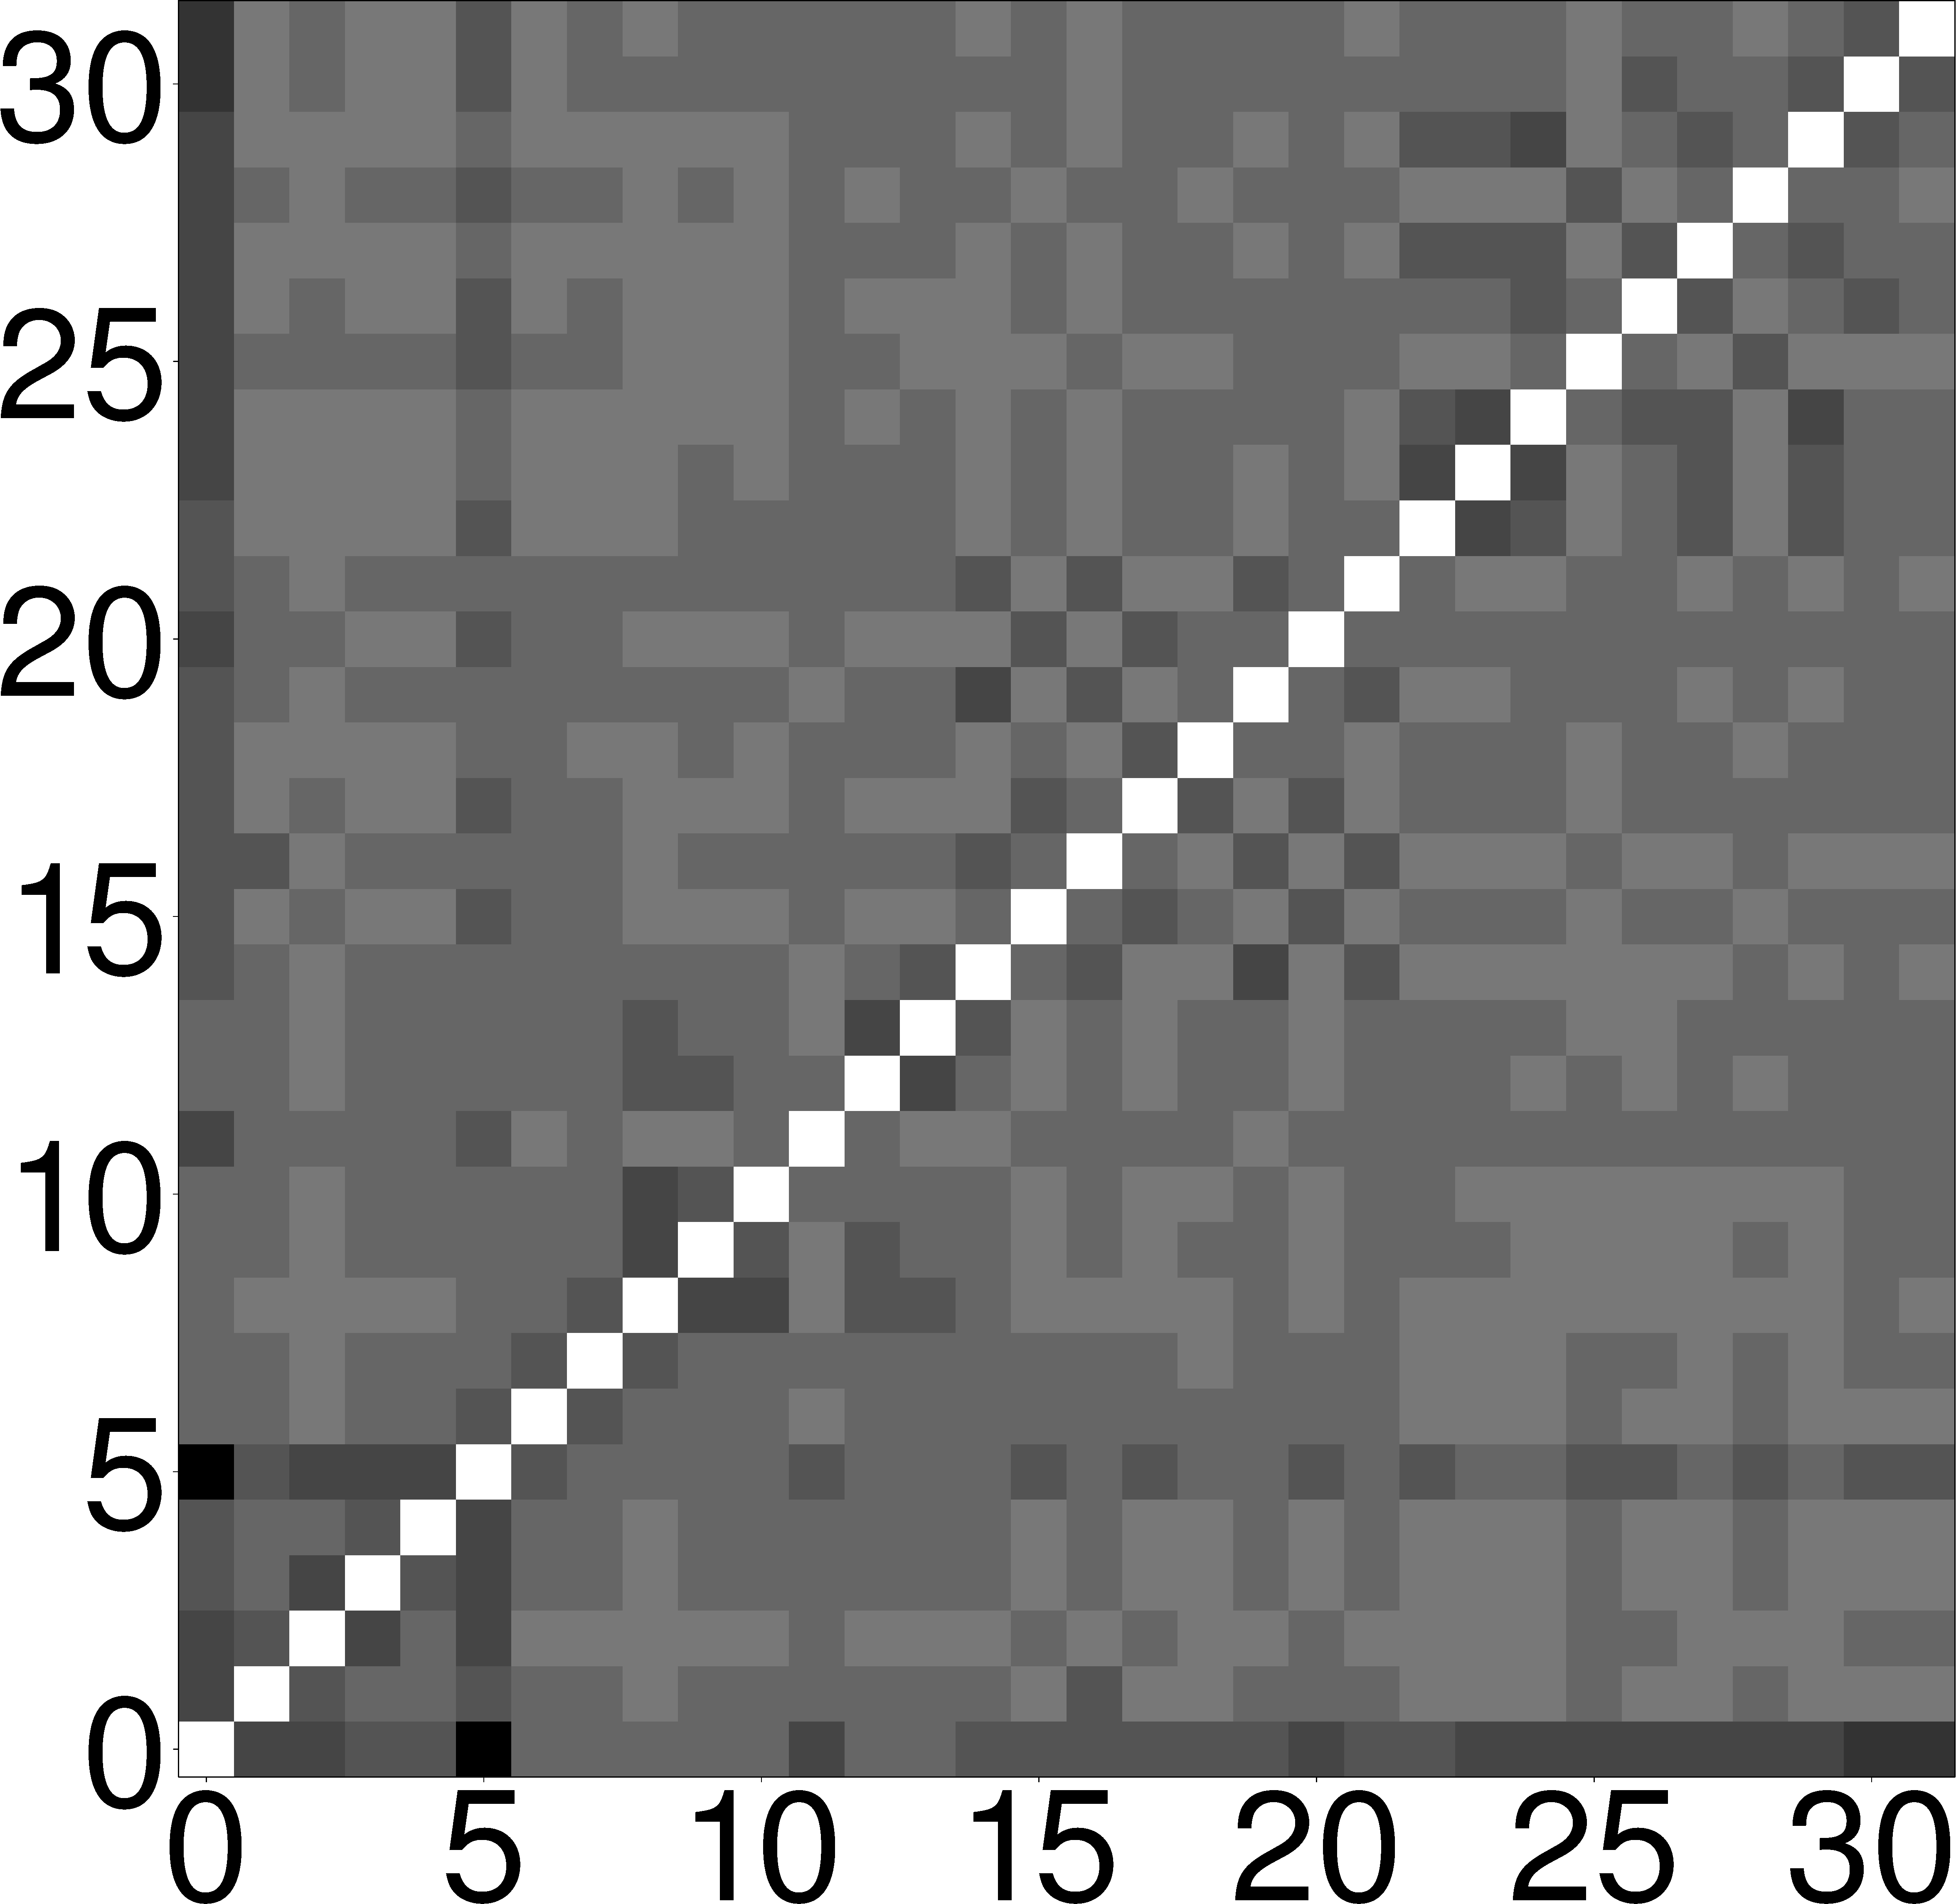
\includegraphics[width=.3\linewidth]{figures/cg.pdf}
    \caption{CG communication pattern for 32 threads. Figure obtained from: Cruz \textit{et al.}~\cite{cruz2018thread}}
    \label{fig:figcomma}
\end{figure}



First, we can observe CG's communication pattern in Figure~\ref{fig:figcomma}.
In this figure, the darker a given cell is, the more shared memory accesses occurred between the threads represented by row and column.
The diagonal is filled with white as a thread does not share data with itself.
Thus, we can see that all threads of CG irregularly communicate with all threads, as described in Section~\ref{subsec:nas}.
%This effect may be due to the irregular access nature of the CG application and its long-latency and irregular thread communication.
These irregularly distributed memory accesses enable one thread to request a memory address that had already been requested by another thread or even by another thread's prefetcher.
Since the chosen processor model has a non-inclusive L3 cache (as mentioned in Section~\ref{subsec:exp-setup}), the data found in the L2 cache is not necessarily duplicated at the L3 cache as would happen in an inclusive cache hierarchy, resulting in more available cache space.
Therefore, as we increase the number of threads, the amount of cache space available for the application is increased by using each core's private cache levels (which include an 1 MB L2 cache per core).
Consequently, a larger part of the working set of the application fits inside the processor caches, reducing the number of LLC misses, and thus reducing the number of long-latency DRAM accesses as well. 
%\fbm{"fits entirely" depends on the number of threads. Maybe we can say that "the amount of working set kept in core increases as we increase the number of threads"?}
%\vsg{explicar que o pref de insts ta ativado}


This behavior is shown in Figure~\ref{fig:drampapi}, where we depict the number of DRAM accesses as we increase the number of threads.
The instruction prefetcher has not been disabled for any of these executions, which explains the presence of prefetch requests when the hardware data prefetchers are disabled.
As we use more threads, fewer DRAM accesses need to be performed regardless of the prefetching mechanism, precisely because the application has the necessary data present in the cache.
Moreover, a more prominent decrease is observed on the demand read DRAM accesses for the executions without prefetcher.
These avoided DRAM accesses play an essential role in the performance improvements observed in these executions.
A prefetcher is accurate if it can hide the main memory latency by effectively pulling data from the main memory to cache memory before a demand access requests the data.
An accurate prefetcher should also generate a number of prefetches similar to the number of demand requests generated by the processor without prefetchers, i.e., the actual number of load/write instructions that would require data.
Otherwise, it is generating unnecessary main memory accesses to bring data that will not be used.
This does not necessarily reduce the IPC, but it can increase main memory contention, energy consumption, and cache pollution.
%\ms{aqui}\fbm{3 frases acima} 
Within this context, Figure~\ref{fig:drampapi} shows that the L1 prefetcher is quite inaccurate, generating many more speculative accesses to the DRAM in comparison with the execution without prefetcher. %\ms{tem que falar que isso n necessariamente diminui o IPC} 
In stark contrast, the L2 prefetcher on its own is a lot more accurate, as the total number of DRAM accesses for each number of threads is close to the case of no prefetching. 
%\textcolor{red}{\textbf{Ah! entendi, isso responde o comment vermelho acima. Essa noção do que eh mais preciso ou nao tem que estar explicado mais cedo no paragrafo}}.\ms{concordo com danilo que tem que deixar claro, em local que vou anotar com aqui, um guia para o leitor visualizar e entender como medir a precisao dos prefetchers. Que em resumo, pelo que entendi, seria comparar a quantidade de DRAM accesses com o do sem prefetch.}

\begin{figure}[!htb]
    \centering
    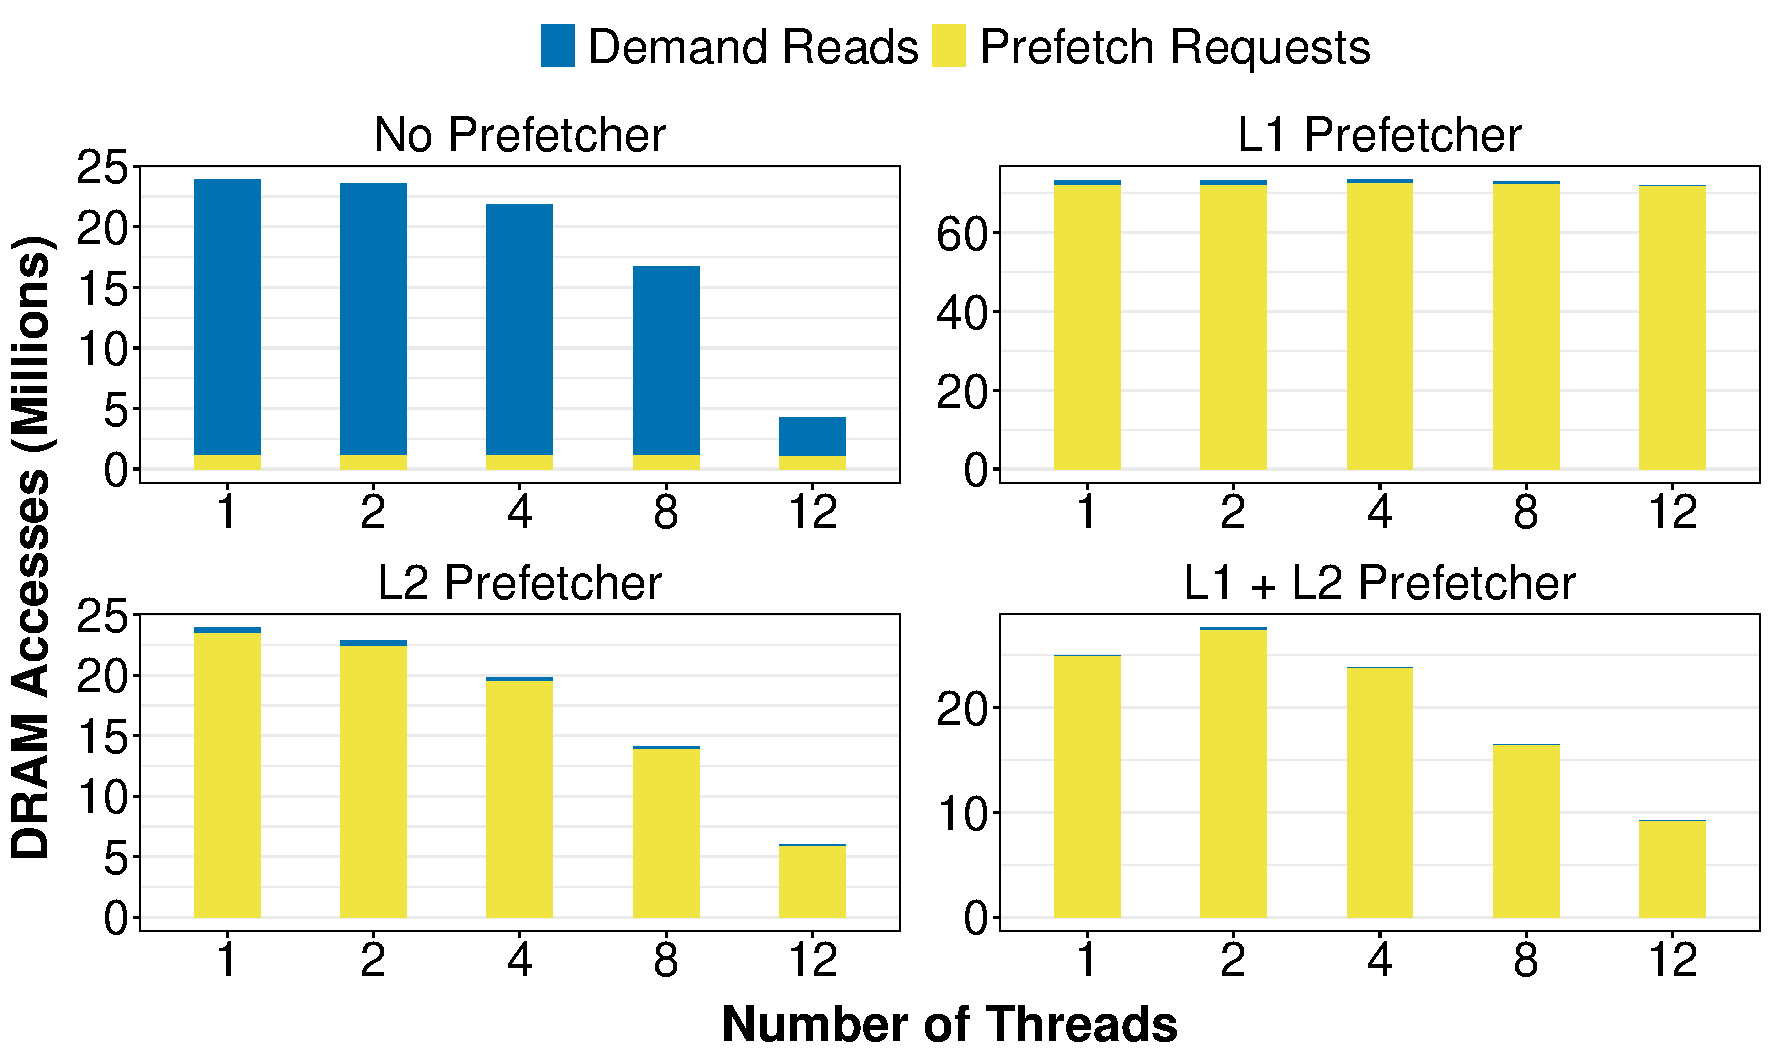
\includegraphics[width=.8\linewidth]{figures/fig4.pdf}
    %\caption{\vsg{Number of Last Level Cache (LLC) read misses for the CG application, with each prefetching algorithm and varying the number of threads (log scale on $y$ axis), input class A.}}
    \caption{CG main memory accesses, originated by demand reads and prefetches requests, for input class A.}
    \label{fig:drampapi}
\end{figure}


%This effect is less likely to happen in applications with regular memory accesses, where the memory addresses required by the threads are more uniformly partitioned. 
%Thus, this memory address will likely already be in the LLC (which is shared among cores in Skylake), making it easier to be accessed from the L2 and L1 caches -- and easier to be prefetched as well -- by the other cores. % In this regard, a large cache sizes, notably the LLC and L2 will help in magnifying this effect.

%However, we observe that the same behavior does not occur in the executions with the L2 prefetcher and the L1+L2 prefetchers.
%In fact, the number of DRAM accesses increases as we increase parallelism \textbf{check this once we have the plots}, meaning that somehow the working set is not fitting so well within the cache memory anymore.
%To understand this behavior, we need to look more closely at the thread communication in CG.
%Generally speaking, communication between threads occurs through shared memory, with threads writing and reading in shared addresses.
%However, to keep the data coherency in the several levels of the memory hierarchy, the action of writing into a memory address causes the cache coherence protocol to change the line state to MODIFIED and to invalidate all other copies of the data in the memory.
%Therefore, when a thread requests an address that is found as MODIFIED in the LLC or in another core's private cache levels, the thread is probably reading from an address used for communication with another thread.

% \ms{sugestao comentar}
% Although the working set increasingly fits in the cache hierarchy as we use more cores, we have observed that the total number of L2 cache misses does not decrease for larger number of threads.
% Since CG is communication intensive (see Figure~\ref{fig:figcomma}), this means that each thread requires significant work from the cache coherence protocol, since reading data written by another thread causes the cache coherence protocol to change the line state to MODIFIED and to invalidate all other copies of the data in the memory.
% Therefore, in Figure~\ref{fig:HITM_CG}, we show the number of load instructions from all cores whose requested data hits the LLC in the MODIFIED state, while varying the number of threads and available prefetchers, for the input class A.
% The amount of communication is similar for all prefetcher configurations, and closely follows the application's IPC for the configurations without the L2 prefetcher.\ms{tb n entendi} \textcolor{red}{\textbf{Não entendi direito :-(}}
% This increase on the LLC hits is also linked to the decrease of DRAM accesses, as a larger part of the working set of the application is now present in the cache.
%\fbm{recoloquei as linhas acima pois sao mt relevantes mesmo so com a figura de DRAM}

%We can see that without the prefetcher's action, the number of requested cache lines found in the LLC on the MODIFIED state is more prominent than when both prefetchers L1 and L2 are enabled.
%Once the amount of communication made by the application is the same regardless of the prefetching mechanism, the smaller number of hits to data in the MODIFIED state indicates that some of this data is not even being found in the cache.
%This indicates that the wrong predictions performed by the L1+L2 prefetchers and by the L2 prefetcher are causing the eviction of part of the useful data from the cache.
%Therefore, in CG we observe that the performance loss of these executions results from the already mentioned contention that arises with parallelism, but also from the prefetcher-related cache pollution.
%Moreover, the L2 prefetcher is the most responsible prefetcher for the contention in shared resources since its prefetch requests are the ones that reach the off-core shared resources, as the LLC and the mesh interconnection among cores.

% \begin{figure}[!htb]
%     \centering
%     
\includegraphics[width=\linewidth]{figures/legend.pdf}
%     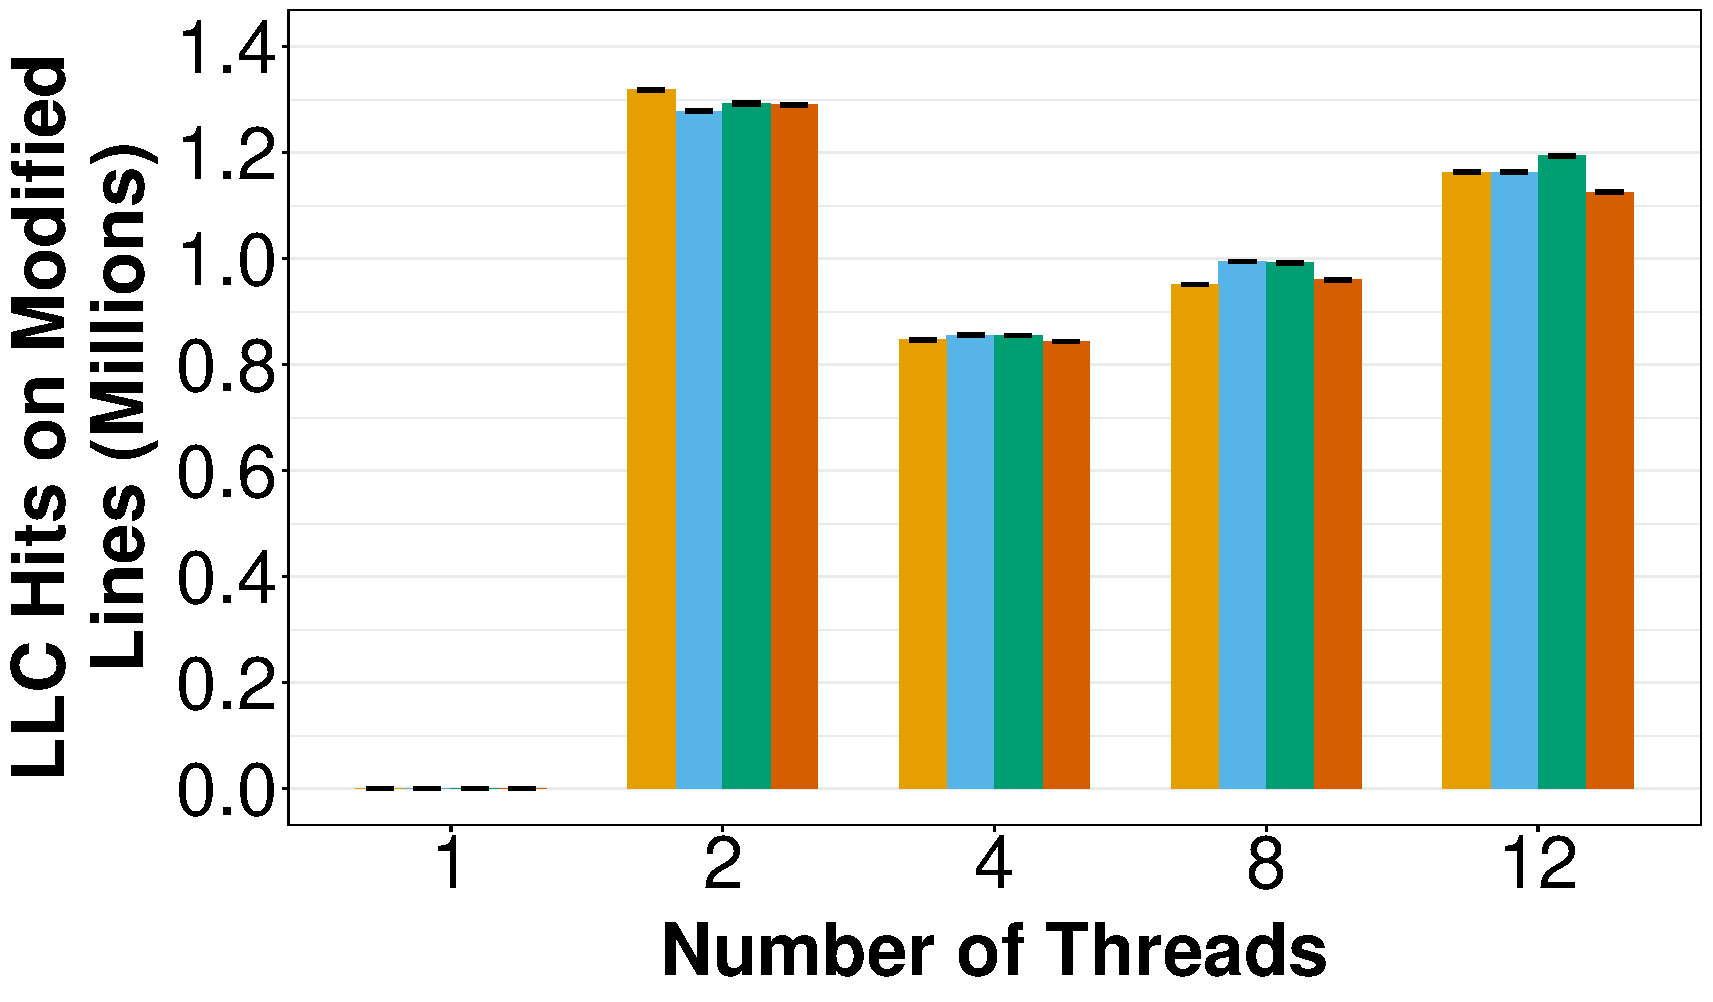
\includegraphics[width=.5\linewidth]{figures/fig5.pdf}
%   \caption{Number of HITM for each execution of the CG application, with varying number of threads, for the input class A.}
%     \label{fig:HITM_CG}
% \end{figure}

% só L1 e sem pref -> aumenta o IPC
% 

In Figure~\ref{fig:ipc}, we also notice a contrast in the performance of configurations with the L2 prefetcher, and those without.
Configurations with the L2 prefetcher do not have an IPC increase with a higher number of cores, as the L2 prefetcher is correctly speculating and bringing the data to the caches even with a low core count and low amount of cache.
On one hand, the IPC tendency of configurations with an L2 prefetcher is to decrease, as the prefetcher effectively hides the latency of DRAM accesses, but increasing the number of cores generates contention in the DRAM access.
On the other hand, configurations without the L2 prefetcher cannot hide this latency, and their IPC increase as the application is able to retain larger portions of the working set in higher quantities of private non-inclusive L2 caches.


%\ms{talvez tirar essa parte}
%Therefore, to summarize the CG case, we conclude that, due to the large amount of communication, a thread may request a memory address that had already been brought into closer cache levels by other threads. \ms{e qual a consequencia disso?} \ms{e por isso tal coisa acontece com o prefetch} \ms{qual a consequencia disso para a explicacao do comportamento do sem prefetch e do L1 Prefetch}
%When we increase parallelism, more threads repeat this behavior, and the application has more cache space available due to the addition of more than 1 MB of non-inclusive cache for each core being used.
%Therefore, the executions without prefetcher and with only the L1 prefetcher are able to take \textcolor{red}{\textbf{\sout{huge}}} leverage of the bigger cache space, surpassing the effect of the contention that arises with parallelism.
%(iii) however, when the L2 prefetcher is enabled, the application suffers from intensive prefetch-related cache pollution, which disguises the benefits of more cache space and harms the application performance;
%(iv) therefore, the performance gains observed for the executions without the L2 prefetcher are the result of the less intensive pollution and memory contention being created, allowing the application to take leverage 




\subsection{Effects of Different Input Classes}
\label{subs:NAS_WAB}


Up to this point, we analyze the relationship between the prefetcher and the parallelism increase with fixed input size.
However, the memory requirements of different HPC applications may vary substantially, requiring different execution parameters. 
For instance, when considering small input sizes, an execution with several threads may highlight communication effects, which will play a decisive role in the application's performance.
Simultaneously, the prefetcher's effectiveness may also be disturbed if we increase the parallelism in communication-intensive applications.
In this section, we aim to better understand how the prefetcher influences performance when we vary the application's memory requirements. %\fbm{again, we don't even explain the prefetcher's functionality details, so "behave" is not a great word choice imho}

In Figure~\ref{fig:nas_wab}, we present the IPC results for the SP application with different thread counts, different hardware prefetcher configurations, and variable input sizes, using NPB classes W, A, and B.
We present the results only for the SP application since the same behavior is observed for all other NPB applications.
The first point to be noted is that as we increase the problem size, the prefetcher's influence on the application's performance increases as well. 
If no prefetcher is enabled, class W suffers from a modest performance loss, while classes A and B are able to improve their performance by up to two times with all prefetchers activated.
Since class W has smaller memory requirements, any prefetcher that can predict a simple access pattern may already be able to fetch a significant part of the application's working set in advance.
Therefore, the performance decrease observed as we increase parallelism in class W is caused by the thread communication overhead observed over small input sizes, which can not be entirely solved by the prefetcher.
%not caused by long-latency accesses or by memory contention, but by thread communication itself, which can not be entirely solved by the prefetcher.


When we compare the performance reduction observed with the increase of parallelism for classes A and B, we identify that a bigger problem size suffers from a more dramatic loss.
As we increase the parallelism of the execution with the class A, the execution without prefetcher does not suffer performance reduction.
For class B, however, a small performance loss is observed even with all hardware prefetchers disabled.
This points out that the source of performance loss for class A is strictly related to the previously noted contention that arises with the prefetcher action in a multicore system.
For class A, the working set appears to fit entirely within the on-core memory levels; consequently, the application only demonstrates performance loss when facing prefetcher-related contention.
However, as the problem size scales, more off-core long-latency memory accesses are necessary since the working set does not fit entirely inside the on-core memory levels.
For this reason, these long-latency memory accesses, together with the prefetcher-related memory contention, harm the application's performance more fiercely in class B.


\begin{figure}
    \centering
    %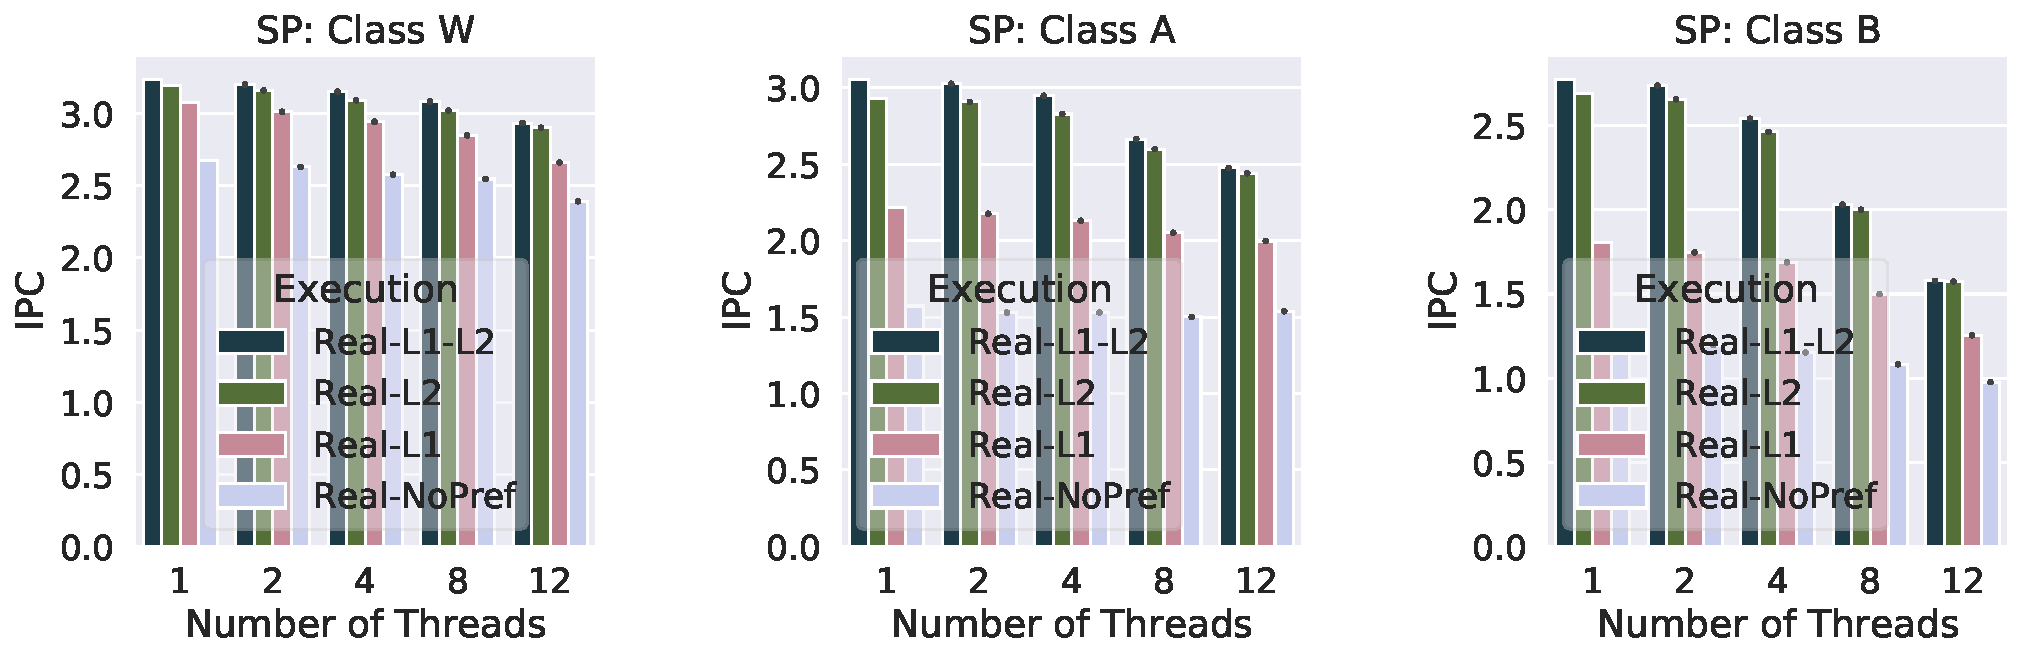
\includegraphics[width=.8\linewidth]{figures/IPC_sp_all_allclass_cei.pdf}
    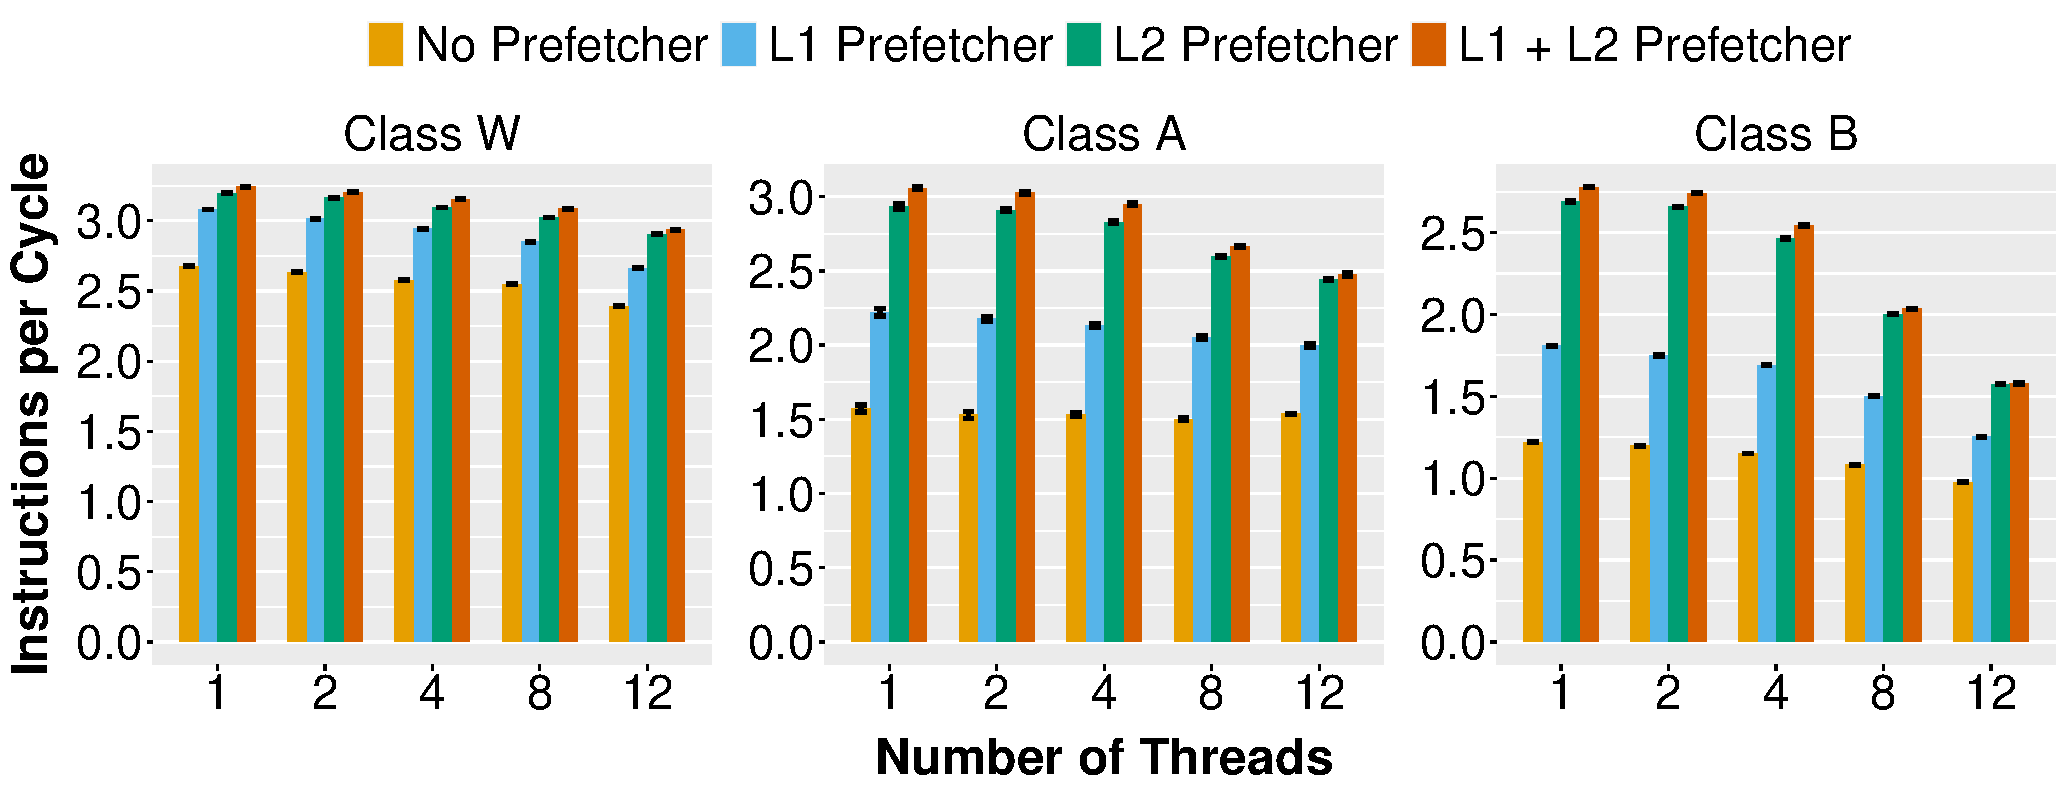
\includegraphics[width=\linewidth]{figures/fig6.pdf}
    \caption{IPC results of the NPB SP application, using input classes W, A, and B.}
    \label{fig:nas_wab}
\end{figure}




\begin{comment}

\subsubsection{Turbo Boost Impact}
\label{subs:turbo}

\vsg{aparentemente nada disso aqui faz sentido e da pra tirar a secao inteira :) }


As already mentioned, all the previous results were collected from executions with the Intel Turbo Boost~\cite{rotem2012turbo} disabled in order to increase experimental control.
The Turbo Boost technology automatically and dynamically allows processor cores to run at a higher frequency to maximize the performance while respecting the Thermal Design Power (TDP) definition.
The decisions made by the Package Control Unit (PCU), the brain behind the power-management engine, take into account several different hardware and software constraints:
i) voltage, frequency and power capabilities;
ii) power-delivery capabilities;
iii) die temperature;
iv) the operational system explicit control;
v) workload and usage characteristics.
Consequently, Turbo Boost can present varying contributions depending on the context of execution and on the application's behavior.
For instance, CPU-bound applications can easily take leverage of the higher frequency delivered by the Turbo Boost action, while memory-bound applications may display negligible gains~\cite{lo2014turbo,marques2019turbo}.
Therefore, in this section, we seek to understand how Turbo Boost affects the parallel applications as we increase the number of threads for each of the available prefetchers.


\fbm{reescrever pq figuras foram feitas de jeito diferente}
In Figures~\ref{fig:noturbo} and ~\ref{fig:turbo}, we compare the IPC of the \textbf{XXX} application with Turbo Boost enabled to the execution with Turbo Boost disabled, while varying the number of threads and the prefetchers being used, with the input class A.
The first observation is the most substantial performance variation among cores with the action of Turbo Boost, which is a direct result of how the aforementioned parameters may interfere in the runtime decision made by the power-management algorithms.
I really need the plots to talk more about all this :/

%\begin{figure}[b]
%    \centering
%    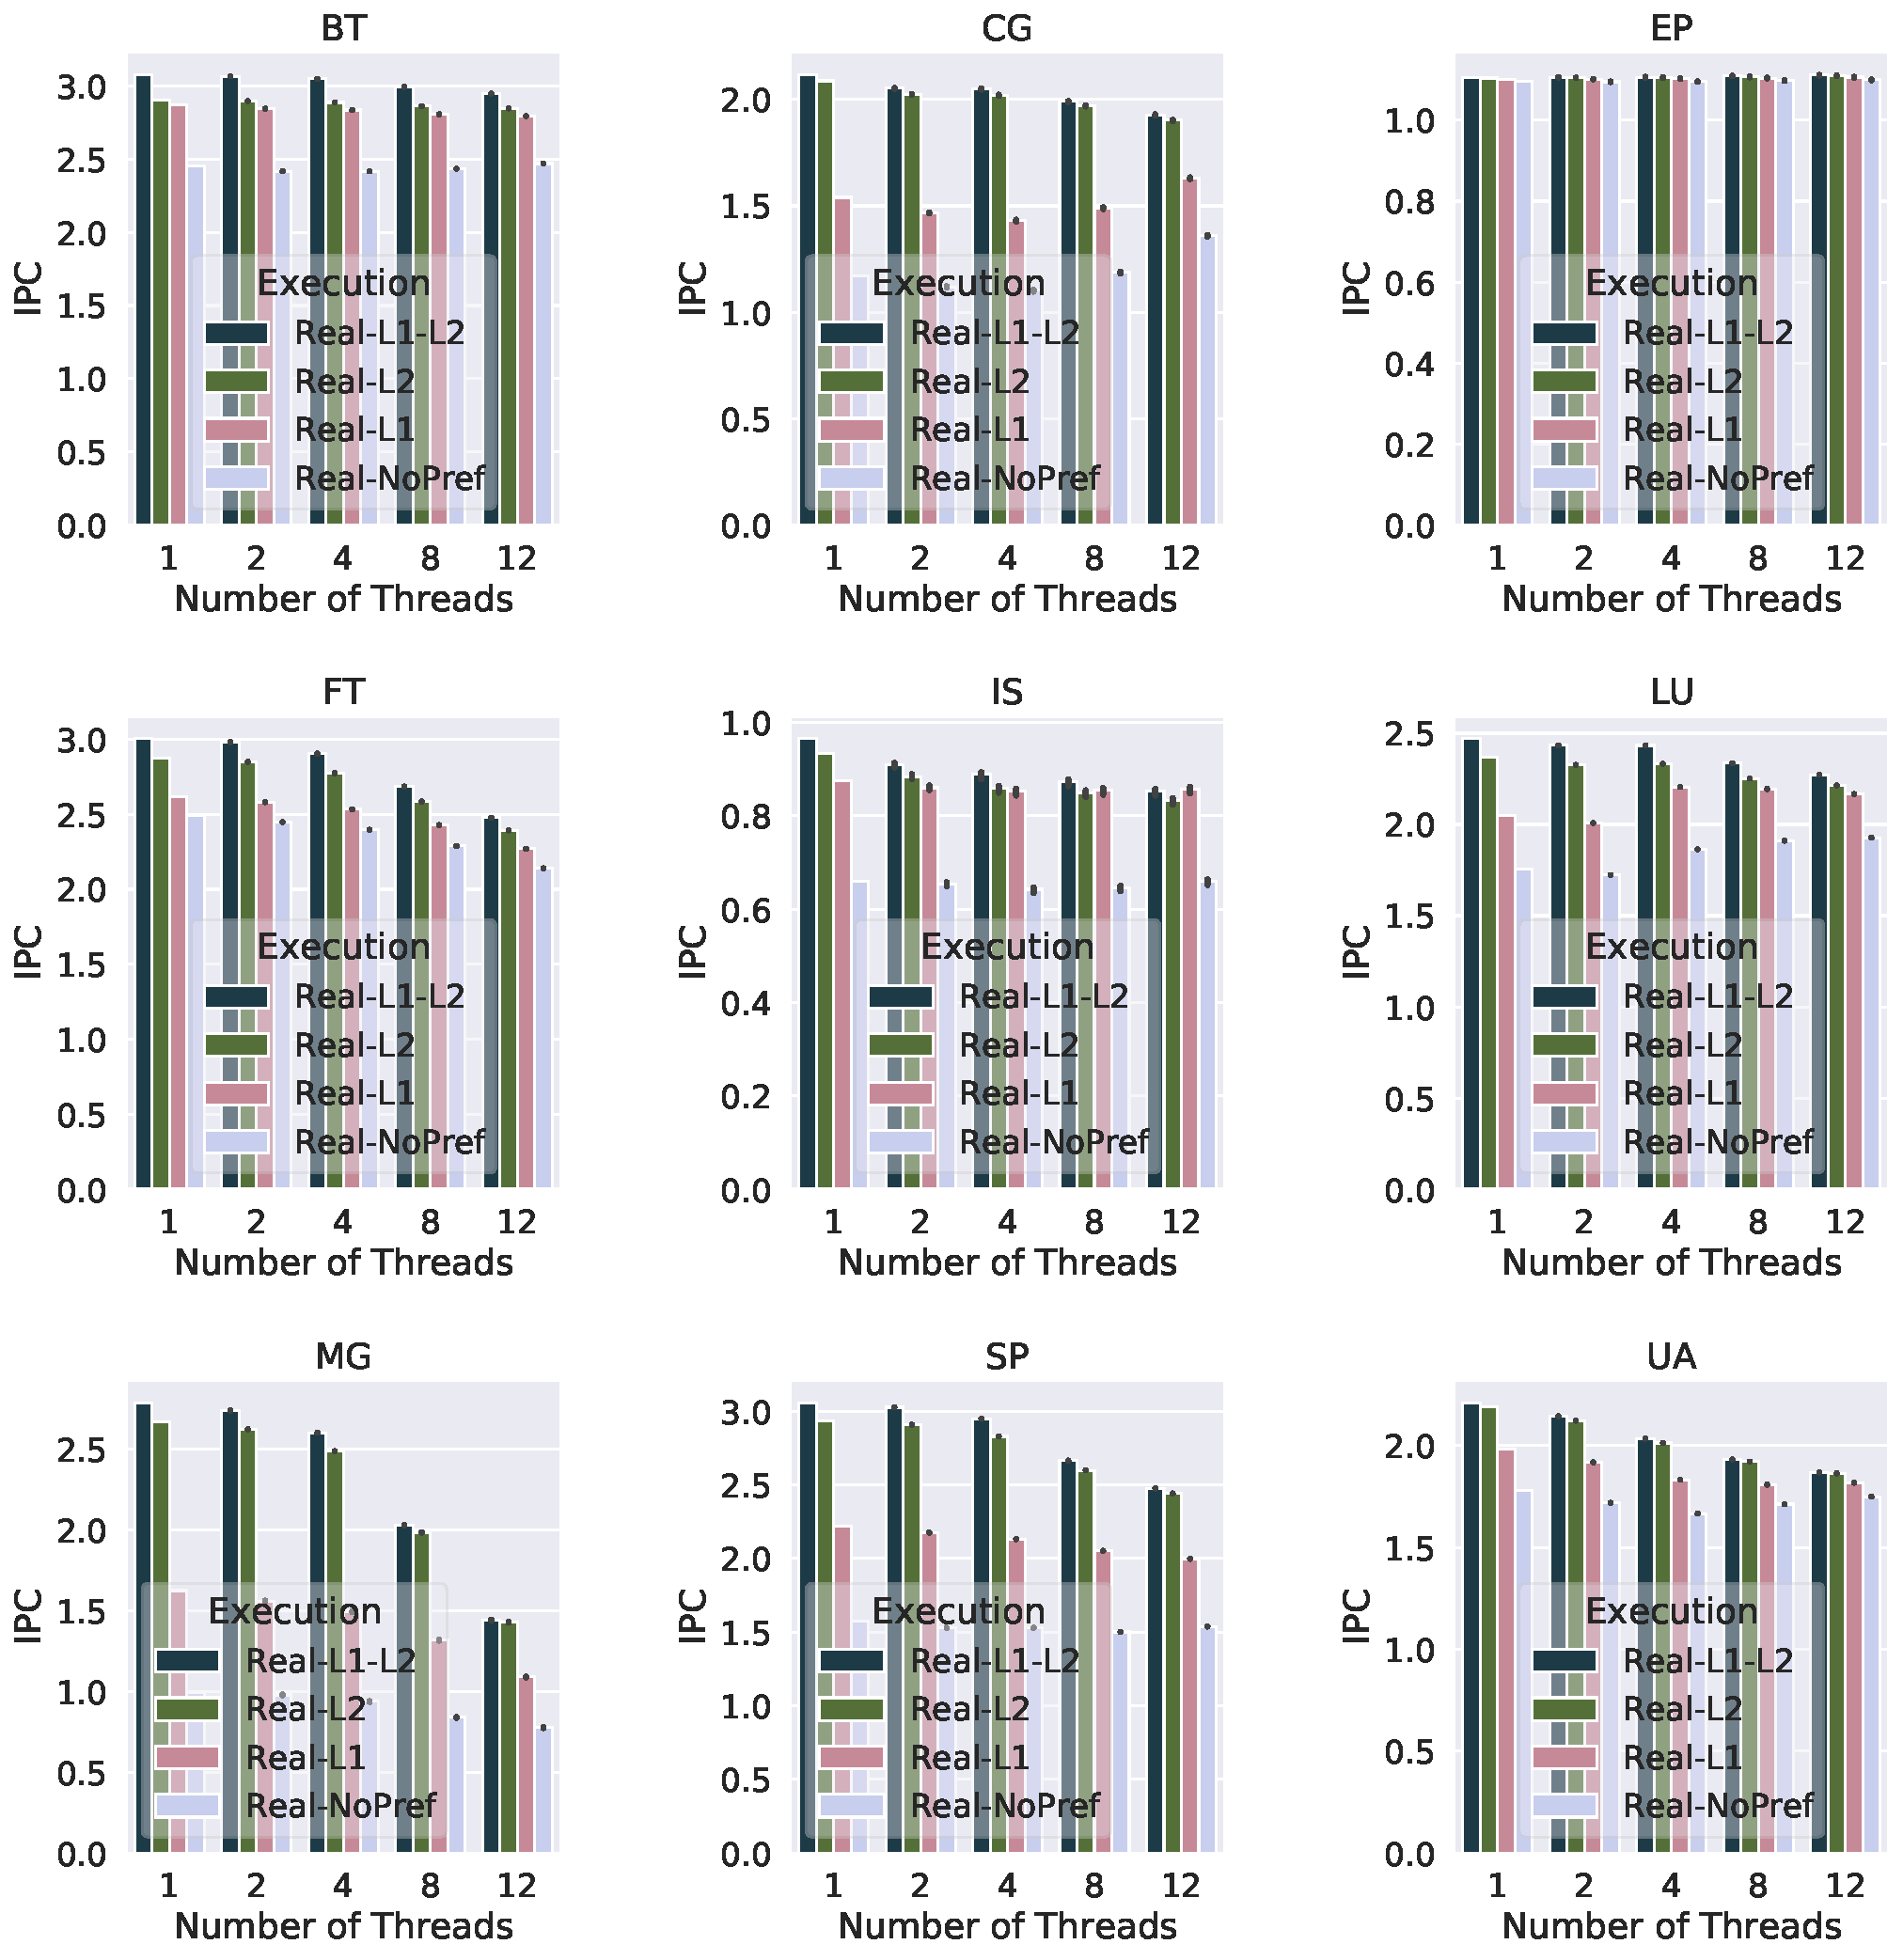
\includegraphics[width=.8\linewidth]{figures/IPC_A_all_subm2_cei_noturbo.pdf}
%    \caption{IPC metric for all benchmarks with Turbo Boost disabled.}
%    \label{fig:noturbo}
%\end{figure}

%\begin{figure}[b]
%    \centering
%    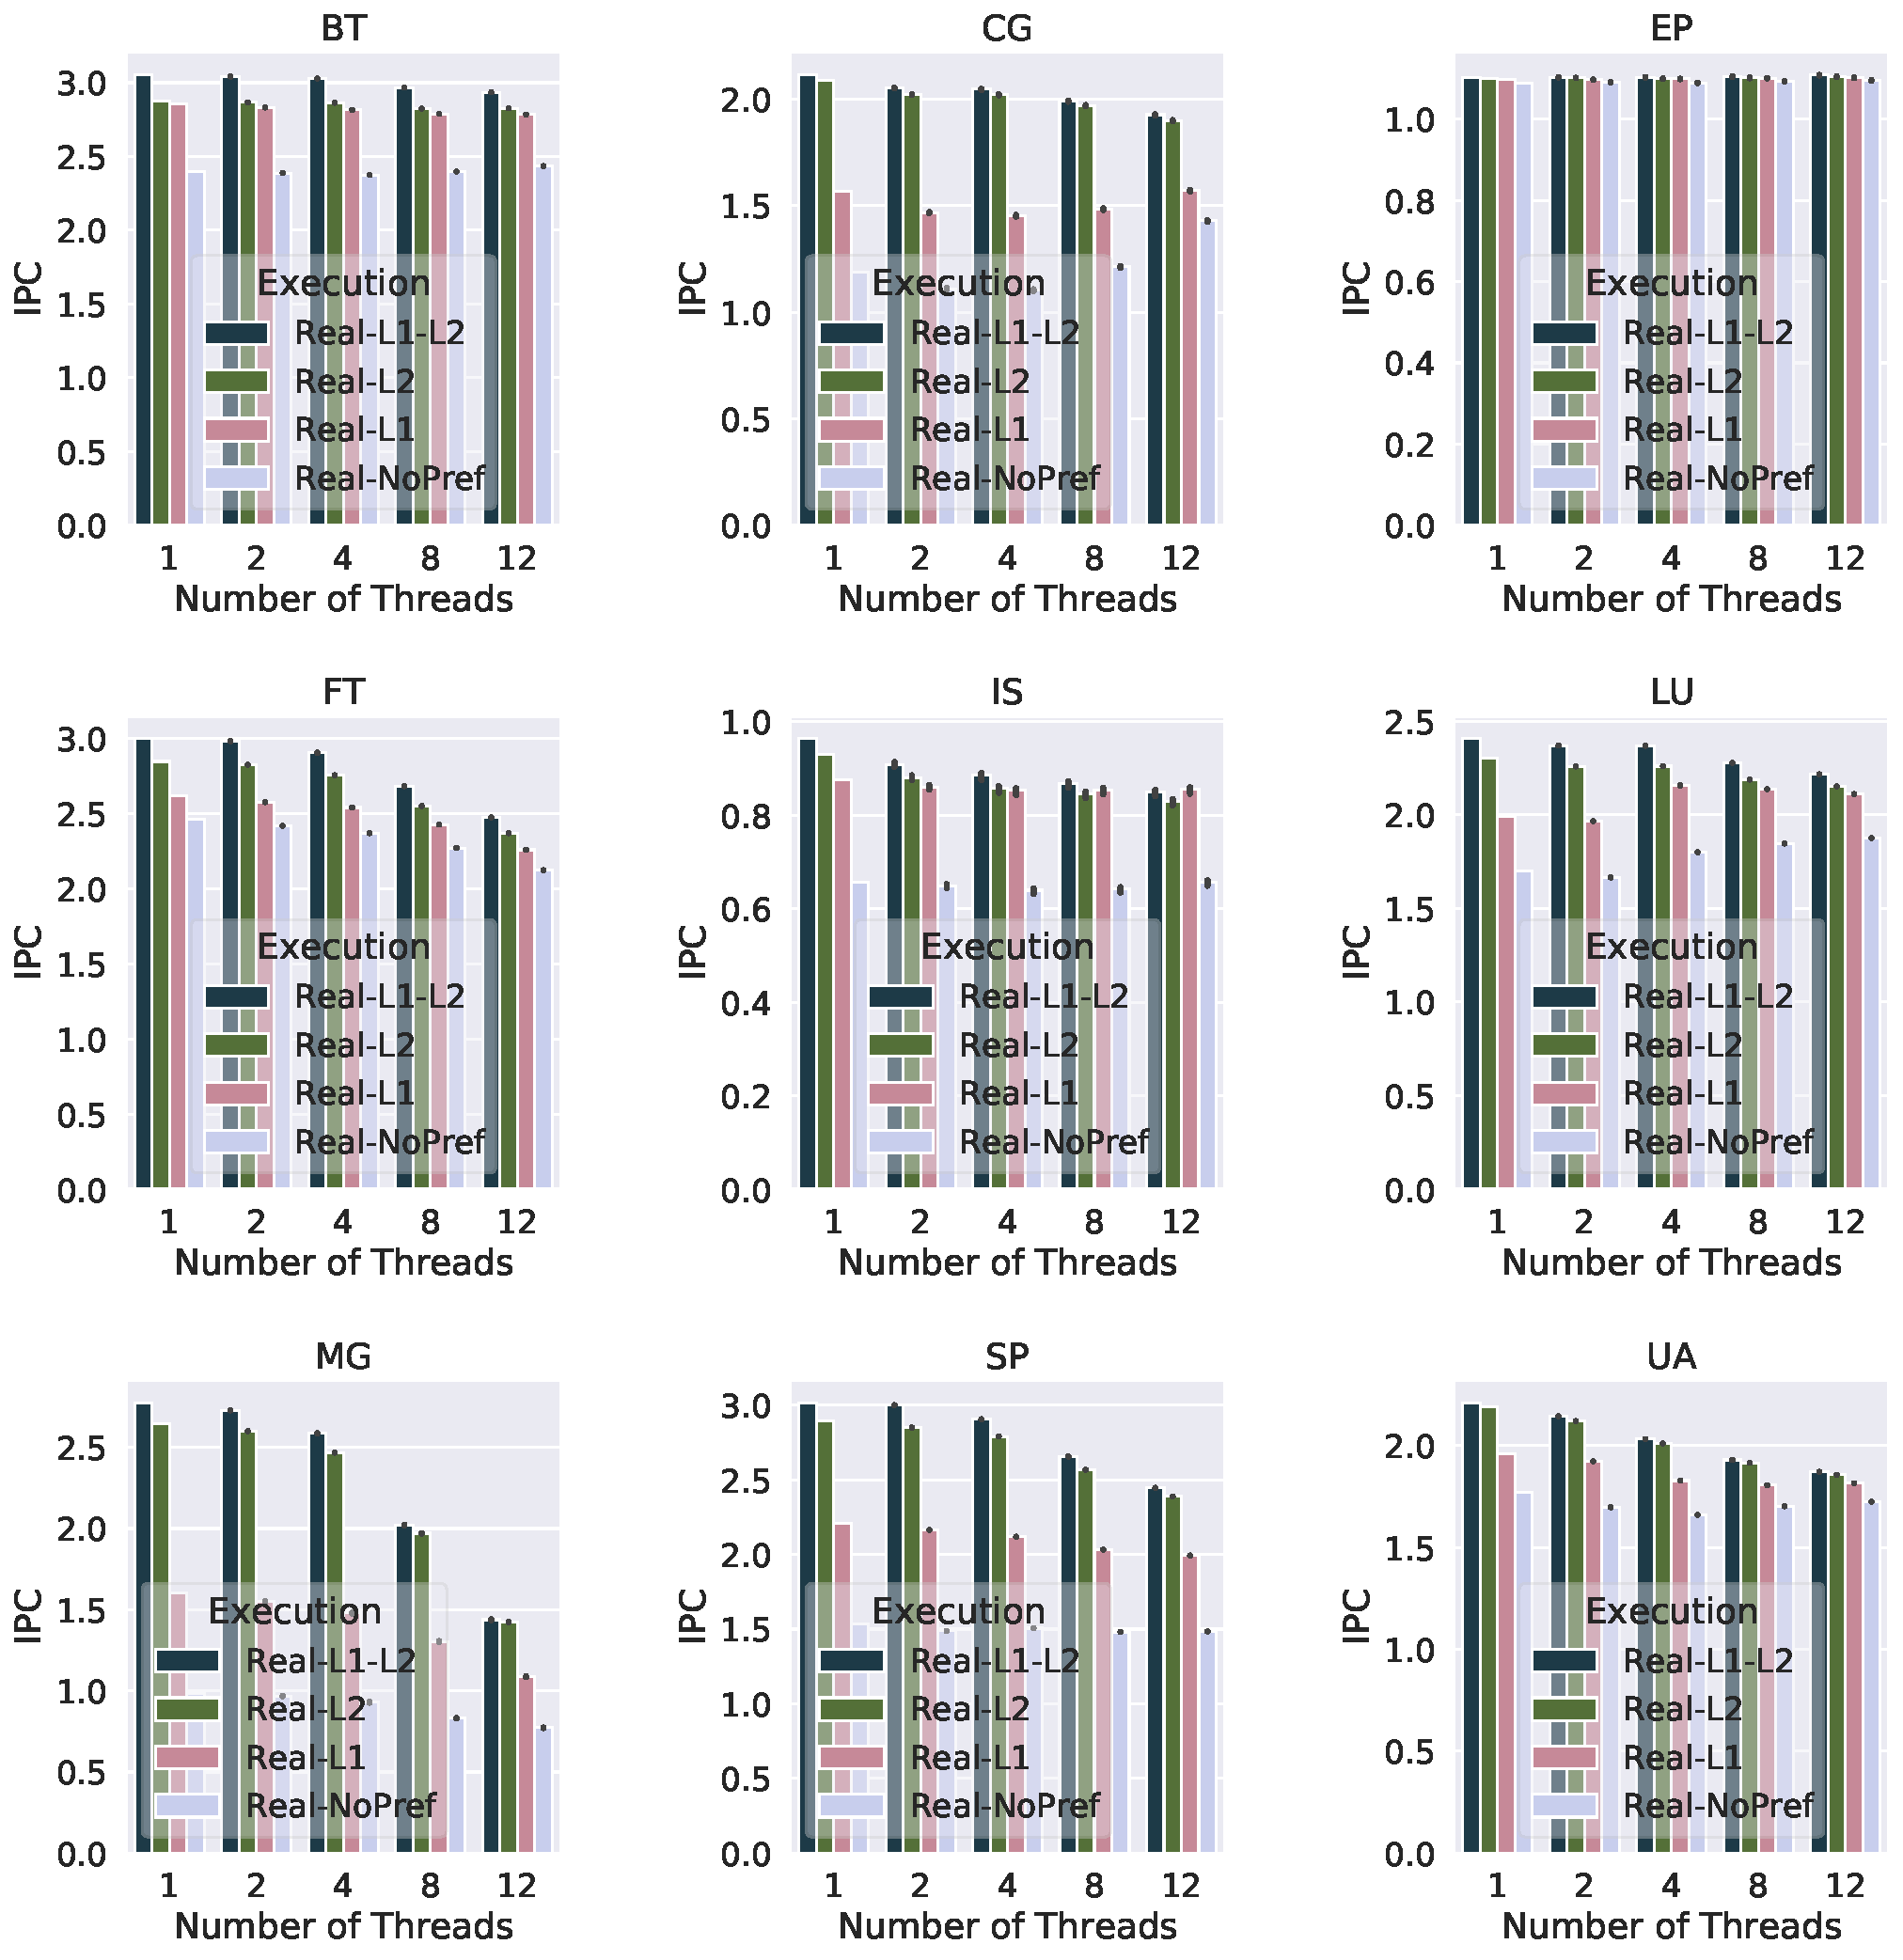
\includegraphics[width=.8\linewidth]{figures/IPC_A_all_subm2_cei_turbo.pdf}
%    \caption{IPC metric for all benchmarks with Turbo Boost enabled.}
%    \label{fig:turbo}
%\end{figure}


com relação ao turbo boost:
- o que concluímos so far: turbo boost parece ser meio ruim, reduz o IPC. Aumentando a freq do clock, as insts terminam mais rápido, porém a freq do bus/memória continua a mesma, então leva mais ciclos pra completar uma instrução pq a instrução terminou rápido e ficou esperando por dado. Dessa forma, o IPC cai com turbo boost ativado. Apps com muita comm ou memory bound sofrem mais. 
- temos: execs com PAPI com tubo desativado e ativado, gráfico da exec sem turbo boost
- precisamos: gráficos com turbo boost (e papi) pra mostrar a perda de desempenho
- notamos também que com turbo boost, a degradação de desempenho é maior em função no grau de paralelismo, o que pode indicar que turbo boost também não é adequado para execuções com alto grau de paralelismo, mas para confirmar isso, teríamos que executar de novo, com o PAPI e turbo boost. Não temos tempo pra isso

\end{comment}



\begin{figure}[b]
    \centering
    %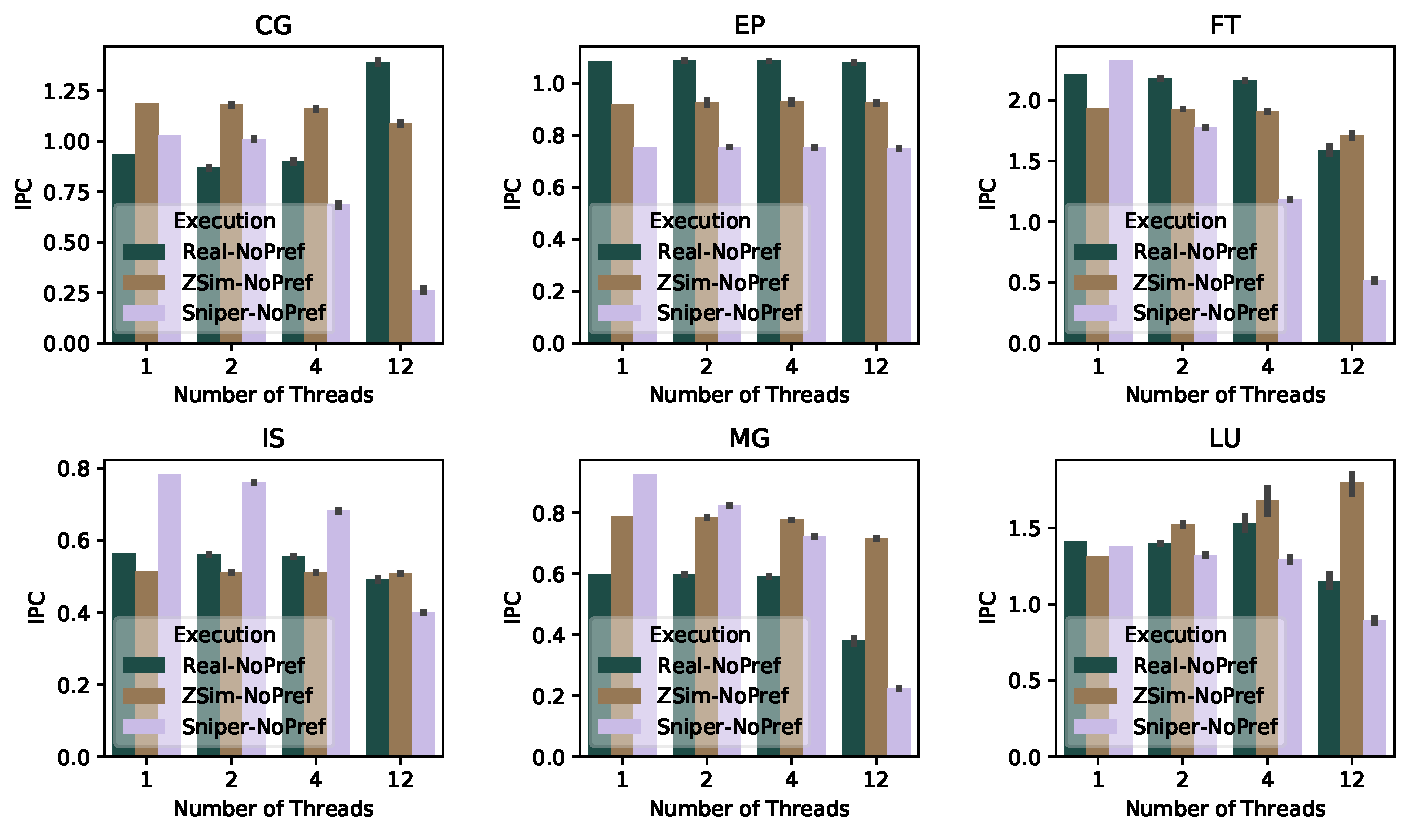
\includegraphics[width=.8\linewidth]{figures/sim_nopref_ipc.pdf}
    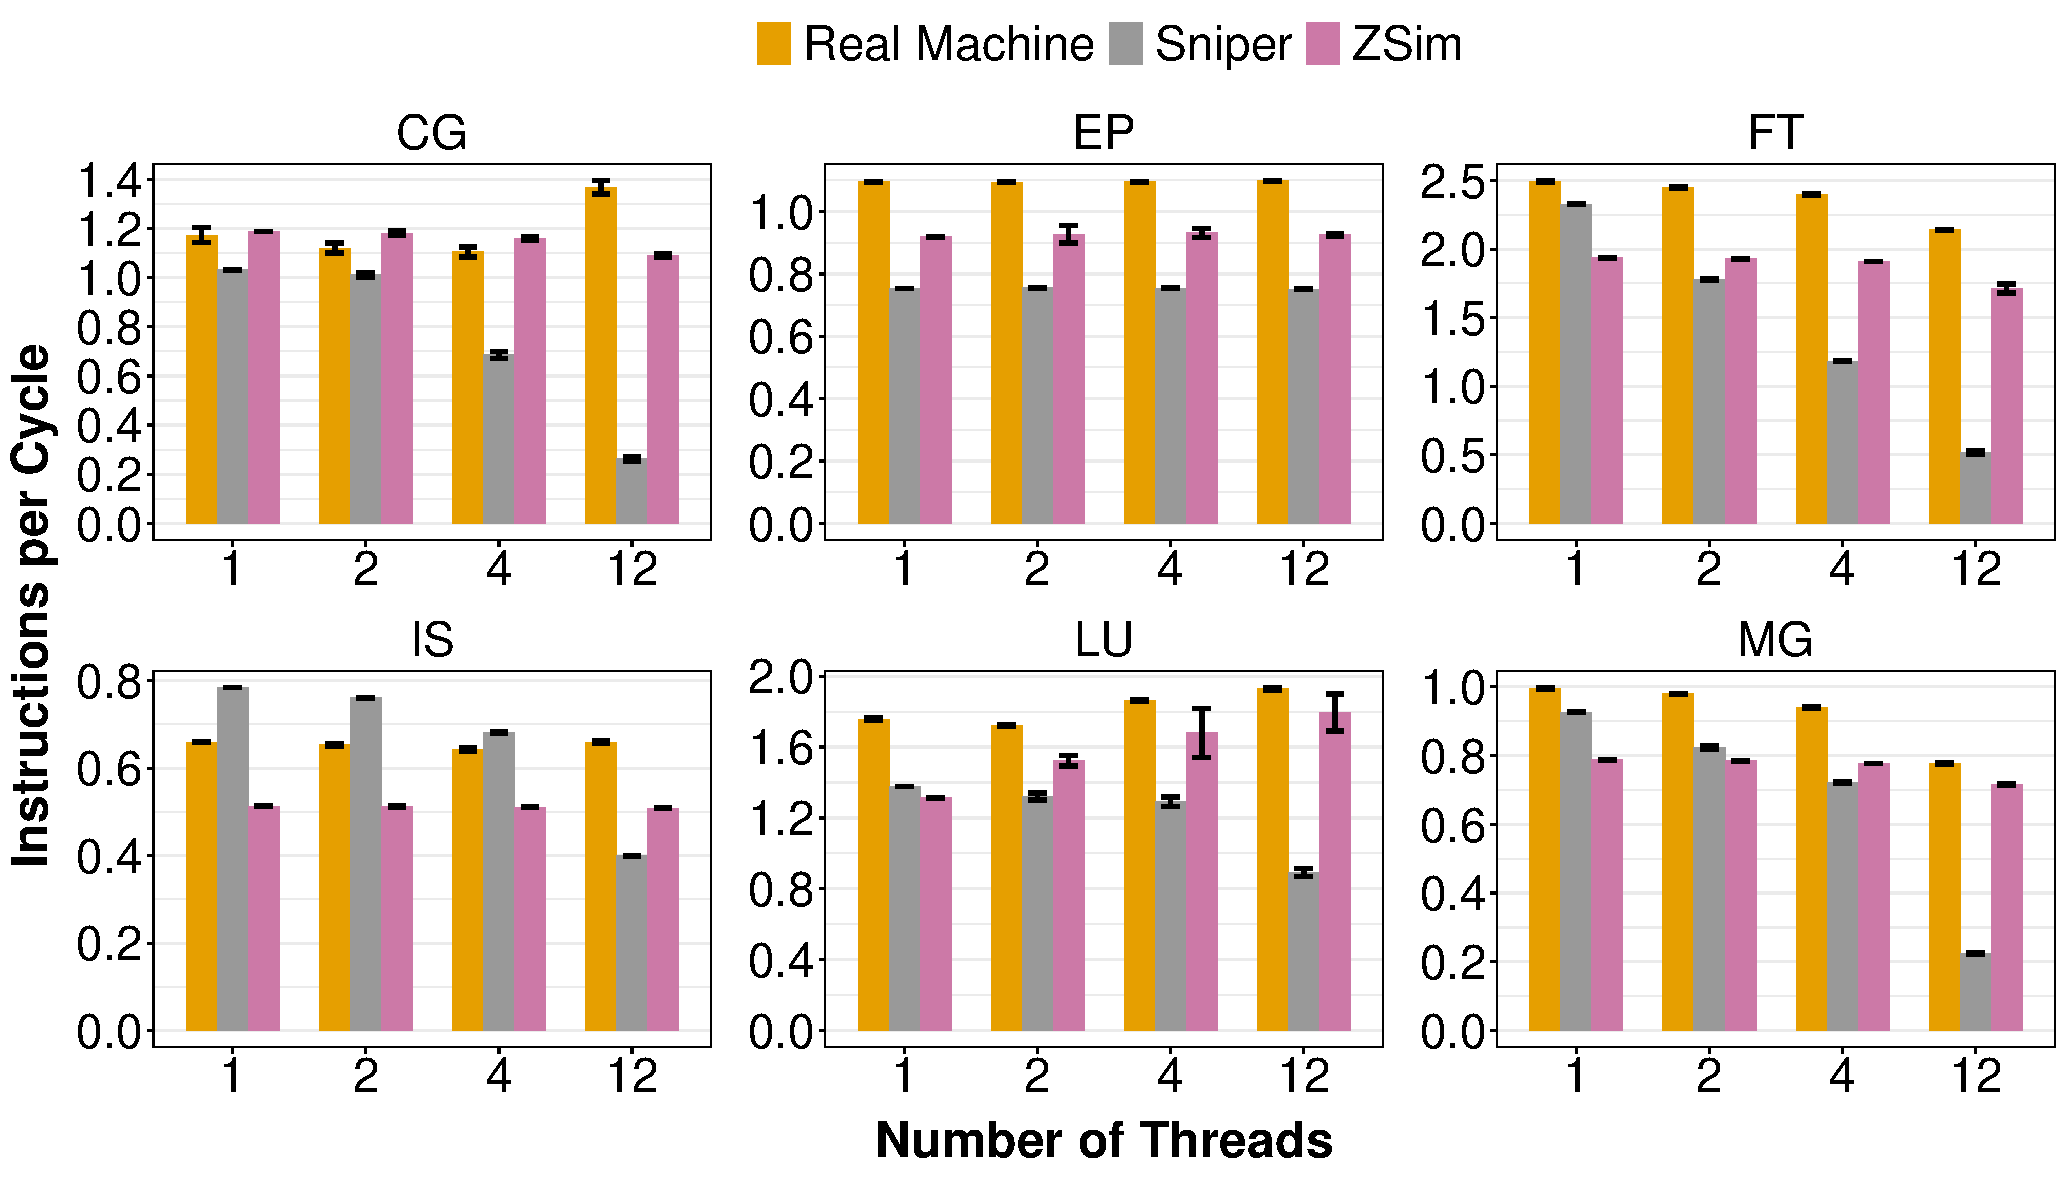
\includegraphics[width=\linewidth]{figures/fig8.pdf}
    \caption{Experimental results comparing the performance of simulation and real execution without prefetcher.}
    \label{fig:sims_nopref}
\end{figure}


%\subsection{Simulation Results}\label{subs:simulation}
%dcs: troqui para verbo (investigating) ao invés de susbstantivo (investigation)
\section{Investigating Prefetchers on Simulation}\label{sec:simulation}

As discussed in Section~\ref{sec:introduction}, parallel architecture simulation tools are necessary to develop and evaluate new techniques such as new prefetcher algorithms. In this regard, a key requirement is that these simulation tools can effectively simulate the parallel architecture and the parallel applications, bringing similar values of the metrics when compared to the real execution. In this section we therefore aim to clarify the following question: \textit{Using the ZSim and Sniper simulators, how do they behave and how accurately do they simulate NPB, accounting distinct prefetchers when possible?}

While simulators are a useful tool to test new architecture techniques, one drawback is the large amount of time that is often required by the simulations. For instance, the time to simulate the SP and BT applications of NPB using Sniper took more than one week. Sinuca~\cite{alves2015sinuca}, which is another parallel architecture simulator, took even more time to simulate, exceeding the maximum execution time allowed by our computing infrastructure. In this regard, we had to discard Sinuca from the study and with Sniper we simulated only a subset of the NPB applications, notably CG, EP, FT, IS, LU, and MG. 
We also only analyzed the simulation of prefetchers with the Sniper simulator, since ZSim does not simulate memory prefetchers. 
% citar o survey a respeito do tempo de simulação



\begin{figure}[b]
    \centering
    %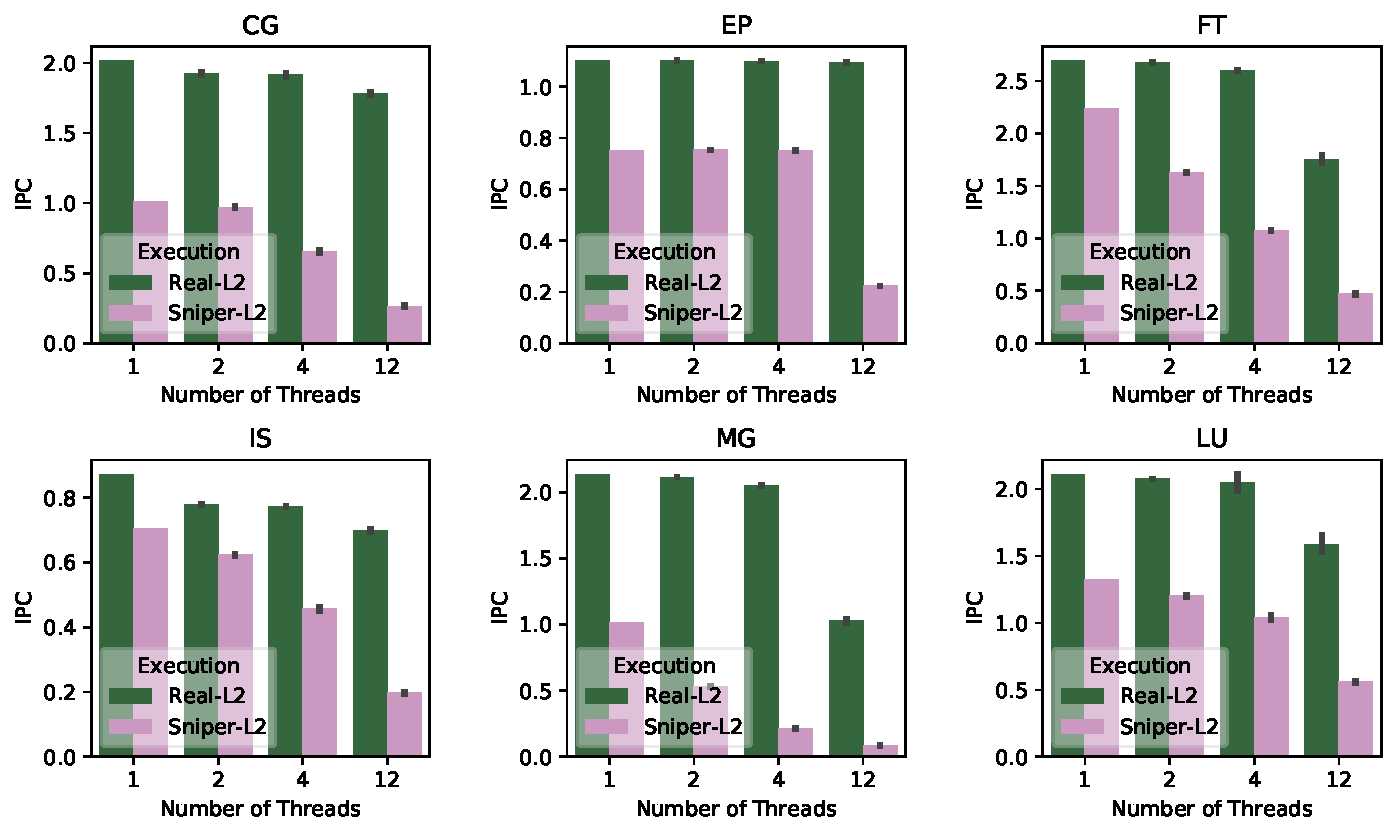
\includegraphics[width=.8\linewidth]{figures/sniper_l2_ipc.pdf}
    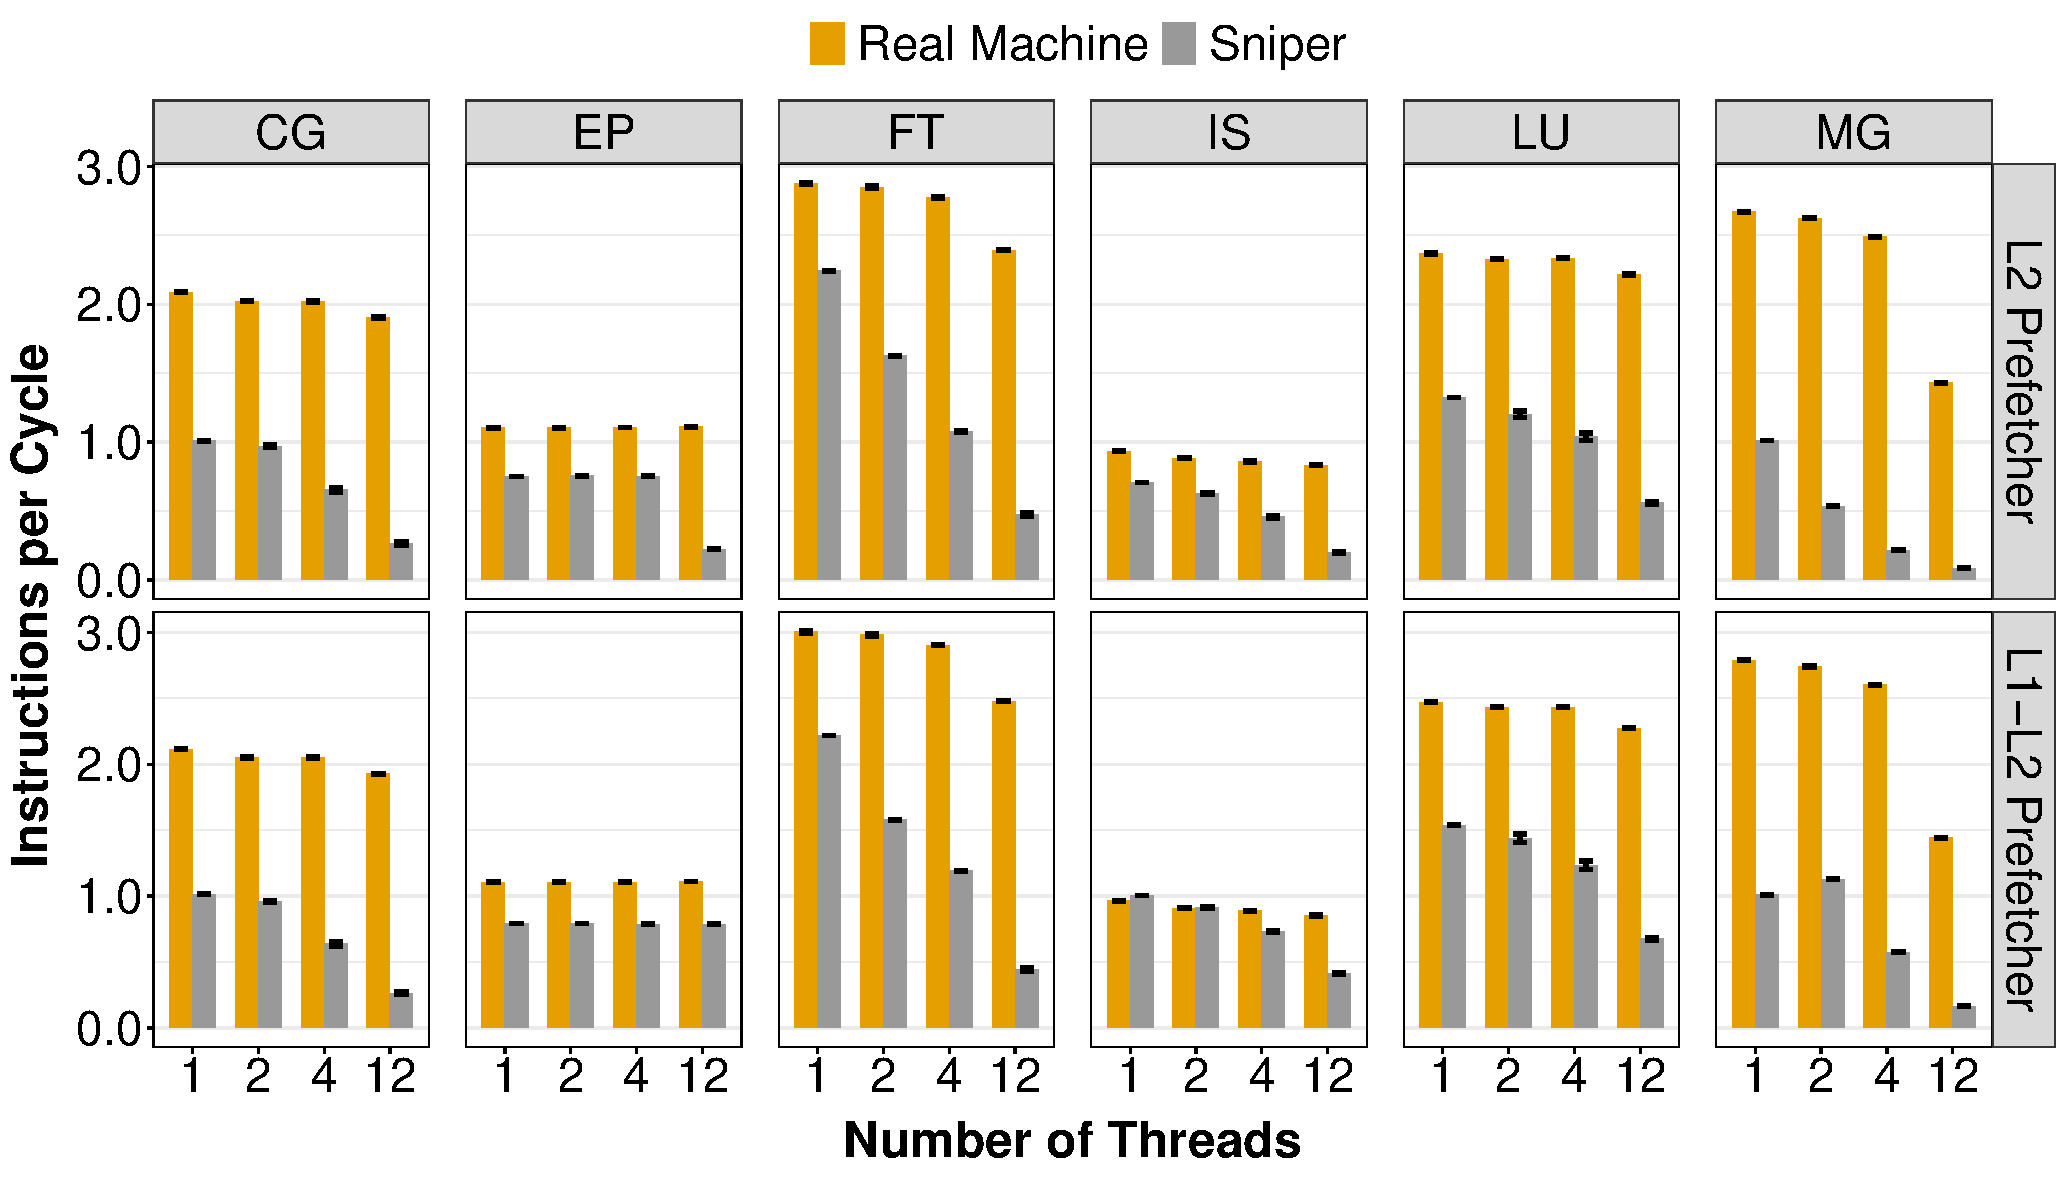
\includegraphics[width=\linewidth]{figures/fig88.pdf}
    \caption{Comparison of Sniper's L2 and L1+L2 prefetchers performance to the real executions results.}
    \label{fig:sniper_l2}
\end{figure}

Figure~\ref{fig:sims_nopref} shows the obtained IPCs when no prefetcher is used for six of the NPB applications, namely CG, EP, FT, IS, MG, and LU, simulating the input class A.
For that we disabled the prefetcher on both the real execution and the Sniper simulation. 
We did not make any specific changes to ZSim for this experiment, since ZSim does not support prefetcher simulation.
%In this experiment, we disabled the prefetchers of the real machine and the Sniper and compare to the simulation of ZSim, which does not model the prefetcher behavior.


The only application where both simulators follow the real execution performance tendency is the EP. Since EP makes very little use of communication, it results in a simulation with very little contention events. 
This makes it easier for ZSim and Sniper to simulate EP, since simulating the effects of contention is arguably one of the most complex tasks in architecture simulation because of the out of order nature of contention events~\cite{sanchez2013zsim}.
%The only application where both simulators follow the real execution performance tendency is for the EP, o que pode novamente ser explicado pelo fato de o EP não estressar tanto o subsistema de memória com comunicação.
However, for applications where communication and contention are more predominant, we can notice discrepancies between the simulation and the real execution. 
This discrepancy can be quite extreme. For instance, ZSim's MG simulation with 12 threads resulted in a average IPC 1.88 times higher than in the real execution, and Sniper's CG simulation with 12 threads resulted in an average IPC 4.6 times lower than in the real execution. 
The CG application is an interesting case because both Sniper and ZSim do not seem to accurately simulate the parallel CG execution (see Section~\ref{subs:cg}).
Both simulators predict a decrease in IPC as the number of threads increase, whereas in the real execution the trend is the opposite.
%\fbm{what's the real reason behind CG's IPC increase? My educated guess here is the additional cache makes the problem fit in the cache, which happens in real execution due to non-inclusive cache, but not in simulations due to inclusive cache}
%However, em aplicações com padrão de acesso mais irregular e comunicação entre threads mais intensa, é possível notar discrepâncias no desempenho apresentado com ambos os simuladores.
%Com relação à aplicação CG, tanto ZSim quanto Sniper não conseguem representar adequadamente o comportamento observado na execução da aplicação em uma máquina real.
%Conforme observado anteriormente, a aplicação apresenta um padrão de acessos bastante irregular, que popula os diferentes níveis de cache dos diferentes núcleos com vários dados que podem vir a ser acessados por outras threads.
%É notável, portanto, que ambos os simuladores têm dificuldades para modelar acessos irregulares à memória.




% \begin{figure}[b]
%     \centering
%     %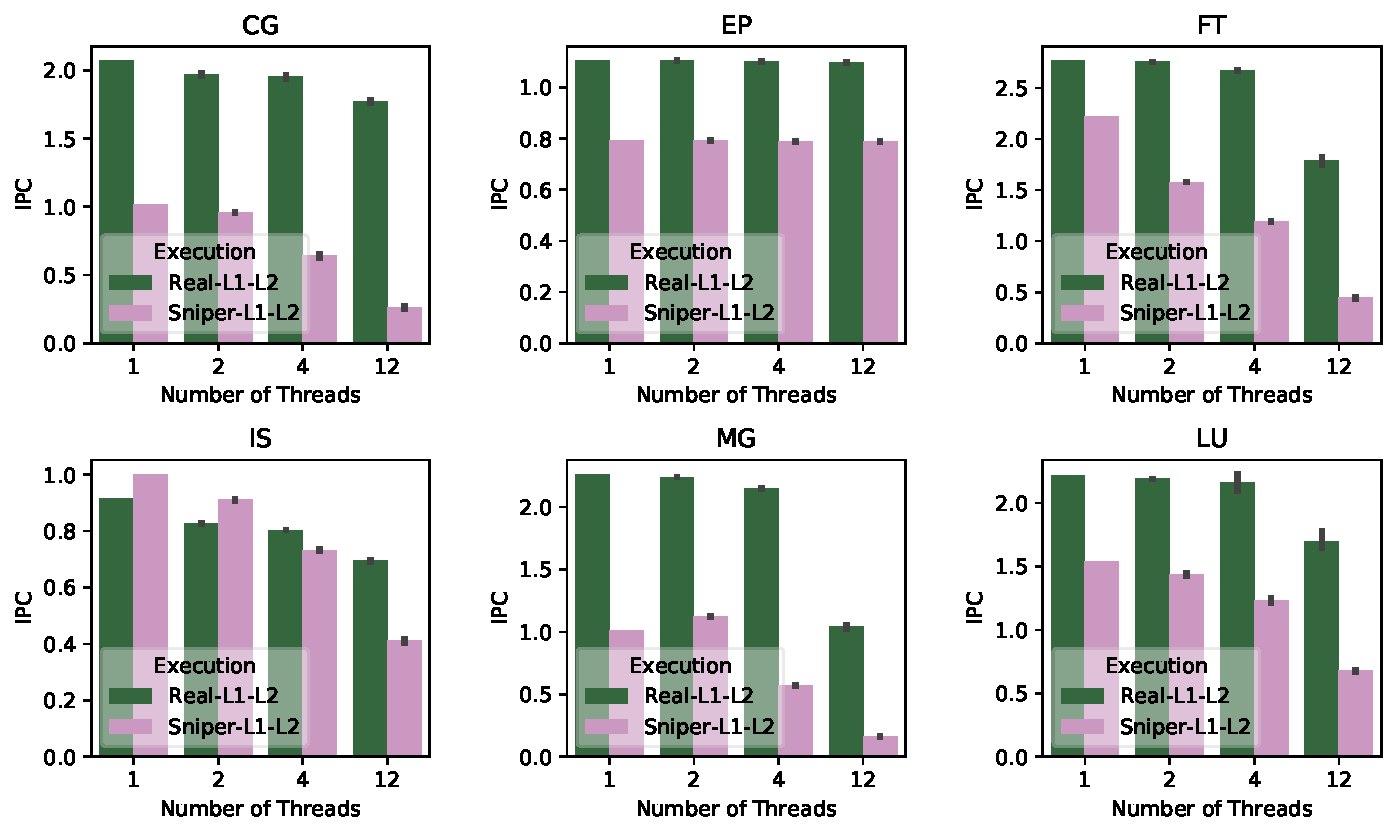
\includegraphics[width=.8\linewidth]{figures/sniper_l1_l2_ipc.pdf}
%     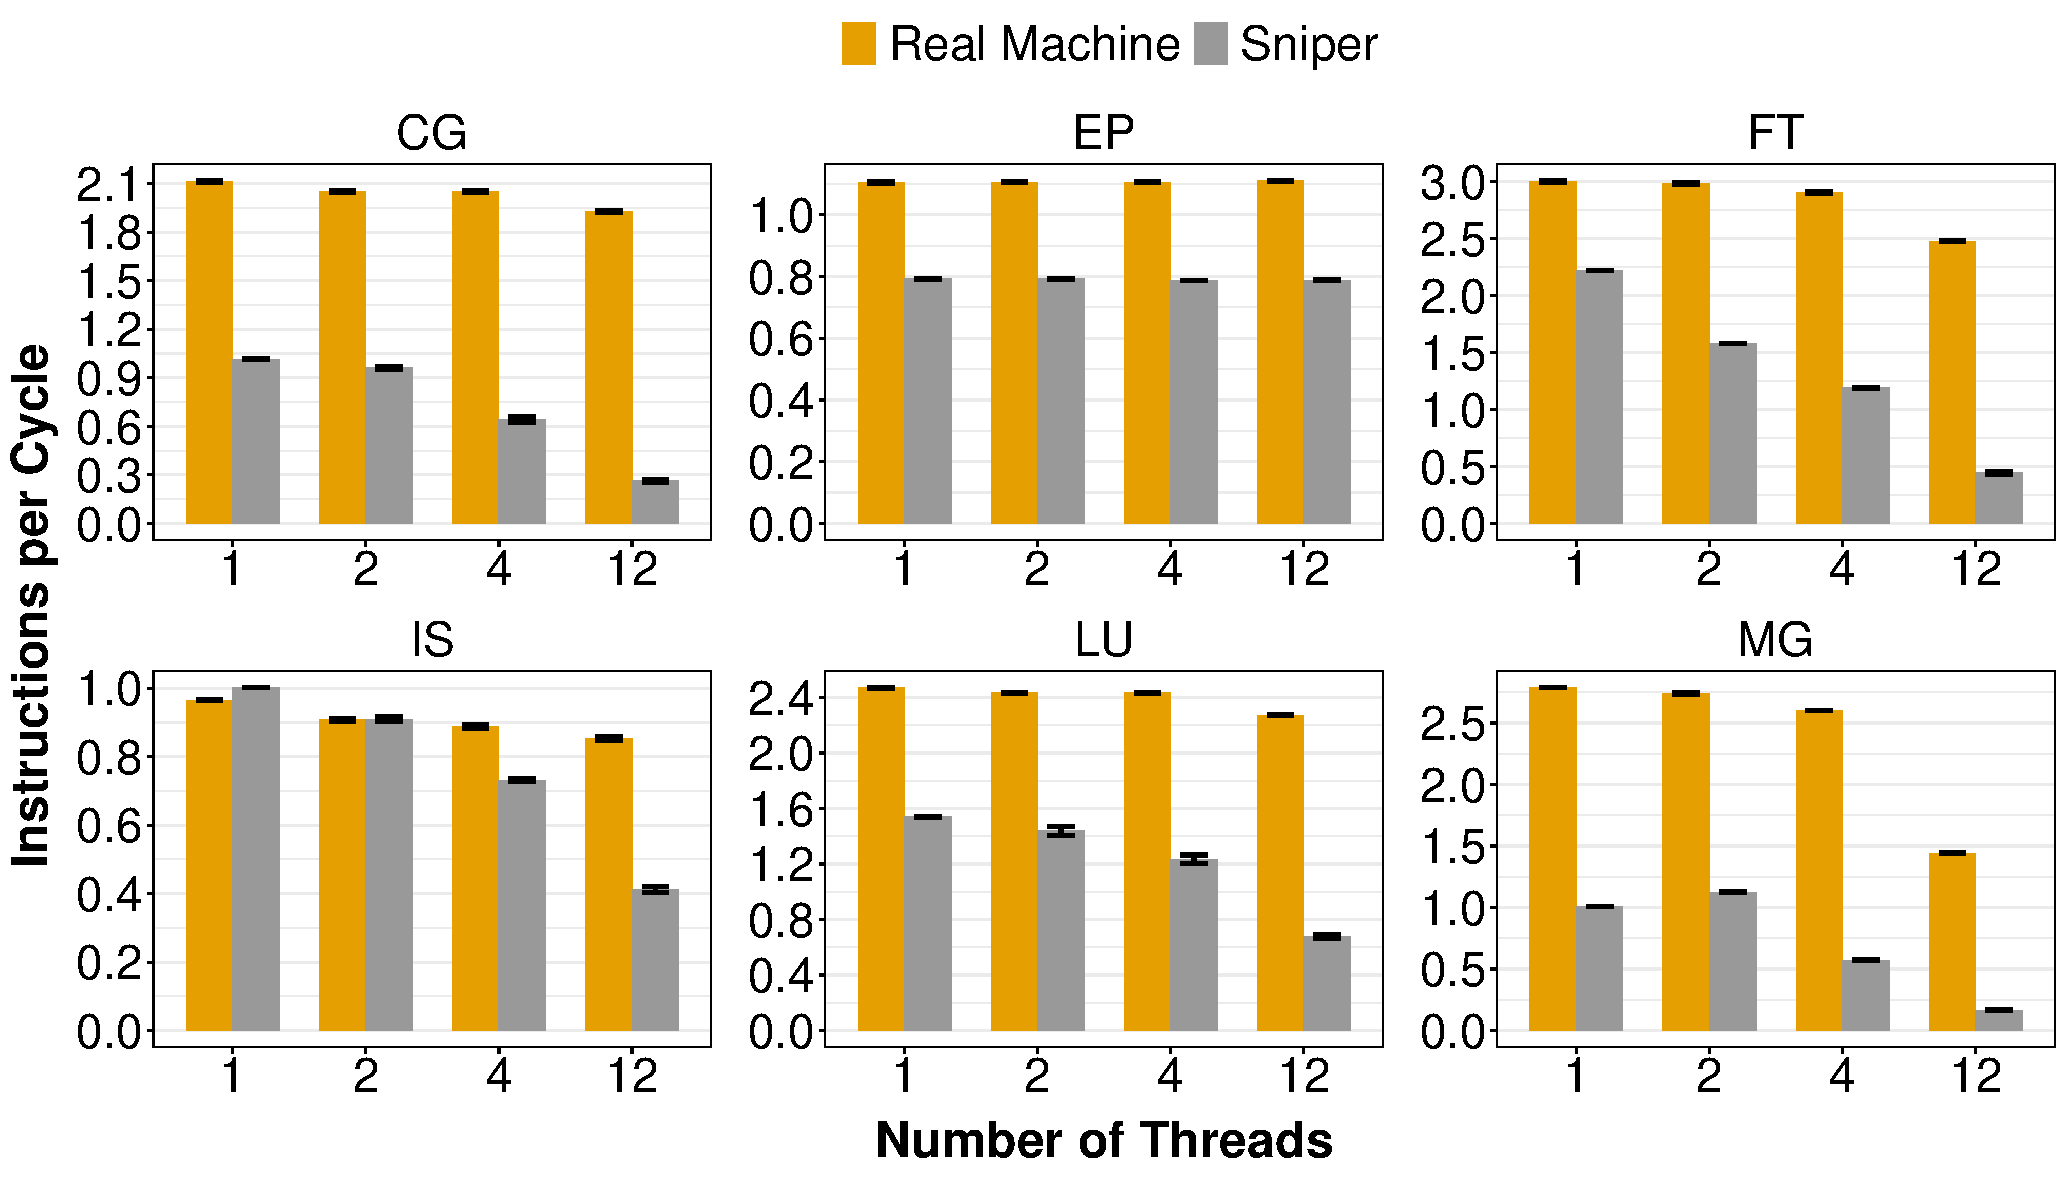
\includegraphics[width=\linewidth]{figures/fig10.pdf}
%     \caption{Performance results of Sniper's L1+L2 prefetchers simulation and real hardware with L1+L2 prefetchers.}
%     \label{fig:sniper_l1l2}
% \end{figure}

As aforementioned, accurately modeling contention is challenging. 
As mentioned in Section~\ref{ref:subs_zsim}, in ZSim's case it is assumed that most concurrent accesses happen to unrelated cache lines when considering small time scales. 
In that way, ZSim was engineered in such a way that requests to the same cache line may be simulated in a different order than the observed in the real execution~\cite{sanchez2013zsim}.
Therefore, the path of the data through the cache hierarchy may change, resulting in simulation inaccuracies.
This may explain the discrepancies of ZSim when simulating CG, as it is straightforward to devise that the concurrent and irregular memory accesses present in CG lead to concurrent accesses in same cache lines.
This same explanation can also be the case for the LU application, though a more detailed memory access analysis of LU is required to attest this argument.

As a general trend, for NPB applications with communication and contention, ZSim tends to underestimate the contention effects, while Sniper tends to overestimate the contention effects as the number of threads in the simulation increases.
For ZSim, this fact can be due to the above-mentioned design assumptions made during its development. 
For Sniper, in its turn, the reason can be more complicated, as it has been reported~\cite{carlson2014aeohmcm} that simulation errors in Sniper's memory model happen when simulating parallel applications with the interval model (see Section~\ref{subsubsec:sniper}). 

%tempo de acesso diferente dependendo da distância que os dados estão na mesh

%It is notable that for the majority of the applications Sniper apresenta uma notável perda de desempenho conforme se aumenta o número de threads, com exceção do EP.
%Uma possível explicação para esse fenômeno é que, conforme aumenta-se a quantidade de threads, a necessidade de comunicação aumenta a utilização do sistema de memória da simulação do Sniper.
%Em seu próprio relatório de validação, é reportado que conforme aumenta-se o número de threads o erro de simulação aumenta devido a erros na modelagem do sistema de memória simulado~\cite{carlson2014aeohmcm}.


%Uma vez que com mais threads é necessário realizar uma maior comunicação, mais acessos ao último nível de memória cache são necessários.
%Desse modo, em metade das aplicações conforme aumenta-se o número de threads observa-se o efeito da contenção de memória no desempenho das aplicações.
%Os resultados observados com o ZSim mostram que o simulador é capaz de representar de alguma forma a contenção que ocorre, porém não com a mesma intensidade que ocorre nas execuções reais.

%Com relação à aplicação LU, a simulação com o ZSim apresenta um comportamento contrário à tendência da execução em uma máquina real.
%Tal comportamento é obscuro.


%Desse modo, uma thread pode acessar dados trazidos por outra thread muito distante na mesh, cujo o tempo de acesso será muito maior do que o tempo de acesso a um dado trazido por uma thread mais próxima.

% -- ZSim não simulou direito CG, LU e MG

%\textcolor{red}{\textbf{DCS:} Questões a serem respondidas:\\2- Por quê o ZSim tem o comportamento de IPC contrário a execução real na app LU (IPC aumenta com mais threads, deveria cair)\\3- Nos dados de simulação novos, temos os equivalentes aos Número de acessos à cache LLC e  Número de acessos à cache L1 de dados, que são os dados mostrados no paper do WSCAD?\\4- De todas as métricas de prefetcher que temos agora, qual seria a mais importante (MPKI-Misses Per Kilo Instructions?)}
%1- Por quê o Sniper cai tanto o IPC em função do número de threads\\




%\vsg{arrumar texto figuras mudaram}
%\textcolor{red}{\textbf{labels fig:sniper\_l1l2 agora sao tambem fig:sniper\_l2 }}
\textbf{In Figure~\ref{fig:sniper_l2}}, we compare the performance, in terms of IPC, of the Sniper's L2 prefetcher with the L2 prefetcher of the real machine, and the Sniper's L1+L2 prefetcher with the real counterpart, respetively.
In all evaluated NPB applications, we can notice discrepancies between the Sniper simulation results and the real machine results, with Sniper mostly underestimating the IPC performance, and overestimating the communication and contention effects with increasing number of threads.
Many reasons can explain this fact. 
First, as mentioned above, Sniper presents errors in its memory model when simulating parallel applications, even without considering prefetcher. 
These errors may be further amplified by adding a memory prefetcher in the simulation. 
Second, Global History Buffer (GHB)~\cite{nesbit2004data} L2 prefetcher implemented in Sniper differs from the Skylake's Stream~\cite{intelmanual} L2 prefetcher. 
In this regard, the GHB prefetcher offered by Sniper may not be suited to simulate Skylake. 
Modeling prefetcher algorithms with the same level of specificity of the real algorithms may be unfeasible, unfortunately, since manufaturers need to conceal key characteristics of their products (including prefetcher algorithms) in order to stay competitive.
\new{Another point worth noting is that, as mentioned in Section~\ref{subsec:exp-setup}, Skylake implements a non-inclusive L3 cache.
This non-inclusive L3 adds new complexity to the memory subsystem simulation since the data's location in this new organization depends upon several aspects~\cite{intelmanual}.}
Similarly to other architecture simulators, Sniper implements an inclusive L3 cache. This difference can also contribute to the discrepancies between the real execution using Skylake and the Sniper simulation.
% Second, the Global History Buffer~\cite{nesbit2004data} implemented in Sniper may not contain specificities that are probably present in the Skylake hardware prefetchers. 
%This second point may remain open, unfortunately, since manufaturers need to conceal key characteristics of their products (including prefetcher algorithms) in order to stay competitive.

%Várias razões explicam esse fato.
%Uma vez que o Sniper já apresenta resultados discrepantes sem a simulação do prefetcher, quando considera-se o comportamento do prefetcher simulado, esses erros podem se tornar ainda maiores.
%Além disso, não há garantias de que o modelo de prefetcher implementado pelo Sniper seja de fato similar ao que é encontrado no hardware da cache L2 da Skylake, uma vez que as implementações são fechadas.
%Outro ponto a se destacar é que o Sniper sempre apresenta valores de IPC menores quando comparado com a execução real.
%Tal comportamento não é observado na simulação do Sniper sem prefetcher, como mostra a Figura~\ref{fig:sims_nopref}.
%Isso tanto pode ser resultado da imprecisão na implementação do prefetcher, como mencionado acima, quando pode ser resultado da dificuldade de se modelar os arquivos de configuração da simulação novamente devido à confidencialidade do hardware real.



%\vsg{Something else that I want to look into is how sniper implements caches inclusiveness, since in skylake the LLC is non-inclusive. With a L3 non-inclusive, what is stored where will depend on the particular access pattern of the executing application, the size of code and data accessed, and the inter-core sharing behavior (the L2 prefetcher also can prefetch data into the L2 or directly into the LLC (https://software.intel.com/en-us/forums/software-tuning-performance-optimization-platform-monitoring/topic/703019)). In sniper they probably only implement an inclusive LLC. How does it affect the results we have?}
%Notes about the sniper memory subsystem implementation: They improved the interval simulation model by improving how the dependent memory accesses are handled (pending hits and dependents of independent long-latency loads).-> When showing the results for the multicore simulation, they mention that "errors goes up with increasing core count, \textbf{mostly because of erros in Sniper's memory hierarchy modeling}. As example they show radix, a benchmark that experiences a large number of TLB misses, and queuing delays caused by the write-back of evicted dirty cache lines push the limits of the level of detail provided in the memory hierarchy."Basically, they're admitting that when the memory subsystem gains relevance in the application performance, the simulation error becomes bigger (all this is mentioned in their TACO paper).

%\fbm{hwat}
%O comportamento do sniper com L1 + L2 na Figura~\ref{fig:sniper_l1l2} fica mais coerente pra todas as apps.
%Ainda assim, há dúvidas sobre o quão corretas são as implementações e também as configurações de prefetcher usadas na simulação.
%Pode ser que o modelo de prefetcher utilizado pra L2 nas simulações seja mais preciso (algo semelhante ao http://www.eecg.toronto.edu/~steffan/carg/readings/ghb.pdf), até pq o outro modelo era um simples.


%Sempre importante lembrar que o prefetcher do Sniper não é validado para x86 \fbm{lies, foi validado pra ARM, ver RW, modifiquei aqui pra "n foi validado em x86"}  (em sua validação o prefetcher foi desabilitado na máquia real).
%Também é importante ressaltar que na arquitetura Skylake a memória cache L3 é não inclusiva, enquanto que a maior parte dos simuladores modela caches L3 inclusivas.
%Um estudo mais detalhado sobre os impactos dessa diferença de modelagem da cache L3 é necessário.

% Please add the following required packages to your document preamble:
% \usepackage{booktabs}
% \usepackage{multirow}

\begin{table}[]\centering
\caption{Total number of prefetches issued by the simulation and by the real hardware.}
\label{table:num_pref}
\begin{tabular}{@{}ccccccccc@{}}
\multicolumn{1}{c|}{\multirow{2}{*}{\textbf{Applications}}} & \multicolumn{4}{c|}{\textbf{Sniper L2}}              & \multicolumn{4}{c}{\textbf{Real L2}}      \\ \cmidrule(l){2-9} 
\multicolumn{1}{c|}{}                                       & 1      & 2      & 4     & \multicolumn{1}{c|}{12}    & 1         & 2        & 4        & 12      \\ \midrule
\multicolumn{1}{c|}{\textbf{CG}}                            & 18.6   & 8.9    & 4.4   & \multicolumn{1}{c|}{1.6}   & 155.0     & 121.4    & 47.8     & 16.9    \\
\multicolumn{1}{c|}{\textbf{EP}}                            & 0.0    & 0.0    & 0.0   & \multicolumn{1}{c|}{65.6}  & 81.3      & 41.7     & 20.3     & 6.8     \\
\multicolumn{1}{c|}{\textbf{FT}}                            & 67.6   & 33.7   & 17.1  & \multicolumn{1}{c|}{5.9}   & 94.4      & 48.8     & 25.9     & 10.1    \\
\multicolumn{1}{c|}{\textbf{IS}}                            & 99.5   & 35.2   & 16.8  & \multicolumn{1}{c|}{5.8}   & 21.1      & 16.9     & 8.8      & 2.3     \\
\multicolumn{1}{c|}{\textbf{LU}}                            & 845.8  & 434.3  & 225.0 & \multicolumn{1}{c|}{82.6}  & 4251.1    & 2069.3   & 449.3    & 104.8   \\
\multicolumn{1}{c|}{\textbf{MG}}                            & 455.3  & 306.9  & 189.5 & \multicolumn{1}{c|}{64.7}  & 318.0     & 158.5    & 72.1     & 24.3    \\
                                                            &        &        &       &                            &           &          &          &         \\ \midrule
\multicolumn{1}{c|}{\multirow{2}{*}{\textbf{Applications}}} & \multicolumn{4}{c|}{\textbf{Sniper L1 + L2}}         & \multicolumn{4}{c}{\textbf{Real L1 + L2}} \\ \cmidrule(l){2-9} 
\multicolumn{1}{c|}{}                                       & 1      & 2      & 4     & \multicolumn{1}{c|}{12}    & 1         & 2        & 4        & 12      \\ \cmidrule(l){2-9} 
\multicolumn{1}{c|}{\textbf{CG}}                            & 366.2  & 182.6  & 91.4  & \multicolumn{1}{c|}{30.6}  & 298.5     & 195.0    & 84.4     & 28.8    \\
\multicolumn{1}{c|}{\textbf{EP}}                            & 133.1  & 66.5   & 33.3  & \multicolumn{1}{c|}{11.1}  & 113.4     & 57.6     & 28.6     & 9.6     \\
\multicolumn{1}{c|}{\textbf{FT}}                            & 489.9  & 252.3  & 126.9 & \multicolumn{1}{c|}{42.4}  & 473.4     & 238.6    & 120.5    & 41.5    \\
\multicolumn{1}{c|}{\textbf{IS}}                            & 34.5   & 17.8   & 8.9   & \multicolumn{1}{c|}{3.0}   & 37.3      & 24.7     & 14.3     & 4.2     \\
\multicolumn{1}{c|}{\textbf{LU}}                            & 3359.4 & 1698.9 & 862.0 & \multicolumn{1}{c|}{286.5} & 6430.9    & 3173.0   & 1017.6   & 292.2   \\
\multicolumn{1}{c|}{\textbf{MG}}                            & 452.0  & 202.7  & 112.8 & \multicolumn{1}{c|}{42.0}  & 543.7     & 271.2    & 124.0    & 40.8   
\end{tabular}
\end{table}


\begin{figure}[b]
    \centering
    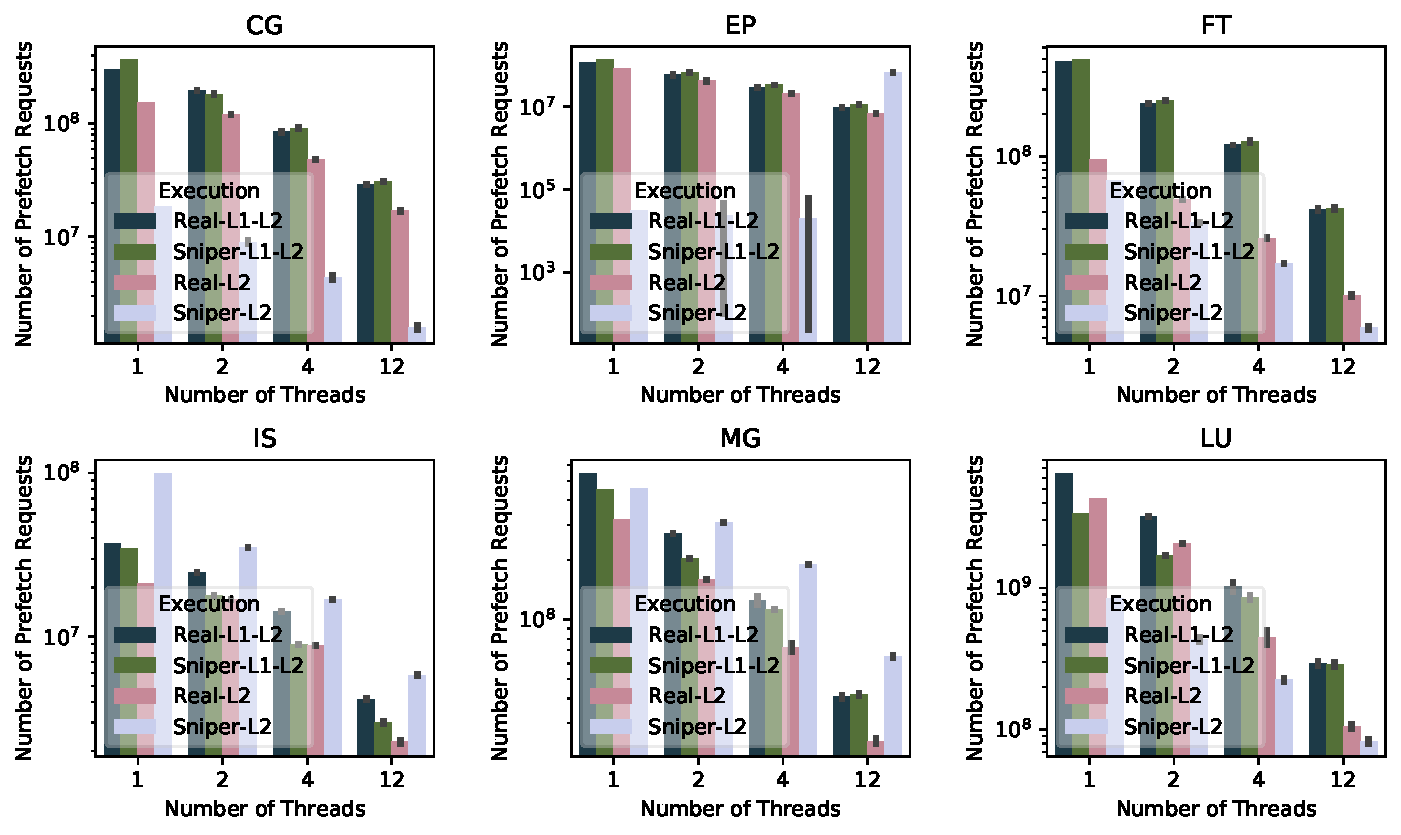
\includegraphics[width=.8\linewidth]{figures/sniper_l2-rqsts-all-pf.pdf}
    \caption{Total number of prefetches issued by the simulation and by the real hardware (log scale on $y$ axis).}
    \label{fig:sniper_l2-rqsts-all-pf}
\end{figure}


In Figure~\ref{fig:sniper_l2-rqsts-all-pf} we present the total number of prefetch requests performed by the Sniper's L1+L2 prefetcher, the Sniper's L2 prefetcher, and their real counterparts. The number of prefetch requests for the L1+L2 prefetcher counts the prefetches on both L1 and L2 caches.
As expected at this point, Sniper's L2 prefetcher model was not capable to accurately simulate the Skylake's L2 prefetcher on the number of prefetch requests as well, presenting large discrepancies (notice the log scale on the $y$ axis of Figure~\ref{fig:sniper_l2-rqsts-all-pf}).
On the other hand, Sniper's L1+L2 prefetcher presented a total number of prefetch requests closer to the real execution. 
However, the similar number of prefetch requests of the Sniper's L1+L2 prefetchers does not translate in similar estimations of the applications performance, as shown in Figure~\ref{fig:sniper_l2}.
This may be due to the fact that the prefetches performed by Sniper are different in terms of usefullness. 
To attest this argument, in Figure~\ref{fig:sniper_useless_pf_ratio} we show the mean percentage of prefetches that were not useful during the executions in the real machine and in the Sniper simulation.
We can notice that the only application that sniper managed to accurately simulate the usefullness of the prefetches is the FT application.
%\textcolor{blue}{\textbf{DCS:Alguém dá uma aprimorada no parágrafo abaixo plz}}
When simulating the other applications with Sniper, Sniper considered the majority of prefetch requests as useless, with useless prefetches close to 100\% in some cases. 
This may indicate that Sniper's memory simulation module is having issues on simulating how the prefetched data is interacting with cache hierarchy. 
The non-inclusive L3 cache may also be a cause of this issue, since again Sniper considers an inclusive L3 cache.

%In this regard, it is important to remember that Sniper's L1+L2 prefetcher is an L1 prefethcer algorithm, executing in conjunction with an L2 prefetcher algorithm (which is the same algorithm used in the Sniper's ``L2 prefetcher'') (see Section~\ref{subsec:exp-setup}). 
%At this light, we can argue that the Sniper's L1 prefetcher algorithm (as opposed to the L2 prefetcher algorithm) is the one that is effectively contributing to a more accurate simulation, at least in the number of prefetch requests

%Na Figure~\ref{fig:sniper_l2-rqsts-all-pf} é possível observar a quantidade de requisições de prefetch que são issued em cada um dos experimentos.
%A primeira informação nítida é a discrepância observada nos resultados que consideram apenas o prefetcher da cache L2 ativado.
%Como já citado anteriormente na Section~\ref{subs:simulation}, o prefetcher oferecido pelo Sniper e utilizado como algoritmo para a cache L2 é o Global History Buffer, diferente do encontrado no hardware da máquina real que é um streamer, o que facilmente explica as discrepâncias observadas.

%\vsg{melhorar}
%Quando se considera ambos os prefetches das caches L1 e L2, é possível ver que a quantidade de prefetchers sendo realizada segue as tendências das execuções reais, o que indica que o comportamento dos prefetchers modelados pelo sniper pode estar correto.
%No entanto, pra termos certeza, a gente precisa analisar a eficácia dos prefetches realizados (timeliness, useless, ...), pois o número pode ser parecido, porém podem estar sendo feitos prefetches por linhas de cache incorretas ou não úteis...
%Além disso, mesmo que os prefetches estejam corretos, a diferença no IPC continua podendo ser explicada pela dificuldade de modelar-se os efeitos da contenção de recursos que são compartilhados no processador.
%Counters the usabilidade têm significados diferentes no sniper e na máquina real.






\begin{figure}
    \centering
    %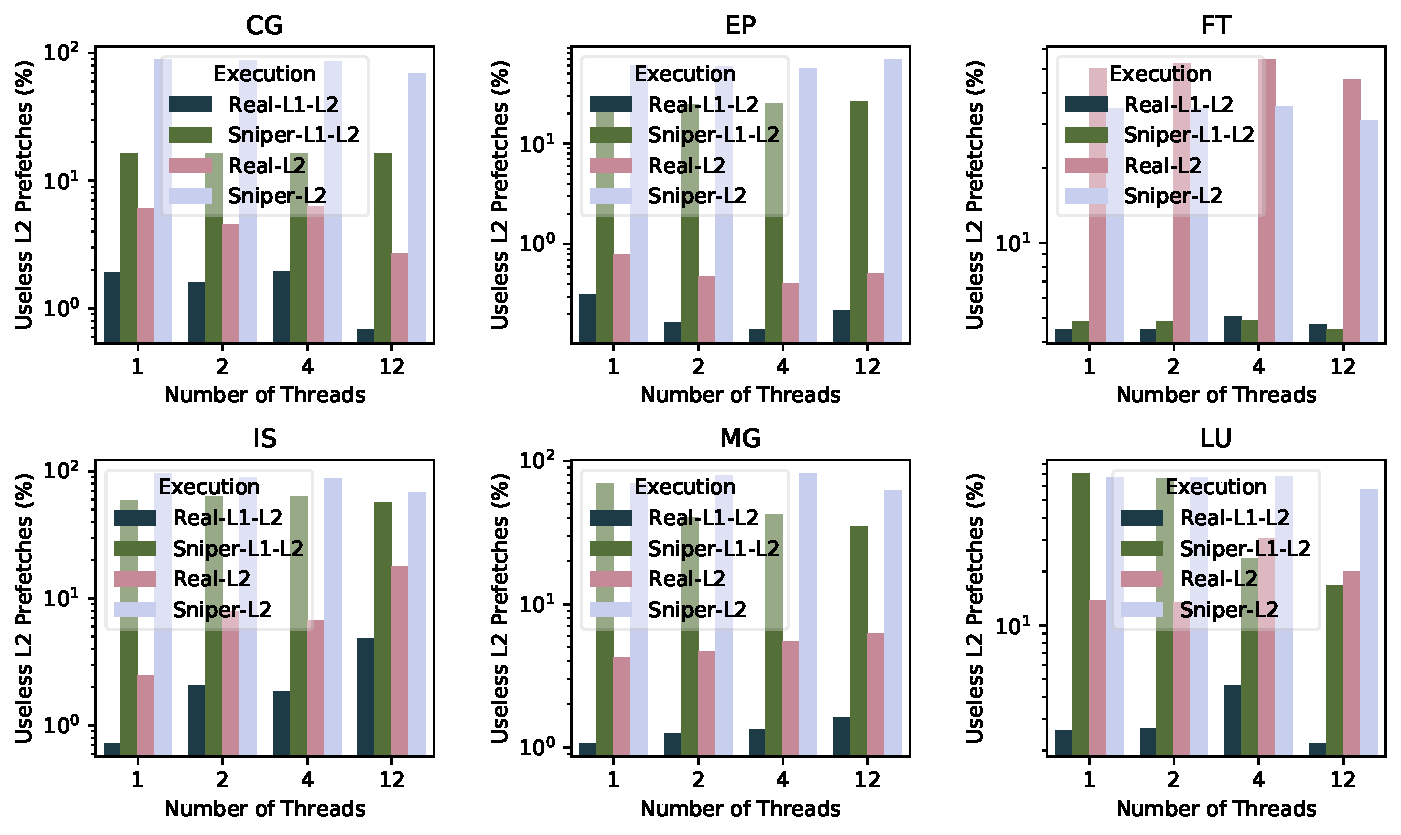
\includegraphics[width=.8\linewidth]{figures/sniper_useless_pf_ratio.pdf}
    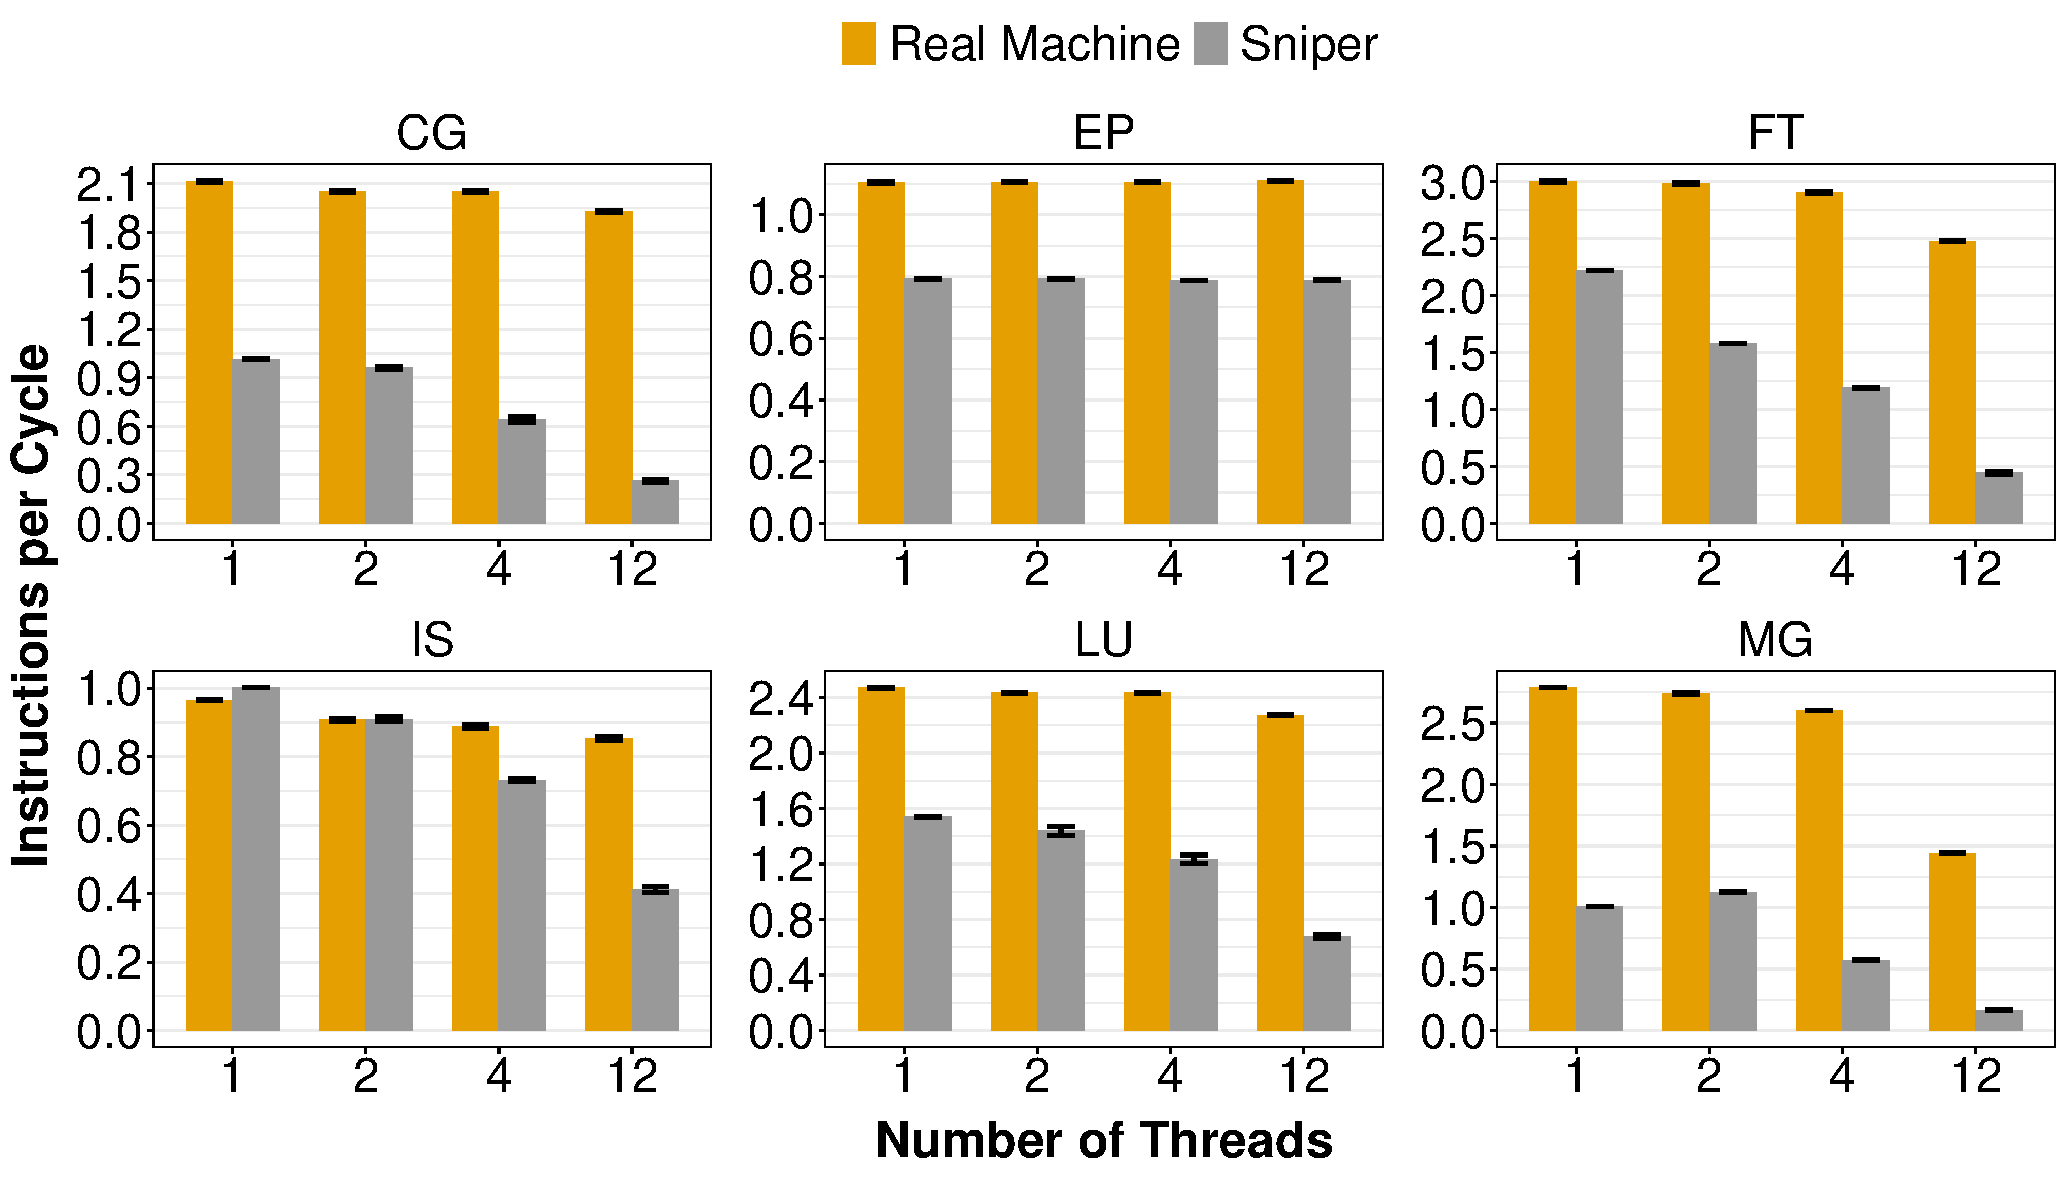
\includegraphics[width=\linewidth]{figures/fig10.pdf}
    \caption{Useless prefeteches performed by the simulation and by the real hardware, in ratio of the total number of prefetches.}
    \label{fig:sniper_useless_pf_ratio}
\end{figure}






%\begin{figure}
%    \centering
%    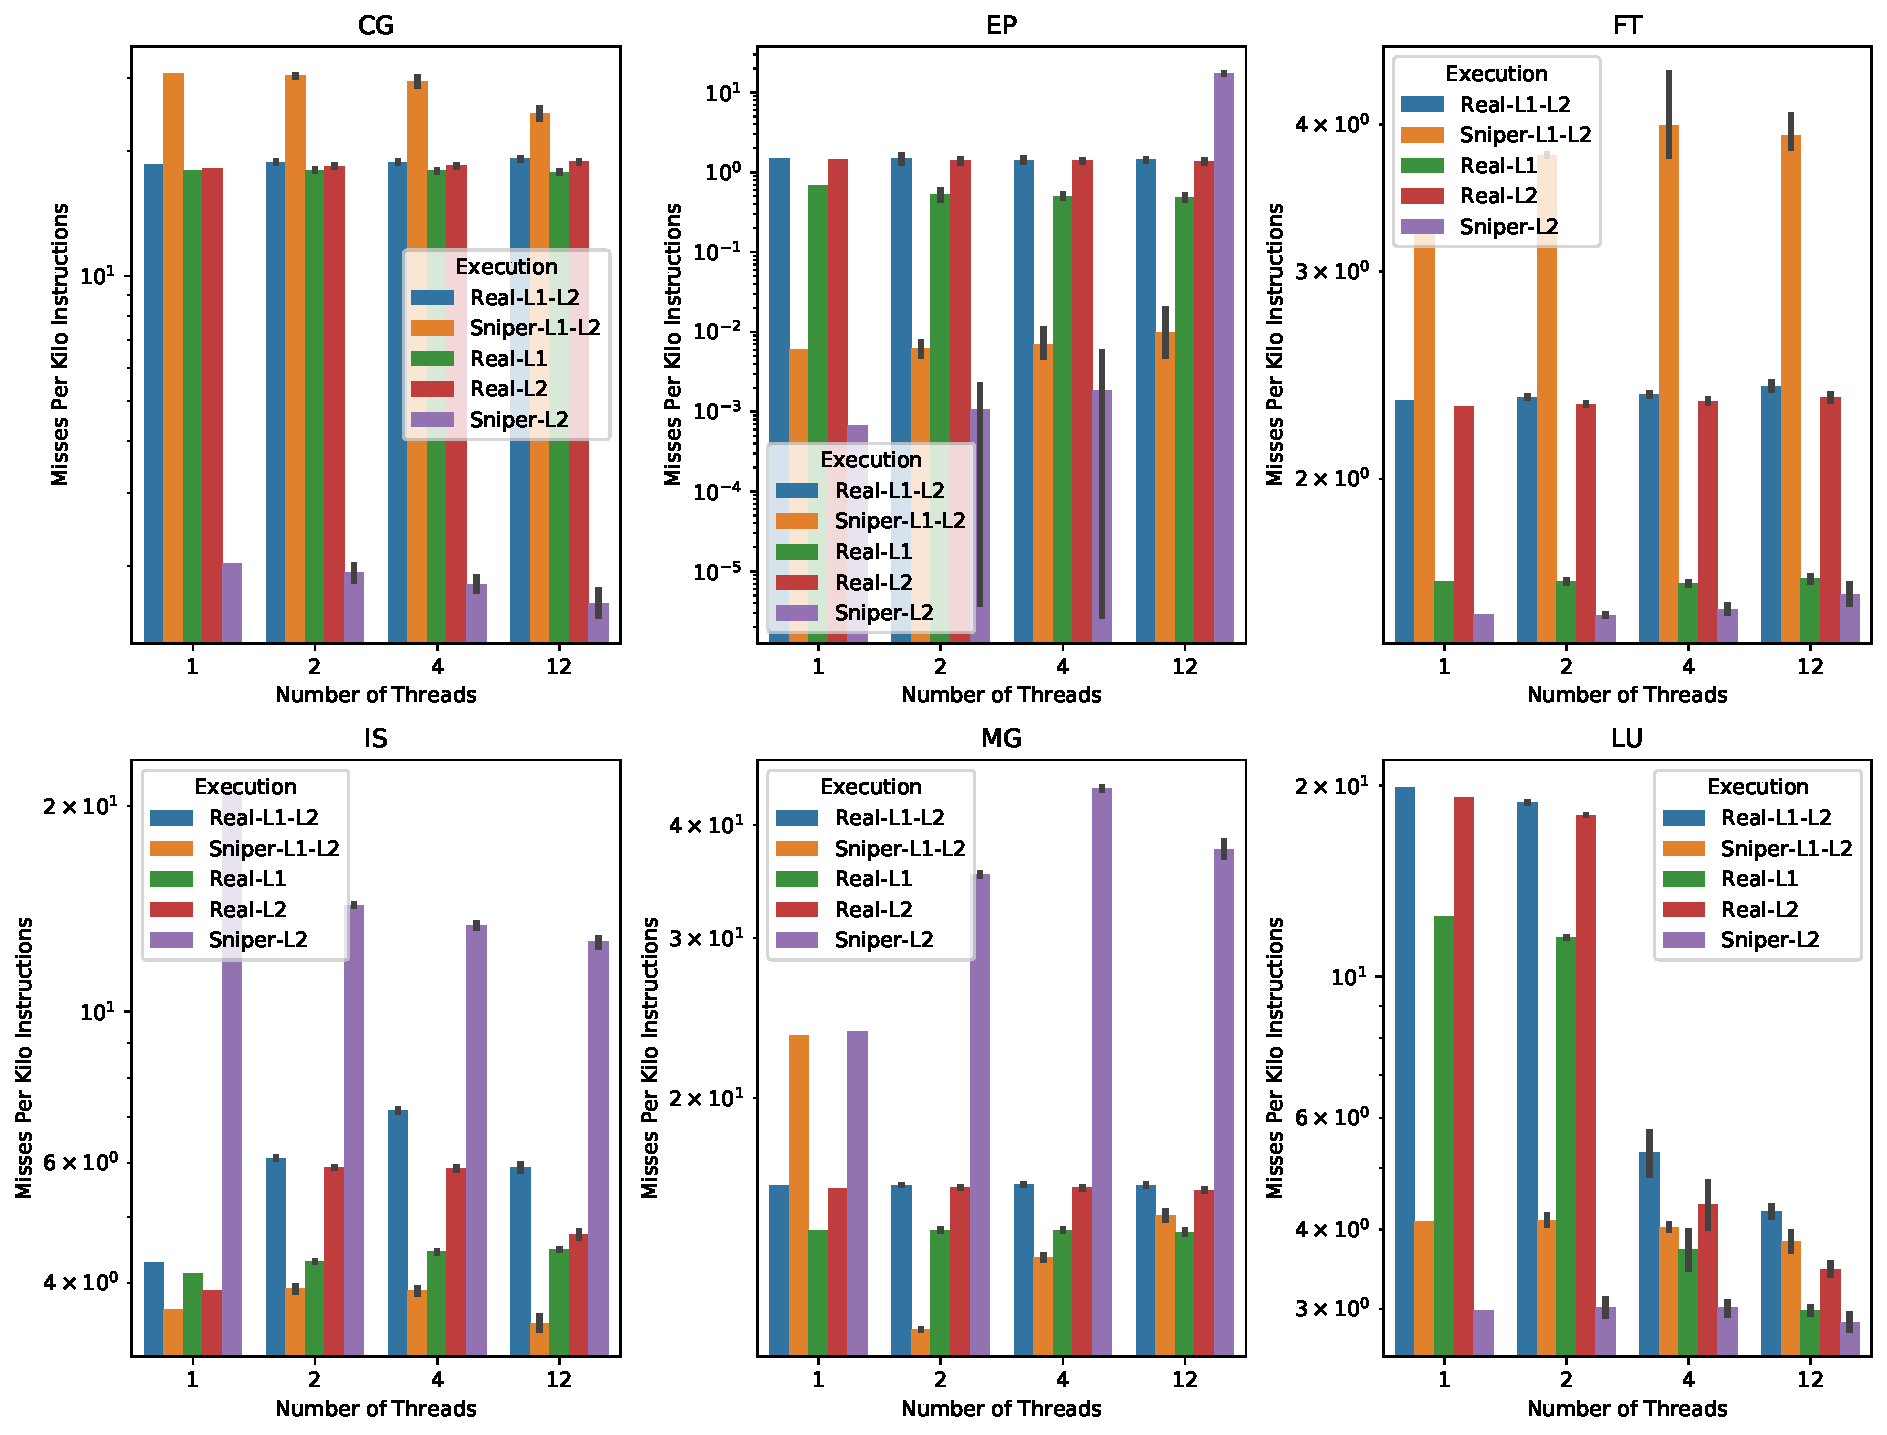
\includegraphics[width=.8\linewidth]{figures/sniper_mpki.pdf}
%    \caption{Sniper Misses Per Kilo Instructions}
%    \label{fig:sniper_mpki}
%\end{figure}



\section{Discussion and Guidelines}\label{sec:insights}

An important aspect highlighted throughout the entire work is the difficulty of working with the memory subsystem, with the prefetcher and its algorithms being a special case.
The obscurity and confidentiality around the real implementation makes accurate models and algorithms impossible to be reproduced in simulators; moreover, for the same reasons above, simulator users have difficulties even in finding the proper parameters for the prefetcher models.

%Referente às observações encontradas nos experimentos, encontramos diversas características nos prefetchers estudados que são interessantes e que podem orientar a trabalhos futuros.
Regarding the observations we made in the experiments, we found several interesting characteristics in the studied prefetchers that may direct future works.
%Primeiramente, notou-se diversas vantagens do prefetcher da cache L2 se comparado ao prefetcher da cache L1.
%First, the L2 data prefetcher has shown to be much more relevant than the L1 data prefetcher.
%Na Section~\ref{subsubsec:real_ipc} foi discutido como o prefetcher da cache L1 ocupa uma porção significativa do hardware e como sua implementação é menos clara que os demais prefetchers.
We have discussed how the L1 data prefetcher snooping the L1 cache requests can create contention by occupying the limited line fill buffers in the L1 cache.
\vsg{ver essa afirmacao aqui tbm} \textcolor{red}{\textbf{eu removeria, até pq a gente fala de line fill buffers apenas aqui no paper}}
Moreover, the obscurity of the L1 prefetcher implementation makes architecture studies that consider the L1 prefetcher harder to interpret.
%Com isso, estudos sobre arquitetura de computadores que consideram o prefetcher da L1 podem ser mais difíceis de ser interpretados
%Além disso, analisar o desempenho de aplicações se torna mais complicado devido à falta de clareza e conhecimento pleno que se possui sobre os prefetcher e suas implementações.
Analyzing applications' performance, therefore, becomes harder due to the lack of control over the prefetchers and their implementations.

%Moreover, na mesma seção supracitada discute-se que a utilização de ambos os prefetchers L1+L2 não necessariamente garante ganhos significativos de desempenho, o que de certa forma contraria o que é esperado.
We argue that the use of both prefetchers (L1+L2) does not necessarily warrant significant performance gains, which is not intuitive.
%Quando utiliza-se apenas o prefetcher da L2, obtem-se ganhos de desempenho similares a ambos os prefetchers juntos, porém com a vantagem de muito mais transparência.
When considering the L2 prefetcher, we obtained performance gains similar to when using both prefetchers, with the advantages of having more control over the experiments and the noise in the memory subsystem, faster simulation time, and thus less energy consumption due to the smaller number of \new{prefetch} requests being performed. 
%Isto é compreensível uma vez que atualmente as tecnologias de memória cache permitem pouca diferença no tempo de acesso das caches L1 e L2.
This is comprehensible, as the current cache memory technologies allow a small difference in latency between the L1 and L2 caches, and \new{avoiding accesses to} the L3 cache becomes more critical in terms of latency.
%No entanto, a latência de acessos que são direcionados à cache L3 é consideravelmente maior (\textbf{XX s numeros aqui}), tanto por distinções tecnológicas quanto por questões de topologia da mesh de interconexão -- quanto mais núcleos estão sendo utilizados na execução, mais complexa é a rede de interconexão.
\new{The access latency to the off-chip L3 cache memory is considerably higher than the access latency of the L2 cache (on average 7x, due to the mesh topology necessary to fully utilize the cache, as it is distributed in L3 off-core banks).}
%Portanto, aconselhamos o uso do prefetcher da L2 ao invés de ambos os prefetchers (L1+L2, configuração padrão do hardware), pois é mais importante evitar acessos à L3 do que à L2, e devido à maior transparência do prefetcher da L2.
Therefore, we advise using the L2 prefetcher as a standalone instead of both prefetchers (which is the default setting).
The L2 prefetcher observes the more relevant access patterns, as it prefetches data that would always require an access to the L3, thus hiding the large L3 latency.


With the increase in application parallelism, the execution time naturally becomes smaller. 
However, we see that the performance per core decreases as we increase the level of parallelism, showing the impact of memory accesses and communication over the application's performance.
As the amount of communication increases, the contention for the shared resources (interconnection network and LLC banks) increases as well.
Thereby, the request buffers of the caches and main memory become full, and the prefetcher cannot sufficiently mitigate the memory latency, resulting in small IPC values.
Thus, analyzing the communication pattern of applications is an important task to improve their performance, as applications which exert heavy memory pressure or communicate often can diminish the usefulness of a prefetcher.

\subsection{Considerations About the Prefetcher's Usefulness Degradation}
\label{subsec:pref_usefulness_thoughts}
In recent years, Intel implemented forms of reducing the prefetcher aggressiveness due to multiple reports such as Dell's \vsg{a gente so joga essa info aqui do nada?}, in order to avoid performance degradation.
Our real execution results show that even with high parallelism, Intel's strategy works, as the prefetcher never loses performance compared to an execution without prefetchers.
However, it would be interesting to test this assumption with simultaneous multithreading.

Nevertheless, our research shows that computer architecture researchers should always implement a prefetcher aggressiveness attenuator in the simulator model, and test their new implementations on highly parallel applications which exert memory pressure and inter-core interference~\cite{ebrahimi2009coordinated}, so that the possible negative impacts of their design can be properly evaluated.
%We hope that the observations present in this paper guide future memory prefetcher simulation research, and notably Sniper's development, by sheding light on the prefetch usefullness issue (see Figure~\ref{fig:sniper_useless_pf_ratio}) observed in our experiments.
%Unfortunately, this is not the case for several works in the last two years.

\subsection{Generalization to Other Applications}
\label{subsec:other_apps}
%\vsg{repete demais a palavra embarrassingly aqui, da pra usar simplesmente aplicacoes trivialmente paralelizaveis, mas tem que achar um bom termo em ingles kk}
We generalized a set of application characteristics during our experimental investigation, so that the results observed during this work -- specially the degradation of the prefetcher's usefulness as the level of parallelism increases -- can also be applicable for other types of applications. 
One of the main characteristics is about if a parallel application is embarassingly parallel -- which, for text clarity, we abbreviate to \textit{EmbPar} -- or not. 
Our observations can be extended for (i) any non-EmbPar application, and for (ii) EmbPar applications with in-place memory operations. Many parallel applications are non-EmbPar since EmbPar preventing operations such as locking and synchronization are often required in parallel algorithms (e.g., parallel Map Reduce or Stochastic Gradient Descent). EmbPar applications with in-place memory operations are less common, such as the pseudo-random number generation performed by the EP application of NPB. Our observation's exceptions are EmbPar applications that operate over vectors/matrices, such as parallel vector sum or matrix multiplication. These applications do not suffer from contention caused by synchronization or locking and may benefit from prefetchers since the number of memory accesses of these applications is significant.

%High performance computing users should be aware of this.
Some practitioners have experienced this degradation of the prefetcher's usefulness in other applications, such as the experiences reported by Dell~\cite{SAPguide}, which claim 8\% increased performance for the SAP NetWeaver Portal application when disabling the hardware prefetchers.
%Highly parallel applications may benefit from turning off the prefetcher, as suggested by Dell~\cite{SAPguide}, which claims 8\% increased performance for the SAP NetWeaver Portal application when disabling the hardware prefetchers.

\subsection{Good Practices and Guidelines}
\label{subsec:practices_n_experiences}
In this section, we present a summary of the main scientific and technical findings that we experienced during this work's development. These findings are framed into a list of good practices and guidelines that we suggest for future research and development on memory prefetcher with parallel applications, with and without simulation.

\begin{itemize}
    \item One shall pay attention on how the profiling tool collects performance data. Some profiling tools (such as Perf~\cite{de2010new}) collect performance data in a system-wide manner. In this context, system processes may affect the profiling results. However, when evaluating the performance of applications individually, we are concerned with performance data application-wide. Such data can be collected, for instance, using PAPI~\cite{terpstra2010papi};
    
    \item One shall be careful if a certain architecture research (notably prefetcher research) relies on an evaluation/validation performed by architecture simulators. In our experience, architecture simulators did not accurately represent real architectures, specifically when we consider memory prefetcher and parallel applications. Improving simulators' accuracy is a concerning and essential matter for the future of architecture algorithms research;
    
    \item Research on prefetcher algorithms for the L2 cache seems more promising to yield significant performance improvements -- as opposed to prefetcher algorithms for the L1 cache -- since, in our experience, accessing the L3 cache was a larger detriment to performance, as opposed to accessing the L2 cache;
    
    \item For highly parallel applications (in the order of dozens of threads on a single machine, see Section~\ref{subsec:other_apps}), memory prefetchers may not be critical for the application's performance since, in our experience, the prefetchers' performance seems to be bound to the performance degradation caused by the parallel contention.
\end{itemize}




\section{Conclusion and Future Work}\label{sec:conclusion}
%Ao longo do desenvolvimento deste trabalho, diversos pontos foram aprendidos, tanto no que diz respeito a aspectos metodológicos, quanto no que se refere ao comportamento dos modelos de prefetcher estudados e sua utilização.
Memory prefetcher algorithms have been widely used in processors to mitigate the performance gap between the processors and the memory subsystem. Analyzing and developing new prefetcher algorithms is a notoriously challenging task, especially due to the complexities and obscurities behind computer architecture development.

Memory prefetcher research is mainly possible thanks to architecture simulators that attempt to model the highly complex (and sometimes obscure) interactions present in the hardware. When we account for parallel, High-Performance Computing (HPC) applications, understanding the prefetcher's contribution to performance, on both the real hardware and in the simulations, becomes an important matter. 

In this work we performed an experimental investigation of the prefetcher's role in the performance of parallel, High Performance Computing (HPC) applications. Our investigation included a pioneer study on the prefetcher's performance in a simulated environment, taking the Sniper simulator as an example. Several insights were obtained regarding methodological aspects, the behavior of the studied prefetcher models, and how researchers and end users should handle prefetchers, in a both real and simulated scenario. 
%\textcolor{red}{\textbf{dcs: recortei/colei o texto que tava aqui na discussão, pq era um texto de discussão de fato hehe}}

Among these insights, one can highlight: (i) prefetching from the L3 to L2 cache presents a more substantial contribution to performance, (ii) memory contention becomes a larger constraint in the performance as the level of parallelism increases, limiting the prefetcher's contribution, (iii) Skylake's parallel memory contention is poorly simulated by ZSim and Sniper, and (iv) Skylake's non-inclusive L3 cache hinders the accurate simulation of NPB with the Sniper's prefetchers.




\vsg{escrever de forma mais completa, so botei ideias, e tbm ver se eu escrevi certo sobre edp pq eu nao tenho tanta familiaridade}
As future work, we intend to analyze the impact on energy consumption of each prefetcher combination on Skylake.
Since some prefetcher combinations are performing unnecessary costly DRAM accesses, it is relevant to evaluate how these inaccurate prefetch requests impact energy consumption.
Metrics as energy-delay product (EDP)~\cite{gonzalez1996edp} may help us to understand which prefetcher configurations are more suitable considering both energy efficiency and execution time.


%How to measure contention in the LLC? This is required to validate the hypothesis raized in the results section.

%Analisar o quão úteis tão sendo esses prefetchers realizados pelo sniper (timeliness, ...)

%mais benchmarks, apps reais
\section*{Acknowledgements}
This work has been partially supported by Petrobras (2016/00133-9, 2018/00263-5) and Green Cloud project (2016/2551-0000 488-9), from FAPERGS and CNPq Brazil, program PRONEX 12/2014. This study was financed in part by the Coordenação de Aperfeiçoamento de Pessoal de Nível Superior - Brasil (CAPES) - Finance Code 001. Experiments presented in this paper were carried out using the PCAD infrastructure, \url{http://gppd-hpc.inf.ufrgs.br}, at INF/UFRGS.

\bibliography{2020-ccpe-valeria}

\end{document}